\ifx\wholebook\relax \else
% ------------------------

\documentclass[UTF8]{article}
%------------------- Other types of document example ------------------------
%
%\documentclass[twocolumn]{IEEEtran-new}
%\documentclass[12pt,twoside,draft]{IEEEtran}
%\documentstyle[9pt,twocolumn,technote,twoside]{IEEEtran}
%
%-----------------------------------------------------------------------------
%
% loading packages
%

\RequirePackage{ifpdf}
\RequirePackage{ifxetex}

%
%
\ifpdf
  \RequirePackage[pdftex,%
       bookmarksnumbered,%
              colorlinks,%
          linkcolor=blue,%
              hyperindex,%
        plainpages=false,%
       pdfstartview=FitH]{hyperref}
\else\ifxetex
  \RequirePackage[bookmarksnumbered,%
               colorlinks,%
           linkcolor=blue,%
               hyperindex,%
         plainpages=false,%
        pdfstartview=FitH]{hyperref}
\else
  \RequirePackage[dvipdfm,%
        bookmarksnumbered,%
               colorlinks,%
           linkcolor=blue,%
               hyperindex,%
         plainpages=false,%
        pdfstartview=FitH]{hyperref}
\fi\fi
%\usepackage{hyperref}

% other packages
%--------------------------------------------------------------------------
\usepackage{graphicx, color}
\usepackage{subfig}
\usepackage{tikz}
\usetikzlibrary{matrix,positioning}

\usepackage{amsmath, amsthm, amssymb} % for math
\usepackage{exercise} % for exercise
\usepackage{import} % for nested input

%
% for programming
%
\usepackage{verbatim}
\usepackage{listings}
%\usepackage{algorithmic} %old version; we can use algorithmicx instead
\usepackage{algorithm}
\usepackage[noend]{algpseudocode} %for pseudo code, include algorithmicsx automatically
\usepackage{appendix}
\usepackage{makeidx} % for index support
\usepackage{titlesec}

\usepackage[cm-default]{fontspec}
\usepackage{xunicode}

% detect and select Chinese font
% ------------------------------
% the following cmd can list all availabe Chinese fonts in host.
% fc-list :lang=zh
\def\myfont{STHeiti}  % Under Mac OS X
\def\linuxfallback{WenQuanYi Micro Hei} % Under Linux
\def\winfallback{SimSun} % Under Windows
\suppressfontnotfounderror1 % Avoid setting exit code (error level) to break make process
\count255=\interactionmode
\batchmode
\font\foo="\myfont"\space at 10pt
\ifx\foo\nullfont
  \font\foo = "\linuxfallback"\space at 10pt
  \ifx\foo\nullfont
    \font\foo = "\winfallback"\space at 10pt
    \ifx\foo\nullfont
      \errorstopmode
      \errmessage{no suitable Chinese font found}
    \else
      \let\myfont=\winfallback % Windows
    \fi
  \else
    \let\myfont=\linuxfallback % Linux
  \fi
\fi
\interactionmode=\count255
\setmainfont[Mapping=tex-text]{\myfont}

\XeTeXlinebreaklocale "zh"  % to solve the line breaking issue
\XeTeXlinebreakskip = 0pt plus 1pt minus 0.1pt

\titleformat{\paragraph}
{\normalfont\normalsize\bfseries}{\theparagraph}{1em}{}
\titlespacing*{\paragraph}
{0pt}{3.25ex plus 1ex minus .2ex}{1.5ex plus .2ex}

\lstdefinelanguage{Smalltalk}{
  morekeywords={self,super,true,false,nil,thisContext}, % This is overkill
  morestring=[d]',
  morecomment=[s]{"}{"},
  alsoletter={\#:},
  escapechar={!},
  literate=
    {BANG}{!}1
    {UNDERSCORE}{\_}1
    {\\st}{Smalltalk}9 % convenience -- in case \st occurs in code
    % {'}{{\textquotesingle}}1 % replaced by upquote=true in \lstset
    {_}{{$\leftarrow$}}1
    {>>>}{{\sep}}1
    {^}{{$\uparrow$}}1
    {~}{{$\sim$}}1
    {-}{{\sf -\hspace{-0.13em}-}}1  % the goal is to make - the same width as +
    %{+}{\raisebox{0.08ex}{+}}1		% and to raise + off the baseline to match -
    {-->}{{\quad$\longrightarrow$\quad}}3
	, % Don't forget the comma at the end!
  tabsize=2
}[keywords,comments,strings]

% for better Haskell code outlook
\lstdefinelanguage{Haskell}{
  basicstyle=\small\ttfamily,
  flexiblecolumns=false,
  basewidth={0.5em,0.45em},
  literate={+}{{$+$}}1 {/}{{$/$}}1 {*}{{$*$}}1 {=}{{$=$}}1
           {>}{{$>$}}1 {<}{{$<$}}1 {\\}{{$\lambda$}}1
           {\\\\}{{\char`\\\char`\\}}1
           {->}{{$\rightarrow$}}2 {>=}{{$\geq$}}2 {<-}{{$\leftarrow$}}2
           {<=}{{$\leq$}}2 {=>}{{$\Rightarrow$}}2
           {\ .}{{$\circ$}}2 {\ .\ }{{$\circ$}}2
           {>>}{{>>}}2 {>>=}{{>>=}}2
           {|}{{$\mid$}}1
}[keywords,comments,strings]

\lstloadlanguages{C, C++, Lisp, Haskell, Python, Smalltalk}

\lstset{
  showstringspaces = false
}

% ======================================================================

\def\BibTeX{{\rm B\kern-.05em{\sc i\kern-.025em b}\kern-.08em
    T\kern-.1667em\lower.7ex\hbox{E}\kern-.125emX}}

%
% mathematics
%
\newcommand{\be}{\begin{equation}}
\newcommand{\ee}{\end{equation}}
\newcommand{\bmat}[1]{\left( \begin{array}{#1} }
\newcommand{\emat}{\end{array} \right) }
\newcommand{\VEC}[1]{\mbox{\boldmath $#1$}}

% numbered equation array
\newcommand{\bea}{\begin{eqnarray}}
\newcommand{\eea}{\end{eqnarray}}

% equation array not numbered
\newcommand{\bean}{\begin{eqnarray*}}
\newcommand{\eean}{\end{eqnarray*}}

\newtheorem{theorem}{Theorem}[section]
\newtheorem{lemma}[theorem]{Lemma}
\newtheorem{proposition}[theorem]{Proposition}
\newtheorem{corollary}[theorem]{Corollary}


\setcounter{page}{1}
\setcounter{secnumdepth}{4}

\begin{document}

%--------------------------

% ================================================================
%                 COVER PAGE
% ================================================================

\title{搜索}

\author{刘新宇
\thanks{{\bfseries 刘新宇 } \newline
  Email: liuxinyu95@gmail.com \newline}
  }

\maketitle
\fi

\markboth{搜索}{初等算法}

\ifx\wholebook\relax
\chapter{搜索}
\numberwithin{Exercise}{chapter}
\fi

\def\includetikz{}

% ================================================================
%                 Introduction
% ================================================================
\section{简介}
\label{introduction}

搜索是一个巨大并且重要的领域。计算机使得很多困难的搜索问题得以实现。某些问题由人来解决的话几乎是不可能的。现代的工业机器人可以在生产线的一堆零件中找出正确的零件进行组装;带有全球卫星导航系统GPS的汽车可以在地图中找到前往目的地的最佳路线。带有地图导航系统的现代手机还能搜索到最便宜的购物方案。

本章仅仅介绍基本搜索算法中最简单的内容。计算机的一大优点就是可以在巨大的序列中进行暴力扫描。我们通过两个题目来介绍分而治之的搜索策略:一个是在未排序的序列中寻找第$k$大的元素;另一个是在已序序列中进行二分查找。我们还将介绍多位数据中的二分查找。

文本搜索是日常生活中的重要应用。本章介绍两种常见的文本搜索算法:Knuth-Morris-Pratt(简称KMP)算法,和Boyer-Moore算法。它们体现了另一种重要的搜索策略——信息重用。

除了序列搜索,我们还会介绍一些基本的算法用来寻找某些问题的解。它们被广泛用于早期的人工智能领域,包括基本的深度优先搜索(DFS)和广度优先搜索(BFS)。

最后我们会简单介绍动态规划,用于寻找问题的最优解。我们同时会介绍贪心算法,特别适合用来解决某些特定问题。

% ================================================================
% Sequence search
% ================================================================
\section{序列搜索}

虽然现代计算机可以高速地进行暴力查找,即使假设“摩尔定律”被严格遵守,数据增长的速度还是远远超过暴力查找的能力。在本书的最开始,我们就介绍了这样的例子。这就是人们为何不断研究计算机搜索算法的原因。

\subsection{分而治之的搜索}

分而治之是一种常用的解法。我们可以不断地缩小搜索范围,丢弃无需查找的数据。这样就能显著提高搜索的速度。

\subsubsection{$k$选择问题}
\index{选择算法}

考虑在$n$个元素中寻找第$k$小的元素。最直观的想法是先找到最小的一个,将其丢弃,然后再剩余元素中寻找第二小的元素。重复这一寻找最小值再丢弃的步骤$k$次就可以找到第$k$小的元素。在$n$个元素中寻找最小的元素是线性时间$O(n)$的。因此这一方法的性能为$O(kn)$。

另一种方法是使用我们此前介绍过的堆(heap)数据结构。无论何种堆,例如使用数组实现的隐式二叉堆、斐波那契堆或其它堆,获取堆顶元素再弹出通常性能为$O(\lg n)$。因此这一方法,如式(\ref{eq:kth-heap1})和(\ref{eq:kth-heap2})所示,找到第$k$小元素的性能为$O(k \lg n)$。

\be
top(k, L) = find(k, heapify(L))
\label{eq:kth-heap1}
\ee

\be
find(k, H) = \left \{
  \begin{array}
  {r@{\quad:\quad}l}
  top(H) & k = 0 \\
  find(k-1, pop(H)) & otherwise
  \end{array}
\right.
\label{eq:kth-heap2}
\ee

但是,使用堆的解法相对比较复杂。是否存在有一种简单、快速的方法能找到第$k$小的元素呢?

我们可以使用分而治之的方法来解决这一问题。如果将全部元素划分为两个子序列$A$和$B$,使得$A$中的全部元素都小于等于$B$中的任何元素,我们就可按照下面的方法减小问题的规模\footnote{这需要给出一个序列$L$中第$k$小的元素的精确定义:它等于序列$L'$中的第$k$个元素,其中$L'$是$L$的一个排列,并且$L'$满足单调非递减的顺序。}:

\begin{enumerate}
\item 比较子序列$A$的长度和$k$的大小;
\item 若$k < |A|$,则第$k$小的元素必然在$A$中,我们可以丢弃子序列$B$,然后在$A$中\underline{进一步查找};
\item 若$|A| < k$,则第$k$小的元素必然在$B$中,我们可以丢弃子序列$A$,然后在$B$中\underline{进一步查找}第$(k-|A|)$小的元素。
\end{enumerate}

注意\underline{下划线}部分强调了递归的特性。理想情况下,我们总是将序列划分为相等长度的两个子序列$A$和$B$,因此每次都将问题的规模减半。因此性能为线性时间$O(n)$。

关键问题是如何实现划分,将前$m$小的元素放入一个子序列中,将剩余元素放入另一个中。

回忆快速排序中的划分算法,它将所有小于pivot的元素移动到前面,将大于pivot的元素移动到后面。根据这一思路,我们可以构造一个分而治之的$k$选择算法,称为“快速选择算法”。

\begin{enumerate}
\item 随机选择一个元素(例如第一个)作为pivot;
\item 将所有不大于pivot的元素放入子序列$A$;将剩余元素放入子序列$B$;
\item 比较$A$的长度和$k$,若$|A| = k - 1$,则pivot就是第$k$小的元素;
\item 若$|A| > k - 1$,递归在$A$中寻找第$k$小的元素;
\item 否则,递归在$B$中寻找第$(k - |A|)$小的元素;
\end{enumerate}

这一算法可以形式化为下面的等式。设$0 < k \leq |L|$,其中$L$是一个非空列表。记$l_1$为$L$中的第一个元素,它被选作pivot;$L'$包含除$l_1$外的剩余元素。$(A, B) = partition(\lambda_x \cdot x \leq l_1, L')$。它使用快速排序中介绍的算法将$L'$划分为两部分。

\be
top(k, L) = \left \{
  \begin{array}
  {r@{\quad:\quad}l}
  l_1 & |A| = k - 1 \\
  top(k - 1 - |A|, B) & |A| < k - 1 \\
  top(k, A) & otherwise
  \end{array}
\right.
\ee

\be
partition(p, L) = \left \{
  \begin{array}
  {r@{\quad:\quad}l}
  (\phi, \phi) & L = \phi \\
  (\{ l_1 \} \cup A, B) & p(l_1), (A, B) = partition(p, L') \\
  (A, \{ l_1 \} \cup B) & \lnot p(l_1)
  \end{array}
\right.
\ee

下面的Haskell例子程序实现了这一算法。

\lstset{language=Haskell}
\begin{lstlisting}
top n (x:xs) | len == n - 1 = x
             | len < n - 1 = top (n - len - 1) bs
             | otherwise = top n as
    where
      (as, bs) = partition (<=x) xs
      len = length as
\end{lstlisting}

Haskell的标准库中提供了\texttt{partition}函数,具体实现可以参考前面关于快速排序的章节。

最幸运的情况下,第$k$个元素一开始就恰好被选为pivot。划分函数检查全部列表,发现有$k-1$个元素不大于pivot,搜索在$O(n)$时间完成。最差情况下,每次都选择了待查找序列中的最大值或者最小值作为pivot。划分的结果中,$A$或者$B$之一总有一个为空。如果每次总选择最小的元素作为pivot,则性能为$O(kn)$。如果每次总选择最大的元素作为pivot,则性能为$O((n-k)n)$。如果$k$远远小于$n$,则性能下降为平方级别$O(n^2)$。

最好情况(不是最幸运情况)是每次pivot恰好完美划分列表。$A$的长度和$B$的长度几乎相同。序列每次减半。这样总共需要$O(\lg n)$次划分,每次划分的时间和不断减半的序列长度成正比。因此总体性能为$O(n + \frac{n}{2} + \frac{n}{4} + ... + \frac{n}{2^m})$,其中$m$是满足不等式$\frac{n}{2^m} < k$的最小整数。对上述序列求和结果为$O(n)$。

平均情况的性能分析需要使用数学期望。方法和快速排序的平均性能分析类似。我们将其作为练习留给读者。和快速排序类似,这一分而治之的选择算法在实际中的绝大部分情况下表现良好。我们可以使用和快速排序中同样的工程方法,例如三点中值法(median-of-three)或随机pivot选择来减少最差情况的发生。如下面的命令式实现所示:

\begin{algorithmic}[1]
\Function{Top}{$k, A, l, u$}
  \State \textproc{Exchange} $A[l] \leftrightarrow A[$ \Call{Random}{$l, u$} $]$ \Comment{Randomly select in $[l, u]$}
  \State $p \gets$ \Call{Partition}{$A, l, u$}
  \If{$p - l + 1 = k$}
    \State \Return $A[p]$
  \EndIf
  \If{$k < p - l + 1$}
    \State \Return \Call{Top}{$k, A, l, p-1$}
  \EndIf
  \State \Return \Call{Top}{$k - p + l - 1, A, p + 1, u$}
\EndFunction
\end{algorithmic}

这一算法在数组$A$的闭区间$[l, u]$范围内(包括边界上的元素)搜索第$k$小的元素。首先随机选择一个位置,然后把这一位置上的元素选为pivot并和第一个元素交换。划分算法在数组内移动元素,并返回最终pivot所在的位置。如果pivot的最终位置恰好是$k$,则搜索结束;如果不大于pivot的元素个数多于$k-1$个,算法就递归在范围$[l, p-1]$内搜索第$k$小的元素;否则,我们从$k$中减去不大于pivot的元素个数,然后递归在$[p+1, u$内搜索。

有多种方法可以用来实现划分算法,例如下面给出的基于N. Lumoto方法的实现。其他实现我们作为练习留给读者。

\begin{algorithmic}[1]
\Function{Partition}{A, l, u}
  \State $p \gets A[l]$
  \State $L \gets l$
  \For{$R \gets l+1$ to $u$}
    \If{$\lnot (p < A[R])$}
      \State $L \gets L + 1$
      \State \textproc{Exchange} $A[L] \leftrightarrow A[R]$
    \EndIf
  \EndFor
  \State \textproc{Exchange} $A[L] \leftrightarrow p$
  \State \Return $L$
\EndFunction
\end{algorithmic}

下满的C语言例子程序实现了这一算法。它处理了某些特殊的情况。一种是数组为空的情况,另一种是$k$超出了数组边界的情况。这些情况下它返回-1表示搜索失败。

\lstset{language=C}
\begin{lstlisting}
int partition(Key* xs, int l, int u) {
    int r, p = l;
    for (r = l + 1; r < u; ++r)
        if (!(xs[p] < xs[r]))
            swap(xs, ++l, r);
    swap(xs, p, l);
    return l;
}

/* The result is stored in xs[k], returns k if u-l >=k, otherwise -1 */
int top(int k, Key* xs, int l, int u) {
    int p;
    if (l < u) {
        swap(xs, l, rand() % (u - l) + l);
        p = partition(xs, l, u);
        if (p - l + 1 == k)
            return p;
        return (k < p - l + 1) ? top(k, xs, l, p) :
                                 top(k- p + l - 1, xs, p + 1, u);
    }
    return -1;
}
\end{lstlisting}

Blum、Floyd、PrattRivest和Tarjan在1973年给出了一个方法,可以保证在最差情况下的性能仍然为$O(n)$\cite{CLRS}、\cite{median-of-median}。它将列表划分为若干小组,每组最多5个元素。每组的中值(median)可以很快确定。这样总共选出$\frac{n}{5}$个中值。我们重复这一步骤,再将选出的值分成若干不超过五个元素的组,并选出“中值的中值”(median of median)。显然可以在$O(\lg n)$时间内选出最终“真正”的中值。这是划分列表的最佳pivot。接下来,我们用这一pivot划分列表,将问题规模缩小一半,然后递归寻找第$k$小的元素。性能可以计算如下:

\be
T(n) = c_1 lg n + c_2 n + T(\frac{n}{2})
\ee

其中$c_1$是计算“中值的中值”的常数系数,$c_2$是划分的常数系数。可以使用telescope方法解此方程,或者直接用master定理\cite{CLRS}可以得到性能为$O(n)$。算法的具体实现留给读者作为练习。

如果需要选出前$k$小的元素,而无需关心它们的具体顺序,我们通过可以调整上面的算法来满足这一需要:

\be
tops(k, L) = \left \{
  \begin{array}
  {r@{\quad:\quad}l}
  \phi & k = 0 \lor L = \phi \\
  A & |A| = k \\
  A \cup \{ l_1 \} \cup tops(k - |A| - 1, B) & |A| < k \\
  tops(k, A) & otherwise
  \end{array}
\right.
\ee

其中$A$、$B$的定义和此前一样,若$L$不为空,则:$(A, B) = partition(\lambda_x \cdot x \leq l_1, L')$。下面的Haskell例子程序实现了这一算法。

\lstset{language=Haskell}
\begin{lstlisting}
tops _ [] = []
tops 0 _  = []
tops n (x:xs) | len ==n = as
              | len < n  = as ++ [x] ++ tops (n-len-1) bs
              | otherwise = tops n as
    where
      (as, bs) = partition (<= x) xs
      len = length as
\end{lstlisting}

\subsubsection{二分查找}
\index{Binary search}

二分查找是另一种常见的分而治之算法。我们曾经在插入排序一章提到过。我的中学数学老师曾经表演过这样的“魔术”:我首先想好一个不大于1000的数,不说出来。然后他接下来问我一些问题,我只需要回答是或者不是。他需要在十个问题之内猜出那个数。他通常会问这样一些问题:

\begin{itemize}
\item 是偶数么?
\item 是素数么?
\item 所有位上的数字都相同么?
\item 能被3整除么?
\item ……
\end{itemize}

大多数情况下,我的数学老师总能在十个问题内猜到答案。我和同学们都感到很惊奇。

曾经有一段时间,电视里热播这样的价格竞猜节目。主持人展示一件商品,然后现场的幸运观众需要在30秒内猜出价格。对于每次猜测,主持人告知是猜高了,还是猜低了。如果观众能够在30秒内猜到正确价格,就可以拿走商品。最好的竞猜策略就是分而治之的二分查找。我们常常可以看到下面这样的猜测和反馈:

\begin{itemize}
\item 观众:1000元;
\item 主持人:高了;
\item 观众: 500元;
\item 主持人:低了;
\item 观众:750元;
\item 主持人:低了;
\item 观众:890元;
\item 主持人:低了;
\item 观众:990元;
\item 主持人:正确!
\end{itemize}

我的数学老师说,因为数字不大于1000,如果通过设计良好的问题,每次能排除一半可能的数字,就可以在10次内找出答案。这是因为$2^{10} = 1024 > 1000$。但是,如果简单地问“比500大么?比250小么?……”就太枯燥了。而问题“是偶数么?”就是一个非常好的问题,它总是能去掉一半的数字。

回到二分查找的问题上。它只能在已序的序列中进行查找。我曾经看到有人试图对未排序的数组进行二分查找,花了几个小时也没有搞清楚为什么不正确。二分查找的思路很直观,为了在已序序列$A$中寻找数字$x$,我们首先检查中点上的数字,和$x$进行比较,如果恰好相等,则它就是答案,查找结束;如果$x$较小,由于$A$是已序的,我们只需要在前半部分中继续查找;否则,我们在后半部分中继续查找。如果当$A$变成空序列,而我们仍未找到$x$,则说明$x$不存在序列中。

在给出形式化的算法定义前,有一个很令人吃惊的事实。高德纳(Donald Knuth)指出:“虽然二分查找的基本思想相对直观,具体细节却复杂得不可思议……”。Jon Bentley指出,大多数二分查找的实现中含有错误。并且他本人在《编程珠玑》(Programming pearls)第一版中给出实现也隐藏了一个错误,直到20多年后才被发现\cite{programming-pearls}。

有两种实现,一种是递归的,另一种是迭代的。上面给出的描述,实际就是递归的解法。令数组的上下界分别为$l$和$u$,不包含$u$位置上的元素。

\begin{algorithmic}[1]
\Function{Binary-Search}{$x, A, l, u$}
  \If{$u < l$}
    \State Not found error
  \Else
     \State $m \gets l + \lfloor \frac{u - l}{2} \rfloor$ \Comment{避免计算$\lfloor \frac{l+u}{2} \rfloor$溢出}
     \If{$A[m] = x$}
       \State \Return $m$
     \EndIf
     \If{$x < A[m]$}
       \State \Return \Call{Binary-Search}{x, A, l, m - 1}
     \Else
       \State \Return \Call{Binary-Search}{x, A, m + 1, u}
     \EndIf
  \EndIf
\EndFunction
\end{algorithmic}

如注释中强调的,因为使用有限的字节表示整数,我们不能简单地用$\lfloor \frac{l+u}{2} \rfloor$来计算中点,如果$l$和$u$很大,可能会造成溢出。

二分查找也可以用迭代的方式实现,根据中点上数字比较的结果,我们不断更改待所搜范围的边界。

\begin{algorithmic}[1]
\Function{Binary-Search}{$x, A, l, u$}
  \While{$l < u$}
    \State $m \gets l + \lfloor \frac{u - l}{2} \rfloor$
    \If{$A[m] = x$}
      \State \Return $m$
    \EndIf
    \If{$x < A[m]$}
      \State $u \gets m - 1$
    \Else
      \State $l \gets m + 1$
    \EndIf
  \EndWhile
  \Return NIL
\EndFunction
\end{algorithmic}

实现二分查找是一个很好的练习。我们把它留给读者,请尝试用各种方法来验证程序的正确性。

由于每次都将待查找数组缩短一半,二分查找的性能为$O(\lg n)$。

在纯函数式环境中,列表本质上是单向链表。随机访问指定位置的元素需要线性时间。二分查找无法发挥它的优势。下面的分析给出了性能会怎样下降。考虑下面的定义:

\[
bsearch(x, L) = \left \{
  \begin{array}
  {r@{\quad:\quad}l}
  Err & L = \phi \\
  b_1 & x = b_1, (A, B) = splitAt(\lfloor \frac{|L|}{2} \rfloor, L) \\
  bsearch(x, A) & B = \phi \lor x < b_1 \\
  bsearch(x, B') & otherwise
  \end{array}
\right.
\]

其中$b_1$是列表$B$不为空时的第一个元素,$B'$包含除$b_1$外的剩余部分。函数$splitAt$需要$O(n)$时间将列表分成两个子列表$A$和$B$(参见附录A和归并排序一章)。若$B$不为空,且$x$等于$b_1$,则搜索结束;如果$x$小于$b_1$,由于列表已序,我们需要递归在$A$中搜索,否则,需要在$B$中搜索。如果列表为空,则表示搜索失败,待查找的元素不存在。

由于总是在中点位置分割列表,每次递归都将待搜索的元素减半。在每次递归中,都需要线性时间进行分割。分割函数只需要遍历单向链表的前半部分,因此总时间可以表示为:

\[
T(n) = c \frac{n}{2} + c \frac{n}{4} + c \frac{n}{8} + ...
\]

这一结果为$O(n)$,和从头至尾进行扫描的结果是一样的。

\[
search(x, L) = \left \{
  \begin{array}
  {r@{\quad:\quad}l}
  Err & L = \phi \\
  l_1 & x = l_1 \\
  search(x, L') & otherwise
  \end{array}
\right.
\]

在插入排序一章中,我们曾经指出,函数式的二分查找本质上是通过二叉搜索树实现的。将已序序列表示为一棵树(如有必要使用自平衡树),可以提供对数时间的搜索\footnote{有些读者认为,应该使用数组而不是单向链表,例如Haskell中提供了能在常数时间进行随机访问的数组。本书只讨论用finger树实现的纯函数式序列,和Haskell中的数组不同,它并不支持常数时间的随机访问。}

虽然无法对单向链表进行分而治之的二分查找,但二分查找在函数式环境中也有很多应用。考虑方程$a^x = y$,对于给定的自然数$a$和$y$,其中$a \leq y$。我们希望寻找$x$的整数解。显然可以用穷举搜索:从0开始依次尝试$a^0, a^1, a^2, ...$,知道发现某个$a^i = y$,或者发现$a^i < y < a^{i+1}$,这表示方程无整数解。我们定义解$x$的范围为$X = \{0, 1, 2, ...\}$,并且定义下面的穷举搜索函数$solve(a, y, X)$。

\[
solve(a, y, X) = \left \{
  \begin{array}
  {r@{\quad:\quad}l}
  x_1 & a^{x_1} = y \\
  solve(a, y, X') & a^{x_1} < y \\
  Err & otherwise
  \end{array}
\right.
\]

这一函数按照单调增的顺序检查解的可能范围。它首先从$X$选择一个候选元素$x_1$,比较$a^{x_1}$和$y$,如果相等,则$x_1$就是方程的解;如果小于$y$,则丢弃$x_1$,继续在剩余的元素$X'$中查找;否则,由于函数$f(x)=a^x$在$a$为自然数时,是非减函数。剩余元素会令$f(x)$变得更大。因此方程不存在整数解。这种情况下我们返回错误。

对于很大的$a$和$x$,如果需要保持精度,则计算$a^x$会消耗一定的时间\footnote{当然,我们可以复用$a^n$的结果来计算$a^{n+1} = a a^n$。这里我们考虑一般意义下的单调函数$f(n)$。}。有没有什么办法可以减小计算量呢?我们可以使用分而治之的二分查找来进行改进。我们可以估计出解的范围的上限。由于$a^y \leq y$,我们可以在区间$\{0, 1, ..., y\}$内搜索。由于函数$f(x) = a^x$是非减函数,对于自变量$x$,我们可以先检查区间的中点$x_m = \lfloor \frac{0 + y}{2} \rfloor$,如果$a^{x_m} = y$,则$x_m$就是方程的解;如果值小于$y$,我们可以丢弃$x_m$前的全部元素;否则,我们丢弃$x_m$后的全部元素;两种情况下都将搜索范围减半。我们重复这一过程直到找到解或者查找范围变成空,这表示方程不存在整数解。

二分查找的方法可以形式化为下面的定义。我们将非减函数抽象为一个参数。为了解决上面的方程,我们只需要调用$bsearch(f, y, 0, y)$,其中$f(x) = a^x$。

\be
bsearch(f, y, l, u) = \left \{
  \begin{array}
  {r@{\quad:\quad}l}
  Err & u < l \\
  m & f(m) = y, m = \lfloor \frac{l + u}{2} \rfloor \\
  bsearch(f, y, l, m-1) & f(m) > y \\
  bsearch(f, y, m+1, u) & f(m) < y
  \end{array}
\right.
\label{eq:bsearch}
\ee

由于我们每次递归都将搜索范围减半,这一方法只计算了$O(\log y)$次$f(x)$。要远好于穷举法。

\subsubsection{二维搜索}

一个很自然的想法是把二分搜索的思想扩展到二维括者更高维的搜索域。但事实上这种扩展却并不简单。

作为一个例子,考虑一个$m \times n$矩阵$M$。每行、每列的元素都是严格递增的。图\ref{fig:matrix-eg}给出了一个这样的矩阵。

\begin{figure}[htbp]
 \centering
\[
\left [
  \begin{array}{ccccc}
    1 & 2 & 3 & 4 & ... \\
    2 & 4 & 5 & 6 & ... \\
    3 & 5 & 7 & 8 & ... \\
    4 & 6 & 8 & 9 & ...
    ... \\
  \end{array}
\right ]
\]
\caption{每行、每列都严格单调增的矩阵。}
\label{fig:matrix-eg}
\end{figure}

任给一个$x$,如果快速地在矩阵中定位到所有等于$x$的元素呢?我们需要给出一个算法,返回一组位置$(i, j)$的列表,使得所有的$M_{i,j} = x$。

Richard Bird说他曾经用这一问题作为牛津大学的入学面试题\cite{fp-pearls}。耐人寻味的是,那些在中学就接触过计算机科学的候选人,往往会尝试使用二分查找来解决这个问题,但却很容易陷入困境。

按照二分查找的思路,通常会先检查位于$M_{\frac{m}{2}, \frac{n}{2}}$上的元素。如果它小于$x$,我们只能丢弃左上区域的元素;如果它大于$x$,只能丢弃右下区域的元素。图\ref{fig:bsearch-2D}描述了这两种情况,灰色的区域表示可以丢弃的元素。

\begin{figure}[htbp]
 \centering
 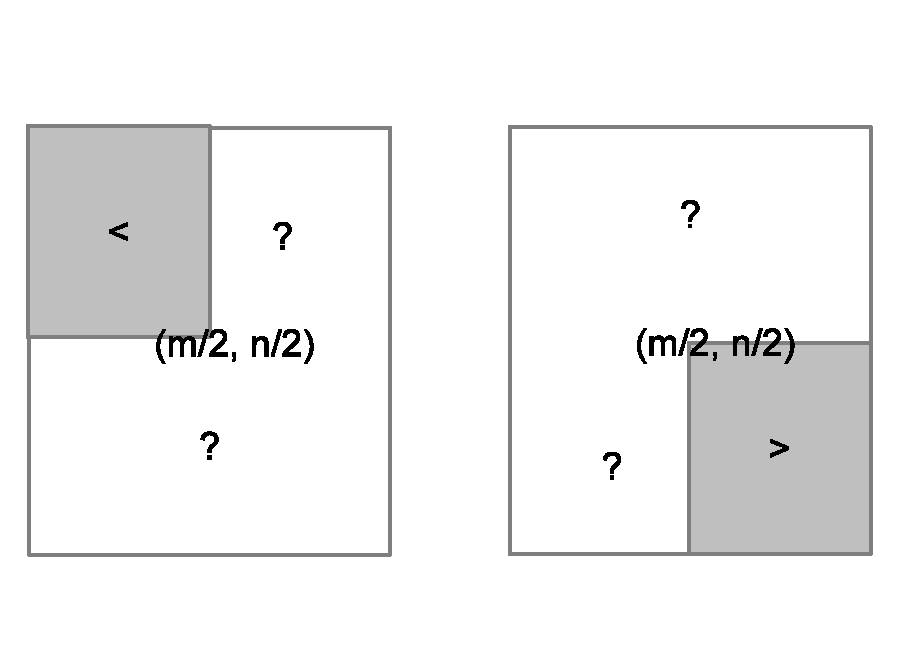
\includegraphics[scale=0.5]{img/bsearch-2D.eps}
 \caption{左:中点的元素小于$x$。所有灰色区域的元素都小于$x$;右:中点的元素大于$x$。所有灰色区域的元素都大于$x$。}
 \label{fig:bsearch-2D}
\end{figure}

这里出现的问题是,两种情况下,搜索区域都从一个矩形变成了一个L形,我们无法继续递归地进行搜索。为了系统化地解决这一问题,我们先给出一个通用的定义,然后从穷举法开始,逐步改进,直到获得满意的答案。

考虑严格单调增函数$f(x, y)$,例如$f(x, y) = a^x + b^y$,其中$a$和$b$都是自然数。给定自然数$z$,我们希望寻找全部的非负整数解$(x, y)$。

使用这一定义,上述的矩阵搜索问题,可以特殊化为下面的函数:

\[
f(x, y) = \left \{
  \begin{array}
  {r@{\quad:\quad}l}
  M_{x, y} & 1 \leq x \leq m, 1 \leq y \leq n \\
  -1 & otherwise
  \end{array}
\right.
\]

\paragraph{穷举法二维搜索}

既然要找出$f(x, y)$的所有解,最简单的方法就是双重循环的穷举法:

\begin{algorithmic}[1]
\Function{Solve}{$f, z$}
  \State $A \gets \phi$
  \For{$x \in \{0, 1, 2, ..., z\}$}
    \For{$y \in \{0, 1, 2, ..., z\}$}
      \If{$f(x, y) = z$}
        \State $A \gets A \cup \{(x, y)\}$
      \EndIf
    \EndFor
  \EndFor
  \State \Return $A$
\EndFunction
\end{algorithmic}

显然,这一方法计算了$(z+1)^2$次$f$。它可以形式化为式(\ref{eq:bsearch-brute})的定义:

\be
solve(f, z) = \{ (x, y) | x \in \{0, 1, ..., z\}, y \in \{0, 1, ..., z\}, f(x, y) = z\}
\label{eq:bsearch-brute}
\ee

\paragraph{Saddleback搜索}
\index{Saddelback搜索}

我们尚未使用$f(x, y)$为严格单调增的条件。Dijkstra指出\cite{saddle-back},有效的解法不是从左下角出发,而是从左上角出发开始查找。如图\ref{fig:saddleback-1}所示,搜索从$(0, z)$开始,对于每个点$(p, q)$,我们比较$f(p q)$和$z$的关系:

\begin{itemize}
\item 如果$f(p, q) < z$,由于$f$单调增,对于所有的$0 \leq y < q$,必然有$f(p, y) < z$。我们可以丢弃垂直线段上的所有点(红色线段);
\item 如果$f(p, q) > z$,则对于所有的$p < x \leq z$,必然有$f(x, q) > z$。我们可以丢弃水平线段上的所有点(蓝色线段);
\item 否则,若$f(p, q) = z$,则$(p, q)$是一个解,两条线段上的点都可以丢弃。
\end{itemize}

这样,我们就可以逐步缩小矩形的搜索区域。每次要么丢弃一行,要么丢弃一列,或者同时丢弃行和列。

\begin{figure}[htbp]
 \centering
 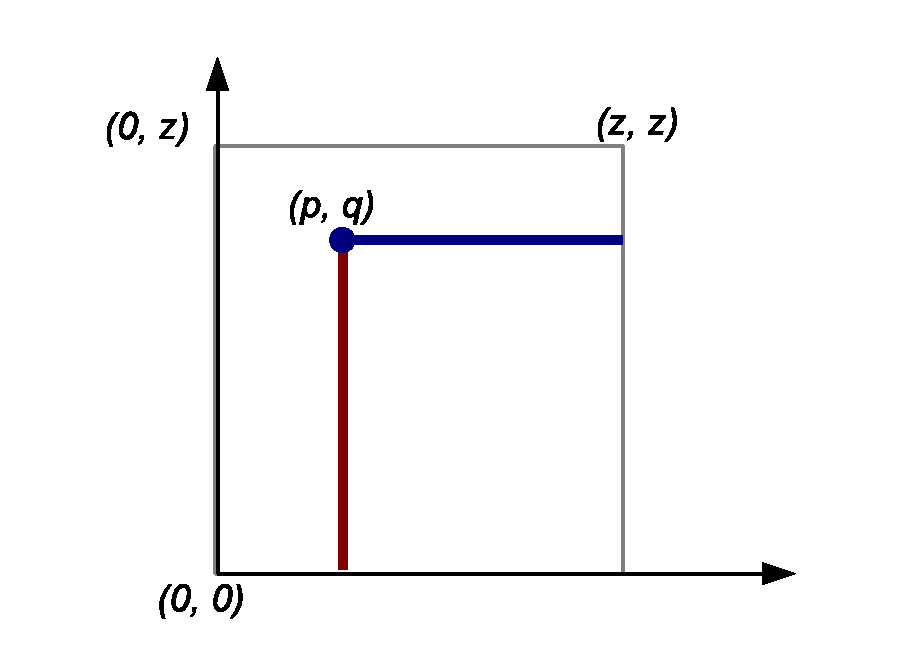
\includegraphics[scale=0.5]{img/saddleback-1.eps}
 \caption{从左上角搜索。}
 \label{fig:saddleback-1}
\end{figure}

这一方法可以定义为一个函数$search(f, z, p, q)$,它在矩形区域内搜索方程$f(x, y) = z$的整数解,矩形的左上角为$(p, q)$,右下角为$(z, 0)$。这个矩形的左上角一开始时为$(p, q) = (0, z)$,然后启动搜索$solve(f, z) = search(f, z, 0, z)$。

\be
search(f, z, p, q) =  \left \{
  \begin{array}
  {r@{\quad:\quad}l}
  \phi & p > z \lor q < 0 \\
  search(f, z, p + 1, q) & f(p, q) < z \\
  search(f, z, p, q - 1) & f(p, q) > z \\
  \{(p, q)\} \cup search(f, z, p + 1, q - 1) & otherwise
  \end{array}
\right.
\ee

第一行为边界条件,如果$(p q)$不再$(z, 0)$的左上方,则无解。下面的Haskell例子程序实现了这一算法:

\lstset{language=Haskell}
\begin{lstlisting}
solve f z = search 0 z where
  search p q | p > z || q < 0 = []
             | z' < z = search (p + 1) q
             | z' > z = search p (q - 1)
             | otherwise = (p, q) : search (p + 1) (q - 1)
    where z' = f p q
\end{lstlisting}

考虑到计算$f$的过程消耗可能较大,这一程序将计算结果$f(p, q)$存储在变量$z'$中。算法也可以用imperative的方式实现,在循环中不断更新搜索区域的边界。

\begin{algorithmic}[1]
\Function{Solve}{$f, z$}
  \State $p \gets 0, q \gets z$
  \State $S \gets \phi$
  \While{$p \leq z \land q \geq 0$}
    \State $z' \gets f(p, q)$
    \If{$z' < z$}
      \State $p \gets p + 1$
    \ElsIf{$z' > z$}
      \State $q \gets q - 1$
    \Else
      \State $S \gets S \cup \{(p, q)\}$
      \State $p \gets p + 1, q \gets q - 1$
    \EndIf
  \EndWhile
  \State \Return $S$
\EndFunction
\end{algorithmic}

下面的Python例子程序实现了这一算法。

\lstset{language=Python}
\begin{lstlisting}
def solve(f, z):
    (p, q) = (0, z)
    res = []
    while p <= z and q >= 0:
        z1 = f(p, q)
        if z1 < z:
            p = p + 1
        elif z1 > z:
            q = q - 1
        else:
            res.append((p, q))
            (p, q) = (p + 1, q - 1)
    return res

\end{lstlisting}

显然在每次迭代中,$p$和$q$中至少有一个会向右下角前进一步。因此最多需要$2(z+1)$次迭代以完成搜索。这是最差情况下的结果。最好的情况又分为三种,第一种是每次迭代$p$和$q$同时前进一步,因此只需要$z+1$步就可以完成搜索;第二种是不断沿着水平方向向右前进,最后$p$超过$z$;第三种与此类似,不断沿着垂直方向向下前进,最终$q$变为负。

图\ref{fig:saddleback-1-cases}描述了最好和最坏的情况。图\ref{fig:saddleback-1-cases} (a)中,对角线上的每个点$(x, z-x)$都满足$f(x, z-x) = z$,总共需要$z+1$步到达$(z, 0)$;(b)中,最上不水平线上的每个点$(x, z)$都使得$f(x, z) < z$,$z+1$步后,搜索结束;(c)中,左侧垂直线上的每个点$(0, x)$都使得$f(0, x) > z$,因此$z+1$步后,搜索结束;(d)描述的是最差情况。如果我们将搜索路径上的所有水平线段投射$x$轴上,所有垂直线段投射到$y$轴上,就可以得到总共的搜索步数为$2(z+1)$。

\begin{figure}[htbp]
 \centering
 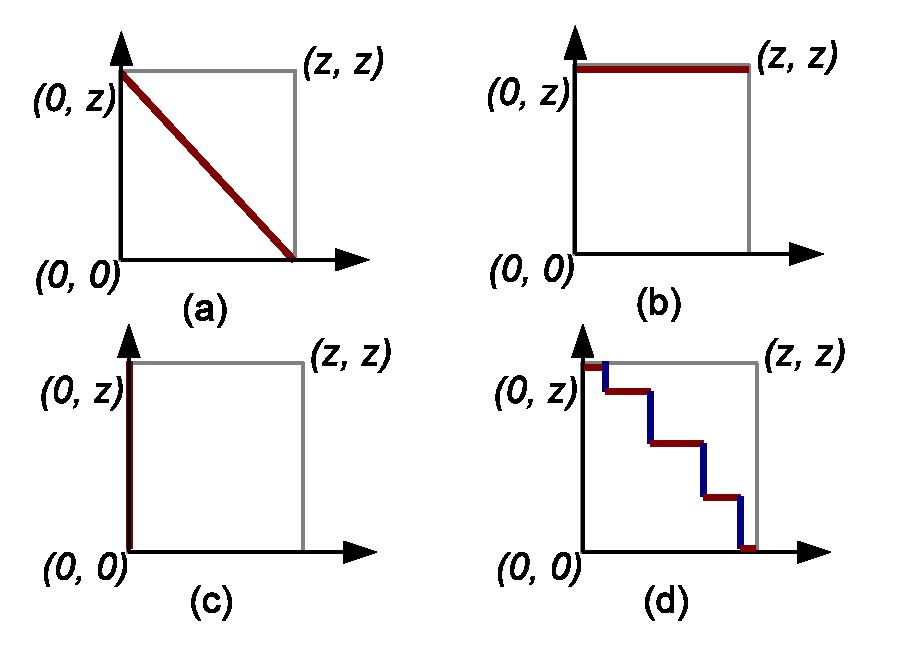
\includegraphics[scale=0.5]{img/saddleback-1-cases.eps}
 \caption{最好和最差情况。}
 \label{fig:saddleback-1-cases}
\end{figure}

和复杂度为$O(z^2)$的穷举法相比,这一改进将复杂度提高到线性时间$O(z)$。

Bird猜测,这一算法的名称saddleback的由来是因为函数$f$的3维图像中,左下部的最小值和右上部的最大值,以及两侧的翼形图像,合起来像一个马鞍。如图\ref{fig:saddleback-frame}所示。

\begin{figure}[htbp]
 \centering
 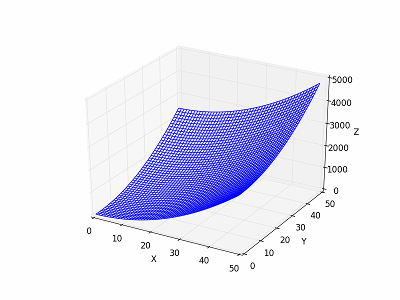
\includegraphics[scale=0.8]{img/saddleback-xx-yy.eps}
 \caption{函数$f(x, y) = x^2 + y^2$的图像。}
 \label{fig:saddleback-frame}
\end{figure}

\paragraph{改进的saddleback搜索}

问题扩展到2维后,我们尚未使用二分查找来改进算法。基本的saddleback搜索从左上角$(0, z)$开始,向右下角$(z, 0)$进行搜索。这一范围实可以进一步缩小。

因为$f$单调增,我们可以沿着$y$轴找到最大的$m$,使得$0 \leq m \leq z$且$f(0, m) \leq z$;同样,我们可以沿着$x$轴找到最大的$n$,使得$0 \leq n \leq z$且$f(n, 0) \leq z$;这样搜索区域就从 原来的$(0, z) - (z, 0)$缩小到$(0, m) - (n, 0)$,如图\ref{fig:saddleback-2}所示。

\begin{figure}[htbp]
 \centering
 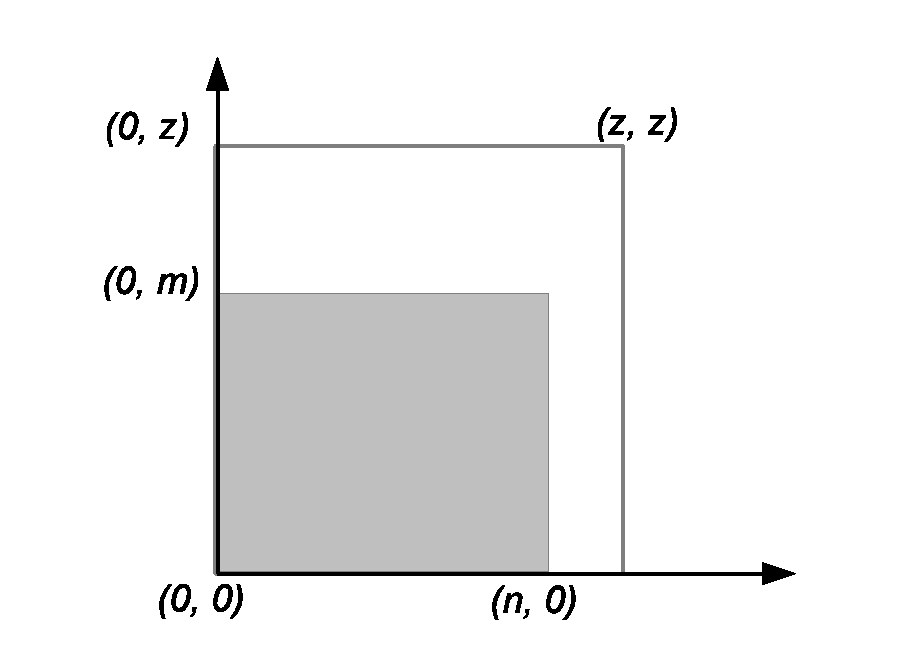
\includegraphics[scale=0.5]{img/saddleback-2.eps}
 \caption{缩小的灰色搜索区域。}
 \label{fig:saddleback-2}
\end{figure}

显然$m$和$n$可用穷举法找到:

\be
\begin{array}{rl}
m & = max(\{y | 0 \leq y \leq z, f(0, y) \leq z\}) \\
n & = max(\{x | 0 \leq x \leq z, f(x, 0) \leq z\})
\end{array}
\ee

当搜索$m$时,函数$f$的变量$x$固定为0。这就转化为了一维的单调增函数搜索问题(在函数式环境中,称为Curried化函数$f(0, y)$)。可以使用二分查找来改进这一搜索。但是我们需要对式(\ref{eq:bsearch})略加改动。给定$y$,我们不是要寻找$l \leq x \leq u$,使得$f(x) = y$。而是要寻找$l \leq x \leq u$使得满足不等式$f(x) \leq y < f(x+1)$。

\be
bsearch(f, y, l, u) = \left \{
  \begin{array}
  {r@{\quad:\quad}l}
  l & u \leq l \\
  m & f(m) \leq y < f(m+1), m = \lfloor \frac{l + u}{2} \rfloor \\
  bsearch(f, y, m + 1, u) & f(m) \leq y \\
  bsearch(f, y, l, m-1) & otherwise
  \end{array}
\right.
\label{eq:bsearch-general}
\ee

第一行处理搜索区域为空的边界情况,此时我们返回搜索区域的下界;如果中点对应的函数值小于等于$y$,而下一个值对应的函数值大于$y$,则中点就是我们要搜索的结果;否则,如果中点下一个值对应的函数值也不大于$y$,就将中点的下一个值作为新的下届,递归地进行二分查找;最后,如果中点对应的函数值大于$y$,则用中点前的一个值作为新的上界,递归进行查找。下面的Haskell例子程序实现了这样的二分查找。

\lstset{language=Haskell}
\begin{lstlisting}
bsearch f y (l, u) | u <= l = l
                   | f m <= y = if f (m + 1) <= y
                                then bsearch f y (m + 1, u) else m
                   | otherwise = bsearch f y (l, m-1)
  where m = (l + u) `div` 2
\end{lstlisting}

这样,$m$和$n$可以使用二分查找来确定:

\be
\begin{array}{rl}
m & = bsearch(\lambda_y \cdot f(0, y), z, 0, z) \\
n & = bsearch(\lambda_x \cdot f(x, 0), z, 0, z)
\end{array}
\label{eq:bsearch-boundaries}
\ee

我们可以将saddleback搜索的区域缩小为更精确的矩形$solve(f, z) = search(f, z, 0, m)$:

\be
search(f, z, p, q) =  \left \{
  \begin{array}
  {r@{\quad:\quad}l}
  \phi & p > n \lor q < 0 \\
  search(f, z, p + 1, q) & f(p, q) < z \\
  search(f, z, p, q - 1) & f(p, q) > z \\
  \{(p, q)\} \cup search(f, z, p + 1, q - 1) & otherwise
  \end{array}
\right.
\ee

大部分和基本的saddleback一样,但是当$p$超过$n$的时候,就可以停止,而无需达到$z$。在实际的实现中,可以将$f(p, q)$的值保存下来,而不用每次计算。如下面的Haskell例子代码所示:

\lstset{language=Haskell}
\begin{lstlisting}
solve' f z = search 0 m where
  search p q | p > n || q < 0 = []
             | z' < z = search (p + 1) q
             | z' > z = search p (q - 1)
             | otherwise = (p, q) : search (p + 1) (q - 1)
    where z' = f p q
  m = bsearch (f 0) z (0, z)
  n = bsearch (\x->f x 0) z (0, z)
\end{lstlisting}

这一改进的saddleback搜索,首先使用两轮二分查找得到$m$和$n$。每轮二分查找都计算了$O(\lg z)$次$f$;此后,算法在最坏情况下计算$O(m+n)$次;而在最好的情况下计算$O(min(m, n))$次。总体的性能如下表所示:

\begin{tabular}{|l|l|}
\hline
 & 计算$f$的次数 \\
\hline
最坏情况 & $2 \log z + m + n$ \\
最好情况 & $2 \log z + min(m, n)$ \\
\hline
\end{tabular}

某些函数,例如$f(x, y) = a^x + b^y$,对于正整数$a$和$b$,$m$和$n$相对很小,因此整体性能接近$O(\lg z)$。

这一算法也可以用命令式的方法实现。首先需要修改命令式的二分查找算法:

\begin{algorithmic}[1]
\Function{Binary-Search}{$f, y, (l, u)$}
  \While{$l < u$}
    \State $m \gets \lfloor \frac{l + u}{2} \rfloor$
    \If{$f(m) \leq y$}
      \If{$y < f(m+1)$}
        \State \Return m
      \EndIf
      \State $l \gets m + 1$
    \Else
      \State $u \gets m$
    \EndIf
  \EndWhile
  \State \Return $l$
\EndFunction
\end{algorithmic}

使用上述二分查找,在开始saddleback搜索前,先确定$m$和$n$。

\begin{algorithmic}[1]
\Function{Solve}{$f, z$}
  \State $m \gets$ \Call{Binary-Search}{$\lambda_y \cdot f(0, y), z, (0, z)$}
  \State $n \gets$ \Call{Binary-Search}{$\lambda_x \cdot f(x, 0), z, (0, z)$}
  \State $p \gets 0, q \gets m$
  \State $S \gets \phi$
  \While{$p \leq n \land q \geq 0$}
    \State $z' \gets f(p, q)$
    \If{$z' < z$}
      \State $p \gets p + 1$
    \ElsIf{$z' > z$}
      \State $q \gets q - 1$
    \Else
      \State $S \gets S \cup \{(p, q)\}$
      \State $p \gets p + 1, q \gets q - 1$
    \EndIf
  \EndWhile
  \State \Return $S$
\EndFunction
\end{algorithmic}

具体的实现留给读者作为练习。

\paragraph{Saddleback搜索的进一步改进}

图\ref{fig:bsearch-2D}展示的两种情况中,矩阵中点的值要么比目标值小,要么比目标值大。都只能丢弃$\frac{1}{4}$区域中的元素,而剩余的搜索区域变为一个L形。

事实上,我们忽略了另外的一个重要情况。我们观察矩形搜索区域中的任一一点,如图\ref{fig:saddleback-drop}所示。

\begin{figure}[htbp]
 \centering
 \subfloat[如果$f(p, q) \neq z$,只能丢弃左下或右上的区域(灰色部分)。两种情况下,剩余的搜索区域都变成了L形。]{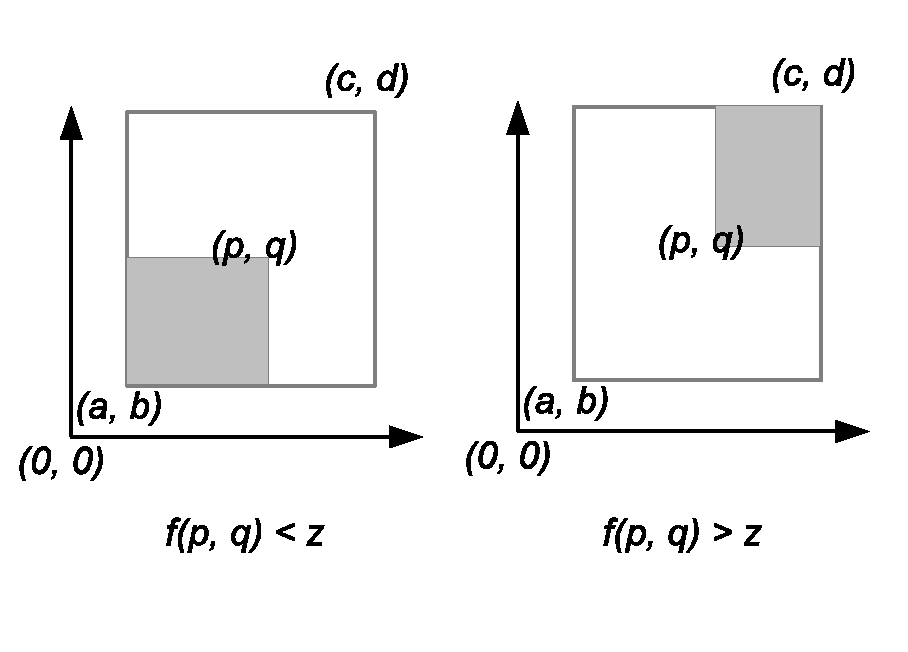
\includegraphics[scale=0.5]{img/saddleback-3.eps}} \\
 \subfloat[如果$f(p, q) = z$,可以同时丢弃两个子区域,问题的搜索域减半。]{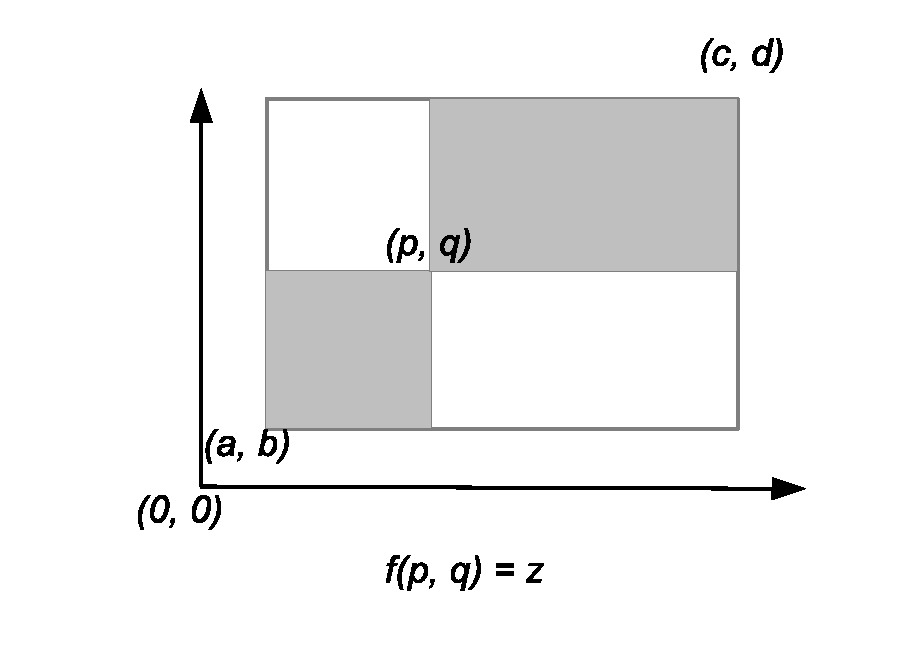
\includegraphics[scale=0.5]{img/saddleback-4.eps}}
 \caption{缩小搜索区域的效率。}
 \label{fig:saddleback-drop}
\end{figure}

考虑搜索一个矩形区域,左下角为$(a, b)$,右上角为$(c, d)$。如果$(p, q)$不是矩形的中点,并且$f(p, q) \neq z$,我们并不能保证被丢弃的部分总是1/4。但是,如果$f(p, q) = z$,由于$f$是单调增的,我们可以同时丢弃左下和右上的子区域,并且$p$列和$q$行上的所有其他点也都可以丢弃掉。这样每次只剩下1/2的区域,可以迅速缩小搜索的区间。

由此可知,我们无需找到矩形的中点进行搜索。更有效的方法是找到函数值等于目标值的点。我们可以沿着矩形中心的水平方向或者垂直方向使用二分查找来定位这样的点。

在线段上进行二分查找的性能和线段的长度成对数关系。我们可以选取水平和垂直方向中较短的中线进行搜索,如图\ref{fig:saddleback-centerline}所示。

\begin{figure}[htbp]
 \centering
 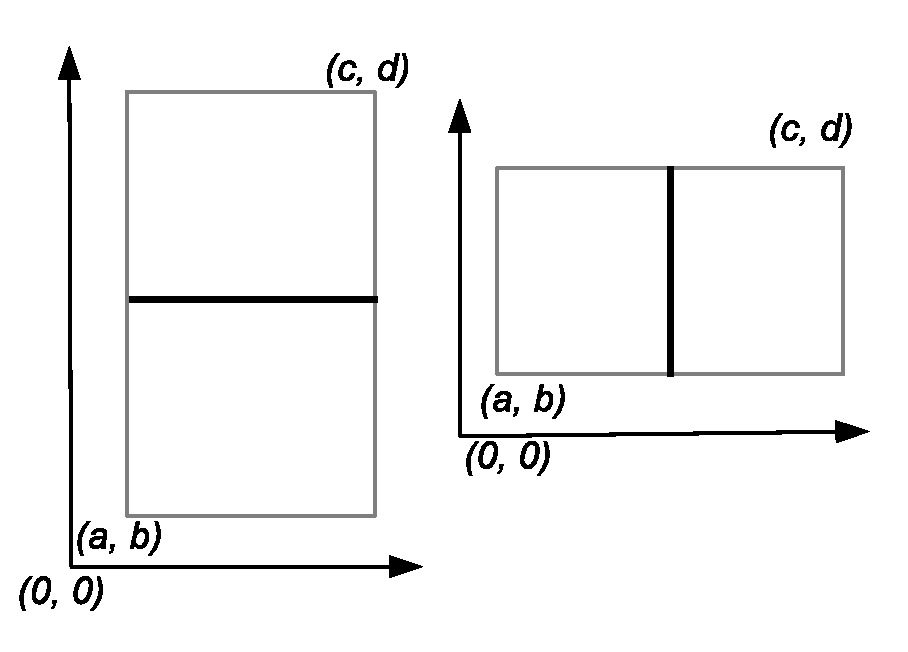
\includegraphics[scale=0.5]{img/saddleback-centerline.eps}
 \caption{沿较短的中线进行二分查找。}
 \label{fig:saddleback-centerline}
\end{figure}

但是,如果中线行不存在满足$(p, q) = z$的点时如何处理呢?例如,水平中线上不存在这样的点。此时,我们仍然能够找到一点满足$f(p, q) < z < f(p+1, q)$。唯一不同之处是我们不能将$p$列和$q$行上的点完全丢弃。

综合上述情况,沿着水平线二分搜索以要找到一点$p$,其满足件$f(p, q) \leq z < f(p+1, q)$;而沿着垂直线二分搜索的条件是$f(p, q) \leq z < f(p, q + 1)$。

如果线段上所有的点都使得$f(p, q) < z$,则修改后的二分查找会返回上界作为结果;反之,如果所有点对应的函数值都大于$z$,则返回下届作为结果。此时,我们可以将中线一侧的整个区域全部丢弃。

总结这些结论,我们可以给出下面的改进saddleback搜索算法:

\begin{enumerate}
\item 沿着$y$轴和$x$轴进行二分搜索,定位出搜索区域的边界,从$(0, m)$到$(n, 0)$;
\item 记待搜索的矩形区域为$(a, b) - (c, d)$,若矩形为空,则无解;
\item 若矩形的高大于宽,则沿着水平中线进行二分查找;否则,沿着垂直中线进行二分查找;记查找的结果为点$(p, q)$;
\item 若$f(p, q) = z$,记录$(p, q)$为一个解,然后递归搜索两个子矩形区域$(a, b) - (p-1, q+1)$和$(p+1, q-1) - (c, d)$;
\item 否则,若$f(p, q) \neq z$,递归搜索同样的两个子矩形区域和一条线段。线段或者为$(p, q+1) - (p, b)$如图\ref{fig:include-line} (a);或者为$(p+1, q) - (c, q)$如图\ref{fig:include-line} (b)。
\end{enumerate}

\begin{figure}[htbp]
 \centering
 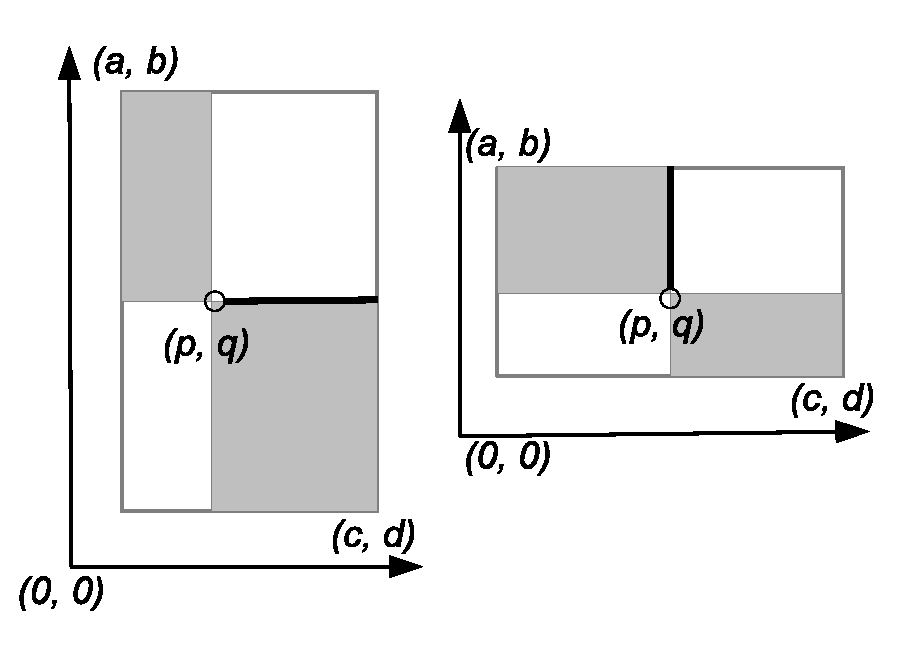
\includegraphics[scale=0.5]{img/saddleback-include-ln.eps}
 \caption{递归搜索灰色的区域,如果$f(p, q) \neq z$,还需要搜索加粗的线段。}
 \label{fig:include-line}
\end{figure}

我们复用前面式(\ref{eq:bsearch-general})和(\ref{eq:bsearch-boundaries})的定义。定义$Search_{(a, b), (c, d)}$为新的搜索函数,它搜索一个矩形区域,其中左上角为$(a, b)$,右下角为$(c, d)$。

\be
search_{(a, b), (c, d)} =  \left \{
  \begin{array}
  {r@{\quad:\quad}l}
  \phi & c < a \lor d < b \\
  csearch & c - a < b - d \\
  rsearch & otherwise
  \end{array}
\right.
\ee

函数$csearch$在水平中线上进行二分查找,寻找一点$(p, q)$使得$f(p, q) \leq z < f(p+1, q)$。如图\ref{fig:include-line} (a)所示。如果中线上所有点对应的函数值都大于$z$,二分查找返回下界作为结果,即$(p, q) = (a, \lfloor \frac{b + d}{2} \rfloor)$。中线和它上侧的区域全部可以丢弃,如图\ref{fig:saddleback-edge-cases} (a).所示。

\begin{figure}[htbp]
 \centering
 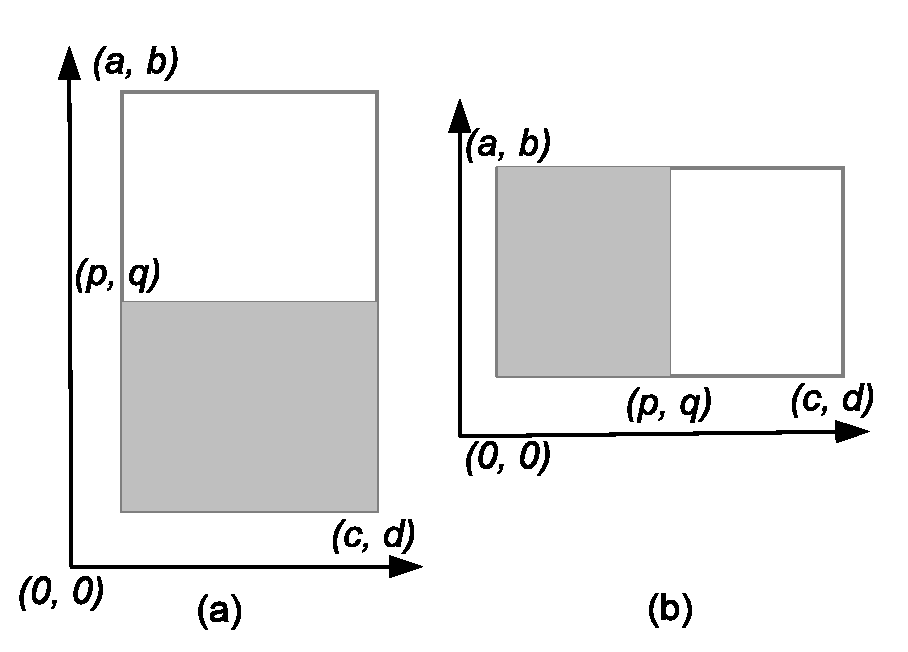
\includegraphics[scale=0.5]{img/saddleback-edge-cases.eps}
 \caption{沿中线进行二分查找时的特殊情况。}
 \label{fig:saddleback-edge-cases}
\end{figure}

\be
csearch = \left \{
  \begin{array}
  {r@{\quad:\quad}l}
  search_{(p, q-1), (c, d)} & z < f(p, q) \\
  search_{(a, b), (p-1, q+1)} \cup \{(p, q)\} \cup search_{(p+1, q-1), (c, d)} & f(p, q) = z \\
  search_{(a, b), (p, q+1)} \cup search_{(p+1, q-1), (c, d)} & otherwise
  \end{array}
\right.
\ee

其中

\[
\begin{array}{l}
q = \lfloor \frac{b + d}{2} \rfloor) \\
p = bsearch(\lambda_x \cdot f(x, q), z, (a, c))
\end{array}
\]

函数$rsearch$与此类似,它沿着垂直中线进行搜索。

\be
rsearch = \left \{
  \begin{array}
  {r@{\quad:\quad}l}
  search_{(a, b), (p - 1, q)} & z < f(p, q) \\
  search_{(a, b), (p-1, q+1)} \cup \{(p, q)\} \cup search_{(p+1, q-1), (c, d)} & f(p, q) = z \\
  search_{(a, b), (p-1, q+1)} \cup search_{(p+1, q), (c, d)} & otherwise
  \end{array}
\right.
\ee

其中

\[
\begin{array}{l}
p = \lfloor \frac{a + c}{2} \rfloor) \\
q = bsearch(\lambda_y \cdot f(p, y), z, (d, b))
\end{array}
\]

下面的Haskell例子程序实现了这一算法。

\lstset{language=Haskell}
\begin{lstlisting}
search f z (a, b) (c, d) | c < a || b < d = []
                         | c - a < b - d = let q = (b + d) `div` 2 in
                                             csearch (bsearch (\x -> f x q) z (a, c), q)
                         | otherwise = let p = (a + c) `div` 2 in
                                             rsearch (p, bsearch (f p) z (d, b))
  where
    csearch (p, q) | z < f p q = search f z (p, q - 1) (c, d)
                   | f p q == z = search f z (a, b) (p - 1, q + 1) ++
                                    (p, q) : search f z (p + 1, q - 1) (c, d)
                   | otherwise = search f z (a, b) (p, q + 1) ++
                                   search f z (p + 1, q - 1) (c, d)
    rsearch (p, q) | z < f p q = search f z (a, b) (p - 1, q)
                   | f p q == z = search f z (a, b) (p - 1, q + 1) ++
                                    (p, q) : search f z (p + 1, q - 1) (c, d)
                   | otherwise = search f z (a, b) (p - 1, q + 1) ++
                                    search f z (p + 1, q) (c, d)
\end{lstlisting}

主程序首先沿着$X$轴和$Y$轴进行二分查找,然后调用上述函数。

\lstset{language=Haskell}
\begin{lstlisting}
solve f z = search f z (0, m) (n, 0) where
  m = bsearch (f 0) z (0, z)
  n = bsearch (\x -> f x 0) z (0, z)
\end{lstlisting}

由于每次都丢弃一半的区域,算法总共搜索$O(\log (mn))$轮搜索。但是,为了寻找点$(p, q)$使得问题规模减半,我们需要沿着中线进行二分查找。这样需要计算$f$的次数为$O(\log min(m, n))$。令在大小为$m \times n$的矩形区域搜索的时间为$T(m, n)$,我们有如下的递归关系:

\be
T(m, n) = \log(min(m, n)) + 2 T(\frac{m}{2}, \frac{n}{2})
\ee

不妨设$m > n$,使用telescope方法,若$m = 2^i$、$n = 2^j$,我们有:

\be
\begin{array}{rl}
T(2^i, 2^j) & = j + 2 T(2^{i-1}, 2^{j-1}) \\
            & = \displaystyle \sum_{k=0}^{i-1} 2^k(j - k) \\
            & = O(2^i(j-i)) \\
            & = O(m \log (n/m))
\end{array}
\ee

Richard Bird证明了,这是在$m \times n$的矩形区域内搜索一给定值的最优下界\cite{fp-pearls}。

命令式的实现与此类似,我们在此将其略过。

\begin{Exercise}
\begin{itemize}
\item 参考前面章节快速排序的部分,证明分而治之的$k$选择算法,在平均情况下的性能为$O(n)$。
\item 使用两路划分和三点中值法实现命令式的$k$选择算法。
\item 实现能有效处理大量重复元素的命令式的$k$选择算法。
\item 选择一门编程语言,实现median-of-median的$k$选择算法。
\item 本节给出的$tops(k, L)$使用了列表的连接操作,如$A \cup \{ l_1 \} \cup tops(k - |A| - 1, B)$。这一操作的性能为线性时间,和被连接列表的长度成比例。修改算法,仅用一遍处理就将子列表连接起来。
\item 作者想出了另外一种分而治之的$k$选择问题解法。首先找到前$k$个元素中的最大值,和剩余元素中的最小值,分别记为$x$和$y$,若$x$小于$y$,说明所有的前$k$个元素都小于剩余的元素,它们恰巧是最小的$k$个元素;否则,说明前$k$个元素中的某些元素,需要被交换到后面去。
\begin{algorithmic}[1]
\Procedure{Tops}{$k, A$}
  \State $l \gets 1$
  \State $u \gets |A|$
  \Loop
    \State $i \gets$ \Call{Max-At}{$A[l..k]$}
    \State $j \gets$ \Call{Min-At}{$A[k+1..u]$}
    \If{$A[i] < A[j]$}
      \State break
    \EndIf
    \State \textproc{Exchange} $A[l] \leftrightarrow A[j]$
    \State \textproc{Exchange} $A[k+1] \leftrightarrow A[i]$
    \State $l \gets$ \Call{Partition}{$A, l, k$}
    \State $u \gets$ \Call{Partition}{$A, k+1, u$}
  \EndLoop
\EndProcedure
\end{algorithmic}
请说明这一算法正确与否?性能如何?
\item 使用迭代的方式和递归的方式分别实现二分查找算法,并使用自动的方式进行测试。可以使用生成的随机测试数据,也可以定义一些不变性质,并和编程环境中内置的二分查找工具对比。
\item 任意给定两个已序数组$A$和$B$,寻找它们的中值(median)。要求时间复杂度为$O(\lg (|A| + |B|))$。
\item 使用一门命令式语言,在进行saddleback搜索前,先通过二分查找定位出更精确的搜索区域。
\item 使用一门命令式语言,沿着较短的中线进行二分查找,从而实现改进的二维搜索。
\item 有人给出了这样的二维搜索算法:当搜索一个矩形区域时,由于左下角是最小值,右上角是最大值。若待搜索的值小于最小值或者大于最大值,则无解;否则,从中点将矩形区域分割成4个小矩形,然后进行递归搜索。
\begin{algorithmic}[1]
\Procedure{Search}{$f, z, a, b, c, d$} \Comment{$(a, b)$:左下角 $(c, d)$:右上角}
  \If {$z \leq f(a, b) \lor f(c, d) \geq z$}
    \If{$z = f(a, b)$}
      \State record $(a, b)$ as a solution
    \EndIf
    \If{$z = f(c, d)$}
      \State record $(c, d)$ as a solution
    \EndIf
    \State \Return
  \EndIf
  \State $p \gets \lfloor \frac{a + c}{2} \rfloor$
  \State $q \gets \lfloor \frac{b + d}{2} \rfloor$
  \State \Call{Search}{$f, z, a, q, p, d$}
  \State \Call{Search}{$f, z, p, q, c, d$}
  \State \Call{Search}{$f, z, a, b, p, q$}
  \State \Call{Search}{$f, z, p, b, c, q$}
\EndProcedure
\end{algorithmic}
试分析这一算法的性能。
\end{itemize}
\end{Exercise}

\subsection{信息复用}

人会通过搜索来学习。我们不仅记忆搜索失败的教训,还学习总结成功的模式。这是某种意义上的信息复用,不论这些信息是正面的还是负面的。但难点在于决定记忆哪些信息。记忆太少的信息不足以提高搜索的效率,记忆太多的信息又无法满足存储空间的限制。

本节我们首先介绍两个有趣的问题:Boyer-Moore众数(majority number)问题,和子数组最大和问题。它们都通过复用最少的信息来解决问题。然后,我们介绍两种被广泛使用的字符串匹配算法:KMP(Knuth-Morris-Pratt)算法,和Boyer-Moore算法。

\subsubsection{Boyer-Moore众数问题}
\index{Boyer-Moor众数问题}

人们常常通过投票来进行一些决策,例如选举领袖,接受或者拒绝一项建议。在作者写作本章的时候,有三个国家正在通过投票选举总统,他们都使用计算机来统计投票结果。

假设某个小岛上的国家要通过投票选出新的总统。这个国家的宪法规定,只有赢得半数以上选票的人才可以成为总统。从一个投票结果的序列,例如A, B, A, C, B, B, D, ...我们能否找到一种高效的方法,得知谁当选了总统,或者没有任何人赢得半数以上的选票?

显然可以通过使用一个map,然后遍历一遍选票来解决这个问题。如我们在二叉搜索树一章给出例子那样\footnote{2004年,人们发现了一种概率算法,称为Count-min sketch算法,使用sub-linear空间进行计数\cite{count-min-sketch}。}

\lstset{language=C++}
\begin{lstlisting}
template<typename T>
T majority(const T* xs, int n, T fail) {
    map<T, int> m;
    int i, max = 0;
    T r;
    for (i = 0; i < n; ++i)
        ++m[xs[i]];
    for (typename map<T, int>::iterator it = m.begin(); it != m.end(); ++it)
        if (it->second > max) {
            max = it->second;
            r = it->first;
        }
    return max * 2 > n ? r : fail;
}
\end{lstlisting}

这段例子程序首先扫描所有选票,然后通过map累计所有候选人的票数。接着,他遍历map找到得票最多的候选人。若票数超过半数,则此人获胜,否则程序返回一个特殊值表示无人获胜。

下面的伪代码描述了这一算法。

\begin{algorithmic}[1]
\Function{Majority}{$A$}
  \State $M \gets $ empty map
  \For{$\forall a \in A$}
    \State \textproc{Put}($M$, $a, 1 + $ \Call{Get}{$M, a$})
  \EndFor
  \State $max \gets 0$, $m \gets NIL$
  \For{$\forall (k, v) \in M$}
    \If{$max < v$}
      \State $max \gets v$, $m \gets k$
    \EndIf
  \EndFor
  \If{$max > |A| 50\%$}
    \State \Return $m$
  \Else
    \State fail
  \EndIf
\EndFunction
\end{algorithmic}

对于$m$名候选人和$n$张选票,若使用自平衡树实现的map(如红黑树map),这一程序首先需要$O(n \log m)$时间来构建map;若使用Hash表实现的map,则所用时间为$O(n)$。但是Hash表所用的空间会更多。接下来,程序需要$O(m)$的时间来遍历map,然后寻找票数最多的候选人。下表给出了使用不同种类map所需的时间和空间的对比。

\begin{tabular}{|l|l|l|}
\hline
map & 时间 & 空间 \\
\hline
自平衡树 & $O(n \log m)$ & $O(m)$ \\
hashing & $O(n)$ & 最少$O(m)$ \\
\hline
\end{tabular}

Boyer和Moore在1980年发现了一种巧妙的方法,如果存在超过半数的元素,可以只扫描一遍就找到它。并且这一方法只需要$O(1)$的空间\cite{boyer-moore-majority}。

首先我们记录第一张选票投给的候选人为目前的获胜者,所赢得票数为1。在接下来的扫描中,若下一张选票还投给目前的获胜者,就将获胜者的票数加1;否则,下一张选票没有投给目前的获胜者,我们将获胜者的赢得的票数减1。若获胜者的净赢得的票数变为0,说明他不再是获胜者了,我们选择下一张选票上的候选人作为新的获胜者,并继续重复这一扫描过程。

假设选票的序列为:A, B, C, B, B, C, A, B, A, B, B, D, B。下表给出了这一扫描处理的各个步骤。

\begin{tabular}{|l|l|l|}
\hline
获胜者 & 净赢票数 & 扫描位置 \\
\hline
A & 1 & \underline{A}, B, C, B, B, C, A, B, A, B, B, D, B \\
A & 0 & A, \underline{B}, C, B, B, C, A, B, A, B, B, D, B \\
C & 1 & A, B, \underline{C}, B, B, C, A, B, A, B, B, D, B \\
C & 0 & A, B, C, \underline{B}, B, C, A, B, A, B, B, D, B \\
B & 1 & A, B, C, B, \underline{B}, C, A, B, A, B, B, D, B \\
B & 0 & A, B, C, B, B, \underline{C}, A, B, A, B, B, D, B \\
A & 1 & A, B, C, B, B, C, \underline{A}, B, A, B, B, D, B \\
A & 0 & A, B, C, B, B, C, A, \underline{B}, A, B, B, D, B \\
A & 1 & A, B, C, B, B, C, A, B, \underline{A}, B, B, D, B \\
A & 0 & A, B, C, B, B, C, A, B, A, \underline{B}, B, D, B \\
B & 1 & A, B, C, B, B, C, A, B, A, B, \underline{B}, D, B \\
B & 0 & A, B, C, B, B, C, A, B, A, B, B, \underline{D}, B \\
B & 1 & A, B, C, B, B, C, A, B, A, B, B, D, \underline{B} \\
\hline
\end{tabular}

这里关键的一点是:若存在一个超过50\%的众数,则它不可能被其它元素超越落选。但是,如果没有任何候选者赢得半数以上的选票,则最后所记录的“获胜者”并无意义。此时需要再进行一轮扫描进行验证。

下面的算法实现了这一思路。

\begin{algorithmic}[1]
\Function{Majority}{$A$}
  \State $c \gets 0$
  \For{$i \gets$ 1 to $|A|$}
    \If{$c = 0$}
      \State $x \gets A[i]$
    \EndIf
    \If{$A[i] = x$}
      \State $c \gets c + 1$
    \Else
      \State $c \gets c - 1$
    \EndIf
  \EndFor
  \State \Return $x$
\EndFunction
\end{algorithmic}

若存在众数,这一算法首先扫描所有的选票。每扫描一张票,它根据此选票是支持还是反对当前的结果来增减获胜者的净赢票数。若净赢票数变为0,表明当前的获胜者已落选,算法记录下一张选票投给的候选人为新的获胜者,并继续扫描。

这一过程是线性时间$O(n)$的,所用空间仅仅是两个变量。一个用以记录当前的获胜者,另一个记录净赢得的票数。

当众数存在是,虽然上述算法可以将它找出。但当不存在众数时,这一算法仍会输出一个不正确的结果。下面的改进通过增加一轮扫描来进行验证。

\begin{algorithmic}[1]
\Function{Majority}{$A$}
  \State $c \gets 0$
  \For{$i \gets$ 1 to $|A|$}
    \If{$c = 0$}
      \State $x \gets A[i]$
    \EndIf
    \If{$A[i] = x$}
      \State $c \gets c + 1$
    \Else
      \State $c \gets c - 1$
    \EndIf
  \EndFor
  \State $c \gets 0$
  \For{$i \gets 1$ to $|A|$}
    \If{$A[i] = x$}
      \State $c \gets c + 1$
    \EndIf
  \EndFor
  \If{$c > \%50|A|$}
    \State \Return $x$
  \Else
    \State fail
  \EndIf
\EndFunction
\end{algorithmic}

即使增加了验证的过程,这一算法的时间复杂度仍按为$O(n)$,并且所用空间为常数。下面的C++例子程序实现了这一算法\footnote{这是一个更加类似C语言例子,我们只是使用了C++的模板来抽象元素的类型。}。

\lstset{language=C++}
\begin{lstlisting}
template<typename T>
T majority(const T* xs, int n, T fail) {
    T m;
    int i, c;
    for (i = 0, c = 0; i < n; ++i) {
        if (!c)
            m = xs[i];
        c += xs[i] == m ? 1 : -1;
    }
    for (i = 0, c = 0; i < n; ++i, c += xs[i] == m);
    return c * 2 > n ? m : fail;
}
\end{lstlisting}

Boyer-Moore众数算法也可以用纯函数的方式实现。我们不再使用变量来记录和更新信息,而是使用累积(accumulator)的方法。定义核心算法的函数为$maj(c, n, L)$,它接受一个选票列表$L$,目前的获胜者$c$,和净赢得的票数$n$。若选票列表不为空,则$c$在开始的时候为第一张选票的结果$l_1$,净赢得的票数为1,即$maj(l_1, 1, L')$,其中$L'$是除$l_1$以外的剩余选票。下面是这个函数的详细定义:

\be
maj(c, n, L) = \left \{
  \begin{array}
  {r@{\quad:\quad}l}
  c & L = \phi \\
  maj(c, n + 1, L') & l_1 = c \\
  maj(l_1, 1, L') & n = 0 \land l_1 \neq c \\
  maj(c, n - 1, L') & otherwise
  \end{array}
\right.
\ee

我们还需要定义一个函数来验证所得的结果是否超过半数。最终的算法首先检查选票列表,若为空,则不存在众数,否则它通过Boyer-Moore算法找到一个结果$c$,然后再扫描一遍选票列表计算$c$总共赢得的选票是否过半。

\be
majority(L) = \left \{
  \begin{array}
  {r@{\quad:\quad}l}
  fail & L = \phi \\
  c & c = maj(l_1, 1, L'), |\{x | x \in L, x = c\}| > \%50 |L| \\
  fail & otherwise
  \end{array}
\right.
\ee

下面的Haskell例子程序实现了这一算法。

\lstset{language=Haskell}
\begin{lstlisting}
majority :: (Eq a) => [a] -> Maybe a
majority [] = Nothing
majority (x:xs) = let m = maj x 1 xs in verify m (x:xs)

maj c n [] = c
maj c n (x:xs) | c == x = maj c (n+1) xs
               | n == 0 = maj x 1 xs
               | otherwise = maj c (n-1) xs

verify m xs = if 2 * (length $ filter (==m) xs) > length xs
              then Just m else Nothing
\end{lstlisting} %$

\subsubsection{最大子序列和}
\index{最大和问题}

Jon Bentley给出过另一个类似的趣题\cite{programming-pearls}。给定一个序列,如何找出它的子序列和的最大值?例如,下表所示的序列中,子序列\{19, -12, 1, 9, 18\}的和最大,为35。

\begin{tabular}{|c|c|c|c|c|c|c|c|c|c|}
\hline
3 & -13 & 19 & -12 & 1 & 9 & 18 & -16 & 15 & -15 \\
\hline
\end{tabular}

这里,我们只要找出最大和的值。如果所有元素都是整数,显然答案就是全部元素的和。另外一个特殊情况是所有元素都是负数。我们定义空序列的最大和是0。

最简单的方法是穷举:计算出所有子序列的和,然后挑选最大的作为答案。这一方法的复杂度为平方级别。

\begin{algorithmic}[1]
\Function{Max-Sum}{$A$}
  \State $m \gets 0$
  \For{$i \gets 1$ to $|A|$}
    \State $s \gets 0$
    \For{$j \gets i$ to $|A|$}
      \State $s \gets s + A[j]$
      \State $m \gets $ \Call{Max}{$m, s$}
    \EndFor
  \EndFor
  \State \Return $m$
\EndFunction
\end{algorithmic}

穷举法没有复用任何此前已经计算出的结果。借鉴Boyer-Moore众数算法的思路,我们可以一边扫描,一边记录下以当前位置结尾的子序列的最大和。同时我们还需要记录下目前为止所找到的最大和,图\ref{fig:max-sum-invariant}给出了扫描时所保持的不变性质。

\begin{figure}[htbp]
 \centering
 \includegraphics[scale=0.5]{img/max-sum-invariant.ps}
 \caption{Invariant during scan.}
 \label{fig:max-sum-invariant}
\end{figure}

在任何时候,当我们扫描到第$i$个位置时,目前找到的最大和记为$A$。同时,我们记录下以$i$结尾的子序列的最大和为$B$。$A$和$B$并不一定相等,实际上,我们总保持$B \leq A$的关系。当$B$和下一个元素相加,从而超过$A$时,我们就用这个更大的结果替换$A$。当$B$加上下一个元素后,变为负数时,我们将$B$重新设置为0。下表给出了扫描处理序列$\{3, -13, 19, -12, 1, 9, 18, -16, 15, -15\}$时的各个步骤。

\begin{tabular}{|l|l|r|}
\hline
最大和 & 以$i$结尾的字序列最大和 & 尚未扫描的部分 \\
\hline
0 & 0 & $\{3, -13, 19, -12, 1, 9, 18, -16, 15, -15\}$ \\
3 & 3 & $\{-13, 19, -12, 1, 9, 18, -16, 15, -15\}$ \\
3 & 0 & $\{19, -12, 1, 9, 18, -16, 15, -15\}$ \\
19 & 19 & $\{-12, 1, 9, 18, -16, 15, -15\}$ \\
19 & 7 & $\{1, 9, 18, -16, 15, -15\}$ \\
19 & 8 & $\{9, 18, -16, 15, -15\}$ \\
19 & 17 & $\{18, -16, 15, -15\}$ \\
35 & 35 & $\{-16, 15, -15\}$ \\
35 & 19 & $\{15, -15\}$ \\
35 & 34 & $\{-15\}$ \\
35 & 19 & $\{\}$\\
\hline
\end{tabular}

这一算法可以描述如下:

\begin{algorithmic}[1]
\Function{Max-Sum}{$V$}
  \State $A \gets 0, B \gets 0$
  \For{$i \gets 1$ to  $|V|$}
    \State $B \gets $ \Call{Max}{$B + V[i], 0$}
    \State $A \gets $ \Call{Max}{$A, B$}
  \EndFor
\EndFunction
\end{algorithmic}

也可以用函数式的方式实现这一算法。我们不再更新变量$A$和$B$,而是把它们作为尾递归的累积器。为了找到序列$L$的最大子序列和,我们调用函数$max_{sum}(0, 0, L)$。

\be
max_{sum}(A, B, L) = \left \{
  \begin{array}
  {r@{\quad:\quad}l}
  A & L = \phi \\
  max_{sum}(A', B', L') & otherwise
  \end{array}
\right.
\ee

其中
\[
\begin{array}{l}
B' = max(l_1 + B, 0) \\
A' = max(A, B')
\end{array}
\]

下面的Haskell例子程序实现了这一算法。

\lstset{language=Haskell}
\begin{lstlisting}
maxsum = msum 0 0 where
  msum a _ [] = a
  msum a b (x:xs) = let b' = max (x+b) 0
                        a' = max a b'
                    in msum a' b' xs
\end{lstlisting}

\subsubsection{KMP}
\index{KMP} \index{Knuth-Morris-Pratt算法}

字符串搜索是一类很重要的问题。所有的文本编辑器软件都带有字符串搜索功能。在Trie、Patricia和后缀树章节,我们介绍了一些字符串搜索常用的数据结构。本节中,我们介绍两种利用信息复用进行字符串搜索的算法。

有些编程环境提供了内置的字符串搜索工具,但是大多数是用暴力解法,包括ANSI C标准库中的\texttt{strstr}函数,C++标准模板库中的\texttt{find},以及Java标准库JDK中的\texttt{indexOf}。图\ref{fig:strstr}描述了逐一比较字符的过程。

\begin{figure}[htbp]
 \centering
 \subfloat[Offset为$s = 4$,接着,连续有$q=4$个字符相同,但是第5个字符不同。]{% figure to illustrate match a substring in a text.
\ifdefined\includetikz\relax \else
%\documentclass{standalone}
\documentclass{article}
\usepackage{tikz}
\usepackage{amsmath}
\usetikzlibrary{matrix,positioning}
\begin{document}
\fi

\begin{tikzpicture}[font=\ttfamily,
scale=1,
array/.style={matrix of nodes,
              nodes={draw, align=center, anchor=south, minimum height = 4ex, text width=1em},
              %column sep=-\pgflinewidth,
              %row sep=0.5mm,
              nodes in empty cells
              %row 1/.style={nodes={draw=none, fill=none, minimum size=5mm}},
              %row 1 column 1/.style={nodes={draw}}
              }]

%any ananthous ananym flower
\matrix[array] (mytext) {
a & n & y & & a & n & a & n & t & h & o & u & s & & a & n & a & n & y & m & & f & l & o & w & e & r \\};
\node[right=1cm of mytext] {T};

%ananym
\matrix[array,
  anchor=west] at ([yshift=-3cm, xshift=-0.4cm]mytext-1-5) (myptn) {
a & n & a & n & y & m \\};
\node[right=1cm of myptn] {P};

% offset s
\draw[->] ([yshift=-2.7cm]mytext-1-1.south west) -- node[above] {s} ([yshift=-2.7cm]mytext-1-4.south east);

% matches chars so far.
\foreach \i/\j in {5/1, 6/2, 7/3, 8/4} {
  \draw[<->] (mytext-1-\i.south) -- (myptn-1-\j.north);
}

% matched count q.
\draw (myptn-1-1.south) -- ++(0, -1.2cm);
\draw (myptn-1-4.south) -- ++(0, -1.2cm);
\draw[<->] ([yshift=-1cm]myptn-1-1.south) -- node[above] {q} ([yshift=-1cm]myptn-1-4.south);

\end{tikzpicture}

\ifdefined\includetikz\relax \else
\end{document}
\fi
} \\
 \subfloat[比较的起始位置移动到$s = 4 + 2 = 6$。]{% figure to illustrate KMP match
\ifdefined\includetikz\relax \else
%\documentclass{standalone}
\documentclass{article}
\usepackage{tikz}
\usepackage{amsmath}
\usetikzlibrary{matrix,positioning}
\begin{document}
\fi

\begin{tikzpicture}[
scale=0.5,
array/.style={matrix of nodes,
              font=\small,
              minimum height=5mm, text width=2mm,
              nodes={draw, align=center, anchor=south},
              nodes in empty cells
              }]

%any ananthous ananym flower
\matrix[array] (mytext) {
a & n & y & & a & n & a & n & t & h & o & u & s & & a & n & a & n & y & m & & f & l & o & w & e & r \\};
\node[right=0.5cm of mytext] {$T$};

%ananym
\matrix[array,
  anchor=west] at ([yshift=-3cm, xshift=-0.7cm]mytext-1-7) (myptn) {
a & n & a & n & y & m \\};
\node[right=0.5cm of myptn] {$P$};

% offset s
\draw[->] ([yshift=-2.7cm]mytext-1-1.south west) -- node[above] {$s$} ([yshift=-2.7cm]mytext-1-6.south east);

% matches chars so far.
\foreach \i/\j in {7/1, 8/2} {
  \draw[<->] (mytext-1-\i.south) -- (myptn-1-\j.north);
}

% matched count q.
\draw (myptn-1-1.south) -- ++(0, -1.2cm);
\draw (myptn-1-2.south) -- ++(0, -1.2cm);
\draw[<->] ([yshift=-1cm]myptn-1-1.south) -- node[above] {$q$} ([yshift=-1cm]myptn-1-2.south);

\end{tikzpicture}

\ifdefined\includetikz\relax \else
\end{document}
\fi
}
 \caption{在文本“any ananthous ananym flower”中寻找“ananym”。}
 \label{fig:strstr}
\end{figure}

考虑我们在文本$T$中搜索字符串$P$,如图\ref{fig:strstr} (a)所示,在offset为$s=4$时,处理过程逐一检查$P$和$T$中的字符是否相等。前4个字符都是anan,但是第5个字符在$P$中是y,而在文本$T$中是t,它们不相等。

此时,逐一比较过程立即终止,我们将$s$加1,也就是把$P$向右移动1个位置,然后重新比较ananym和nantho...。实际上,$s$的增量可以超过1。这是因为,我们已经比较过前4个字符anan了,而第5个字符不等。而前两个字符an恰好是已成功比较过的anan的后缀。因此更有效的做法是将$s$增加2,也就是把$P$向右移动两个位置,如图\ref{fig:strstr} (b)所示。这样,我们就复用了前面已经比较的4个字符的信息,从而跳过大量无需比较的位置。

Knuth、Morris和Pratt根据这一思路给出了一个高效的字符串匹配算法\cite{kmp},人们把三位作者的名字合在一起,称作KMP算法。

简洁起见,我们记文本$T$中的前$k$个字符组成的串为$T_k$,即$T_k$为文本$T$的$k$个字符前缀。

为了把$P$高效向右移动$s$个位置,我们需要定义一个关于$q$的函数,其中$q$是成功匹配的字符个数。例如在图\ref{fig:strstr} (a)中,$q$的值为4,即第5个字符不匹配。

什么情况下向右移动的距离$s$可以大于1呢?如图\ref{fig:kmp-fallback}所示,若可以将$P$向右移动,则一定存在某个$k$,使得$P$中的前$k$个字符和前缀$P_q$的最后$k$个字符相同。也就是说,前缀$P_k$同时是$P_q$的后缀。

\begin{figure}[htbp]
 \centering
 \includegraphics[scale=0.5]{img/kmp-fallback.ps}
 \caption{$P_k$既是$P_q$的前缀,也是$P_q$的后缀。}
 \label{fig:kmp-fallback}
\end{figure}

当然也有可能不存在这样的前缀,同时也是后缀。如果我们认为空串同时是任何其他字符串的前缀和后缀,则总存在一个解$k=0$。如果存在多个$k$满足,为了避免漏掉任何可能的候选位置,我们需要找到同时既是前缀又是后缀的最大的$k$。我们定义一个\underline{前缀函数}$\pi(q)$,它告诉我们当第$q+1$个字符不匹配时应该回退的位置\cite{CLRS}。

\be
\pi(q) = max \{ k | k < q \land P_k \sqsupset P_q \}
\label{eq:prefix-function}
\ee

其中,$A \sqsupset B$表示“$A$是$B$的后缀”。这一函数的使用方法如下:当我们在文本$T$中,以offset为$s$尝试匹配$P$时,若前$q$个字符都相同,而接下来的字符不同,我们接下来通过$\pi(q)$找到一个回退的位置$q'$,然后重新尝试比较$P[q']$和文本中的字符。根据这一思路,KMP的核心算法可以描述如下:

\begin{algorithmic}[1]
\Function{KMP}{$T, P$}
  \State $n \gets |T|, m \gets |P|$
  \State build prefix function $\pi$ from $P$
  \State $q \gets 0$ \Comment{记录已经匹配的字符个数}
  \For{$i \gets 1$ to $n$}
    \While{$q > 0 \land P[q+1] \neq T[i]$}
      \State $q \gets \pi(q)$
    \EndWhile
    \If{$P[q+1] = T[i]$}
      \State $q \gets q + 1$
    \EndIf
    \If{$q = m$}
      \State found one solution at $i - m$
      \State $q \gets \pi(q)$ \Comment{继续寻找下一个可能的位置}
    \EndIf
  \EndFor
\EndFunction
\end{algorithmic}

虽然式(\ref{eq:prefix-function})给出了前缀函数$\pi(q)$的定义,但是简单寻找最长后缀的效率很低。实际上,我们可以进一步复用信息,来快速构造前缀函数。

最简单的情况是第一个字符就不相等。这种情况下,最长的前缀,同时也是后缀显然是空串,因此$\pi(1) = k = 0$。记最长的前缀为$P_k$。此时,$P_k = P_0$等于空串。

此后,当我们扫描到$P$中的第$q$个字符时,我们总有,前缀函数的所有值$\pi(i)$,$i$在$\{1, 2, ..., q-1 \}$都已经算出并记录下来了,并且目前最长的前缀$P_k$同时也是$P_{q-1}$的后缀。如图\ref{fig:kmp-prefix-func}所示,若$P[q] = P[k+1]$,则我们找到了一个更大的$k$,我们将$k$的最大值加一;否则,若两个字符不等,我们使用$\pi(k)$回退到一个较短的$P_{k'}$,其中$k' = \pi(k)$,然后比较这个新前缀的下一个字符是否和第$q$个字符相等。我们需要重复这一步骤,直到$k$变成0(表示只有空串满足条件),或者和第$q$个字符相等。

\begin{figure}[htbp]
 \centering
 \includegraphics[scale=0.5]{img/kmp-prefix-func.ps}
 \caption{$P_k$是$P_{q-1}$的后缀,比较$P[q]$和$P[k+1]$。}
 \label{fig:kmp-prefix-func}
\end{figure}

KMP算法中,构建前缀函数的过程可以描述如下:

\begin{algorithmic}[1]
\Function{Build-Prefix-Function}{$P$}
  \State $m \gets |P|, k \gets 0$
  \State $\pi(1) \gets 0$
  \For{$q \gets 2$ to $m$}
    \While{$k > 0 \land P[q] \neq P[k+1]$}
      \State $k \gets \pi(k)$
    \EndWhile
    \If{$P[q] = P[k+1]$}
      \State $k \gets k + 1$
    \EndIf
    \State $\pi(q) \gets k$
  \EndFor
  \State \Return $\pi$
\EndFunction
\end{algorithmic}

下表列出了为字符串“ananym”构建前缀函数的步骤。表中的$k$实际上表示满足式(\ref{eq:prefix-function})的最大$k$。

\begin{tabular}{|c|r|c|l|}
\hline
$q$ & $P_q$ & $k$ & $P_k$ \\
\hline
1 & a & 0 & ``'' \\
2 & an & 0 & ``'' \\
3 & ana & 1 & a \\
4 & anan & 2 & an  \\
5 & anany & 0 & ``'' \\
6 & ananym & 0 & ``'' \\
\hline
\end{tabular}

下面的Python例子程序实现了完整的KMP算法。

\lstset{language=Python}
\begin{lstlisting}
def kmp_match(w, p):
    n = len(w)
    m = len(p)
    fallback = fprefix(p)
    k = 0 # how many elements have been matched so far.
    res = []
    for i in range(n):
        while k > 0 and p[k] != w[i]:
            k = fallback[k] #fall back
        if p[k] == w[i]:
            k = k + 1
        if k == m:
            res.append(i+1-m)
            k = fallback[k-1] # look for next
    return res

def fprefix(p):
    m = len(p)
    t = [0]*m  # fallback table
    k = 0
    for i in range(2, m):
        while k>0 and p[i-1] != p[k]:
            k = t[k-1] #fallback
        if p[i-1] == p[k]:
            k = k + 1
        t[i] = k
    return t
\end{lstlisting}

KMP算法相当于在搜索前对待搜索的字符串进行预处理。因此它可以最大程度地复用已知的匹配结果。

构建前缀函数的分摊性能为$O(m)$,可以使用potential分析法证明\cite{CLRS}。使用同样的方法可以进一步证明搜索算法本身的性能也是线性时间的。因此总体时间性能为$O(m + n)$,同时需要额外的$O(m)$空间来记录前缀函数的表格。

如果不仔细分析,可能会认为不同形式的待搜索字符串会影响KMP的性能。考虑在一个长度为$n$个a的文本“aaa...a”中,搜索长度为$m$个a的字符串“aaa...a”。因为所有的字符都相同,当最后一个字符匹配完成后,我们只能回退一个字符,并且此后不断重复回退1个字符。即使在这种极端情况下,KMP算法依旧是线性时间的(为什么?)。请尝试考虑更多情况,例如$P = aaaa...b$,$T = aaaa...a$,并分析KMP的性能。

\paragraph{纯函数式KMP算法}

用纯函数式的方法实现KMP算法会比较困难。命令式的KMP算法大量使用数组来保存前缀函数的值。虽然可以使用纯函数式的序列数据结构来代替数组,但序列通常使用finger树来实现。与命令式环境中的数组相比,finger树随机访问元素的性能为对数时间\footnote{我们在这里不使用数组。虽然在某些函数式编程环境中,例如Haskell提供了可以在常数时间进行随机访问的数组。}。

Richard Bird给出了一个使用fold fusion定理推导KMP算法的过程(\cite{fp-pearls}第17章)。本节中,我们首先给出一个暴力法的前缀函数构造方法,然后逐步改进得到KMP算法。

在函数式环境中,文本和待搜索的字符串本质上都是单向链表。在扫描过程中,两个列表被分解,每个列表都被分成两部分。如图\ref{fig:fp-strstr}所示,待搜索的字符串的前$j$个字符都相附,接下来要比较$T[i+1]$和$P[j+1]$。如果相等,就将这一字符添加到已成功比较的部分。但是由于字符串由单向链表表示,向尾部添加的性能和其长度$j$成比例。

\begin{figure}[htbp]
 \centering
 \includegraphics[scale=0.5]{img/fp-strstr.ps}
 \caption{$P$的前$j$个字符都相符,接下来比较$P[j+1]$和$T[i+1]$。}
 \label{fig:fp-strstr}
\end{figure}

记文本的前$i$个字符为$T_p$,表示$T$的前缀,剩余的字符为$T_s$,表示$T$的后缀;同样,记$P$的前$j$个字符为$P_p$,剩余字符为$P_s$;记$T_s$中的第一个字符为$t$,$P_s$中的第一个字符为$p$。我们可以得到如下的“cons”关系。

\[
\begin{array}{l}
T_s = cons(t, T_s') \\
P_s = cons(p, P_s')
\end{array}
\]

若$t = p$,则下面的更新过程需要线性时间:

\[
\begin{array}{l}
T_p' = T_p \cup \{t\} \\
P_p' = P_p \cup \{p\}
\end{array}
\]

我们在队列一章中曾经介绍过一种方法,可以解决这一问题。通过使用一对列表,一个front列表和一个rear列表,可以将线性时间的添加操作转换成常数时间的链接操作。为此,需要将前缀的部分用逆序表达。

\be
\begin{array}{l}
T = T_p \cup T_s = reverse(reverse(T_p)) \cup T_s = reverse(\overleftarrow{T_p}) \cup T_s \\
P = P_p \cup P_s = reverse(reverse(P_p)) \cup P_s = reverse(\overleftarrow{P_p}) \cup P_s \\
\end{array}
\ee

我们分别用$(\overleftarrow{T_p}, T_s)$和$(\overleftarrow{P_p}, P_s)$来表达文本和待搜索的字符串。这样当$t=p$时,就可以用常数时间,快速更新前缀部分。

\be
\begin{array}{l}
\overleftarrow{T_p'} = cons(t, \overleftarrow{T_p}) \\
\overleftarrow{P_p'} = cons(p, \overleftarrow{P_p})
\end{array}
\ee

KMP查找算法开始时,已成功匹配的前缀部分初始化为空串。

\be
search(P, T) = kmp(\pi, (\phi, P) (\phi, T))
\ee

其中$\pi$是此前介绍过的前缀函数。除构造前缀函数外的KMP核心算法可以定义如下。

\be
kmp(\pi, (\overleftarrow{P_p}, P_s), (\overleftarrow{T_p}, T_s)) =  \left \{
  \begin{array}
  {r@{\quad:\quad}l}
  \{ |\overleftarrow{T_p}| \} & P_s = \phi \land T_s = \phi \\
  \phi & P_s \neq \phi \land T_s = \phi \\
  \{ |\overleftarrow{T_p} \} \cup kmp(\pi, \pi(\overleftarrow{P_p}, P_s), (\overleftarrow{T_p}, T_s)) & P_s = \phi \land T_s \neq \phi \\
  kmp(\pi, (\overleftarrow{P_p'}, P_s'), (\overleftarrow{T_p'}, T_s')) & t = p \\
  kmp(\pi, \pi(\overleftarrow{P_p}, P_s), (\overleftarrow{T_p'}, T_s')) & t \neq p \land \overleftarrow{P_p} = \phi \\
  kmp(\pi, \pi(\overleftarrow{P_p}, P_s), (\overleftarrow{T_p}, T_s)) & t \neq p \land \overleftarrow{P_p} \neq \phi
  \end{array}
\right.
\ee

第一行表示,若同时扫描完文本和待搜索字串,则获得一个解,同时算法结束。这里我们使用文本中的右侧位置作为搜索到的位置。如果要使用左侧位置,只需要用右侧位置减去待搜索串的长度即可。简单起见,在函数式的解法中,我们使用右侧位置。

第二行表示,若文本已经扫描结束,但是待搜索的字串中仍然有尚未扫描的字符,则不存在解,并且算法结束。

第三行表示,如果带搜索的字串已全部扫描匹配成功,但是文本中仍然存在未扫描的字符,我们得到一个解,但是需要继续搜索。此时我们调用前缀函数$\pi$,获得下一个继续搜索的起始位置。

第四行处理待搜索字串中的下一个字符和文本中的下一个字符相同的情况。此时需要同时向前移动一个字符,然后递归进行搜索。

如果下一个字符不同,并且恰好是待搜索字串的第一个字符,我们只需要移动到文本中的下一个字符,然后重新查找。否则,如果不是待搜索字串中的第一个字符,我们就调用前缀函数$\pi$,获取到回退的位置,以继续进行搜索。

可以用暴力方法构造前缀函数,只要简单地按照式(\ref{eq:prefix-function})的定义即可。

\be
\pi(\overleftarrow{P_p}, P_s) = (\overleftarrow{P_p'}, P_s')
\ee

其中

\[
\begin{array}{l}
P_p' = longest(\{ s | s \in prefixes(P_p), s \sqsupset P_p \}) \\
P_s' = P - P_p'
\end{array}
\]

每次计算回退的位置时,暴力法都简单地穷举所有$P_p$的前缀,检查它是否同时也是$P_p$的后缀,然后选择最长的一个作为结果。这里我们使用了减号表示获取列表的不同部分。

这里需要避免一种特殊情况。由于任何字符串本身都同时是自己的前缀和后缀,即$P_p \sqsubset P_p$和$P_p \sqsupset P_p$总成立,因此不能将$P_p$作为一个候选的前缀。下面给出了穷举前缀算法的定义:

\be
prefixes(L) = \left \{
  \begin{array}
  {r@{\quad:\quad}l}
  \{ \phi \} & L = \phi \lor |L| = 1 \\
  cons(\phi, map(\lambda_s \cdot cons(l_1, s), prefixes(L'))) & otherwise
  \end{array}
\right.
\ee

下面的Haskell例子程序实现了对应的字符串查找算法。

\lstset{language=Haskell}
\begin{lstlisting}
kmpSearch1 ptn text = kmpSearch' next ([], ptn) ([], text)

kmpSearch' _ (sp, []) (sw, []) = [length sw]
kmpSearch' _ _ (_, []) = []
kmpSearch' f (sp, []) (sw, ws) = length sw : kmpSearch' f (f sp []) (sw, ws)
kmpSearch' f (sp, (p:ps)) (sw, (w:ws))
    | p == w = kmpSearch' f ((p:sp), ps) ((w:sw), ws)
    | otherwise = if sp ==[] then kmpSearch' f (sp, (p:ps)) ((w:sw), ws)
                  else kmpSearch' f (f sp (p:ps)) (sw, (w:ws))

next sp ps = (sp', ps') where
    prev = reverse sp
    prefix = longest [xs | xs <- inits prev, xs `isSuffixOf` prev]
    sp' = reverse prefix
    ps' = (prev ++ ps) \\ prefix
    longest = maximumBy (compare `on` length)

inits [] = [[]]
inits [_] = [[]]
inits (x:xs) = [] : (map (x:) $ inits xs)
\end{lstlisting} %$

这一算法不仅性能差,而且也很复杂。我们可以对其略作简化。观察KMP搜索过程,它实际上是一个从左向右的对文本进行扫描的过程,因此可以使用fold来表示(参见附录A)。首先,在fold的过程中,我们可以让每一个字符对应一个index,如下:

\be
zip(T, \{1, 2, ... \})
\ee

将文本和自然数zip起来,得到一个列表,每个元素都是一对值。例如文本“The quick brown fox jumps over the lazy dog”这样处理后的结果是:T, 1), (h, 2), (e, 3), ..., (o, 42), (g, 43)。

fold起始时的状态包含两部分,第一部分是待搜索字符串$(P_p, P_s)$,其中前缀起始时为空,后缀为完成的待搜索串,即$(\phi, P)$。为了方便,我们暂时不用$(\overleftarrow{P_p}, P_s)$的表示法,在最终的定义中我们需要再次改回来。起始状态的另外一部分是已找到的解的列表,它初始为空。fold结束时,这一列表包含所有找到的解。我们需要将其取出,作为最终的结果。这样核心的KMP算法定义可简化如下:

\be
kmp(P, T) = snd(fold(search, ((\phi, P), \phi), zip(T, \{1, 2, ... \})))
\ee

这里唯一的“黑盒子”是$search$函数,它接受一个状态,和一个字符——索引对,计算后返回一个新的状态作为结果。记$P_s$中的第一个字符为$p$,剩余的字符为$P_s'$(即$P_s = cons(p, P_s')$),我们有如下的定义:

\be
search(((P_p, P_s), L), (c, i)) = \left \{
  \begin{array}
  {r@{\quad:\quad}l}
  ((P_p \cup {p}, P_s'), L \cup \{i\}) & p = c \land P_s' = \phi \\
  ((P_p \cup {p}, P_s'), L) & p = c \land P_s' \neq \phi \\
  ((P_p, P_s), L) & P_p = \phi \\
  search((\pi(P_p, P_s), L), (c, i)) & otherwise
  \end{array}
\right.
\ee

如果$P_s$中的第一个字符和当前扫描的字符$c$相等,我们需要检查是否待搜索串种的所有字符都已扫描完毕,如果已完毕,则找到了一个解,我们将这一位置$i$记录到列表$L$中;如果尚未完毕,我们向前移动一个字符,然后继续。如果$p$和$c$不同,我们需要回退到某个位置,然后重新搜索。但是有一个特殊情况,我们不能回退:当$P_p$为空时,我们需要保持当前的状态。

前缀函数$\pi$的定义也可以略微简化。我们要寻找的是一个最长子串,它即是$P_p$前缀,同时也是它后缀。我们可以从右向左扫描。对于任何非空列表$L$,记表中第一个元素为$l_1$,剩余的部分为$L'$,定义函数$init(L)$返回除最后一个元素外的所有其他元素。

\be
init(L) = \left \{
  \begin{array}
  {r@{\quad:\quad}l}
  \phi & |L| = 1 \\
  cons(l_1, init(L')) & otherwise
  \end{array}
\right.
\ee

注意,这一定义不能处理列表为空的情况。从右向左扫描$P_p$,就是首先检查$init(P_p) \sqsupset P_p$是否成立,如果是,则成功;否则我们接下来检查$init(init(P_p))$是否可以,并且重复这一过程直到最左侧。这样前缀函数的定义就可以简化如下:

\be
\pi(P_p, P_s) = \left \{
  \begin{array}
  {r@{\quad:\quad}l}
  (P_p, P_s) & P_p = \phi \\
  fallback(init(P_p), cons(last(P_p), P_s)) & otherwise
  \end{array}
\right.
\ee

其中

\be
fallback(A, B) = \left \{
  \begin{array}
  {r@{\quad:\quad}l}
  (A, B) & A \sqsupset P_p \\
  (init(A), cons(last(A), B)) & otherwise
  \end{array}
\right.
\ee

由于空串是任何字符串的后缀,因此函数fallback一定能结束。函数$last(L)$返回一个列表的最后一个元素,它同样是一个线性时间的操作(参见附录A)。但如果我们使用$\overleftarrow{P_p}$的表示法,则获取最后一个元素就是一个常数时间的操作。这一改进的前缀函数的复杂度为线性时间,但和命令式的算法相比,仍然很慢。因为命令式算法可以在常数时间进行前缀函数的检索。下面的Haskell例子程序实现了这一改进。

\lstset{language=Haskell}
\begin{lstlisting}
failure ([], ys) = ([], ys)
failure (xs, ys) = fallback (init xs) (last xs:ys) where
    fallback as bs | as `isSuffixOf` xs = (as, bs)
                   | otherwise = fallback (init as) (last as:bs)

kmpSearch ws txt = snd $ foldl f (([], ws), []) (zip txt [1..]) where
    f (p@(xs, (y:ys)), ns) (x, n) | x == y = if ys==[] then ((xs++[y], ys), ns++[n])
                                             else ((xs++[y], ys), ns)
                                  | xs == [] = (p, ns)
                                  | otherwise = f (failure p, ns) (x, n)
    f (p, ns) e = f (failure p, ns) e
\end{lstlisting} %$

瓶颈在于,在纯函数式的环境中,我们无法使用内置的array来记录前缀函数。实际上,前缀函数可以被看作是一个状态转移函数。它根据字符匹配成功与否将一个状态转移到另一个状态。我们可以将这样的状态转换抽象为一棵树。在支持代数数据类型(algebraic data type)的环境中,例如Haskell,这样的状态树可以定义如下:

\lstset{language=Haskell}
\begin{lstlisting}
data State a = E | S a (State a) (State a)
\end{lstlisting}

一个状态或者为空,或者包含三部分:当前的状态,如果匹配失败后转移到的状态,和匹配成功后转移到的状态。这一定义和二叉树的定义很像。我们将其称为“左侧失败,右侧成功”树。这里的具体状态为$(P_p, P_s)$。

在命令式的KMP算法中,我们通过待搜索字串构造前缀函数。与此类似,我们可以通过待搜索字串构造状态转移树。我们从起始状态$(\phi, P)$开始,它的两个子状态最初为空。我们调用上面定义的$\pi$获得一个新状态,用它替换掉左侧子节点,然后通过向前前进一个字符得到一个新状态并替换右侧子节点。这里有一种特殊情况,当状态转移到$(P, \phi)$时,如果匹配成功,我们无法继续前进。这样的节点只含有失败的子状态。下面定义了构造状态转移树的的函数。

\be
build((P_p, P_s), \phi, \phi) = \left \{
  \begin{array}
  {r@{\quad:\quad}l}
  build(\pi(P_p, P_s), \phi, \phi) & P_s = \phi \\
  build((P_p, P_s), L, R) & otherwise
  \end{array}
\right.
\ee

其中

\[
\begin{array}{l}
L = build(\pi(P_p, P_s), \phi, \phi) \\
R = build((P_s \cup \{p\}, P_s'), \phi, \phi))
\end{array}
\]

其中$p$和$P_s'$的含义和此前相同,$p$是$P_s$中的第一个字符,$P_s'$是剩余部分。最有趣的一点是,build函数永远不会结束。它无休无止地构造一棵无穷树。在strict的编程环境中,调用这样的函数会陷入麻烦。但在支持惰性求值的环境中,只有被使用的节点才会被构造。Lisp方言Scheme和Haskell都可以构造这样的无穷状态树。在命令式环境中,我们通常使用指向祖先节点的指针来实现无穷状态树。

\begin{figure}[htbp]
 \centering
 \includegraphics[scale=0.4]{img/fallback-tr.ps}
 \caption{从字符串“ananym”构造的无穷状态树。}
 \label{fig:fallback-tree}
\end{figure}

图\ref{fig:fallback-tree}描述了从字符串“ananym”对应的无穷状态树。其中最右侧的边对应了字符匹配一直连续成功的特殊情况。此后,由于所有的字符都匹配完毕,所有后继的右侧子树为空。根据这一点,我们可以定义一个辅助函数来判断是否一个状态代表待搜索字符串已经完全匹配成功。

\be
match((P_p, P_s), L, R) =  \left \{
  \begin{array}
  {r@{\quad:\quad}l}
  True & P_s = \phi \\
  False & otherwise
  \end{array}
\right.
\ee

通过使用状态转移树,我们可以用一个自动机来实现KMP算法。

\be
kmp(P, T) = snd(fold(search, (Tr, []), zip(T, \{1, 2, ... \})))
\ee

其中,$Tr = build((\phi, P), \phi, \phi)$是无穷状态转移树。函数$search$根据匹配成功与否,使用这棵树进行状态转移。及$P_s$中的第一个字符为$p$,剩余部分为$P_s'$,$A$代表已找到的解的位置。

\be
search((((P_p, P_s), L, R), A), (c, i)) = \left \{
  \begin{array}
  {r@{\quad:\quad}l}
  (R, A \cup \{ i \}) & p = c \land match(R) \\
  (R, A) & p = c \land \neg{match(R)} \\
  ((((P_p, P_s), L, R), A) & P_p = \phi \\
  search((L, A), (c, i)) & otherwise
  \end{array}
\right.
\ee

下面的Haskell例子程序实现了这一算法。

\lstset{language=Haskell}
\begin{lstlisting}
data State a = E | S a (State a) (State a) -- state, ok-state, fail-state
               deriving (Eq, Show)

build :: (Eq a)=>State ([a], [a]) -> State ([a], [a])
build (S s@(xs, []) E E) = S s (build (S (failure s) E E)) E
build (S s@(xs, (y:ys)) E E) = S s l r where
    l = build (S (failure s) E E) -- fail state
    r = build (S (xs++[y], ys) E E)

matched (S (_, []) _ _) = True
matched _ = False

kmpSearch3 :: (Eq a) => [a] -> [a] -> [Int]
kmpSearch3 ws txt = snd $ foldl f (auto, []) (zip txt [1..]) where
    auto = build (S ([], ws) E E)
    f (s@(S (xs, ys) l r), ns) (x, n)
        | [x] `isPrefixOf` ys = if matched r then (r, ns++[n])
                                else (r, ns)
        | xs == [] = (s, ns)
        | otherwise = f (l, ns) (x, n)
\end{lstlisting} %$

目前的瓶颈在于构造状态转移树的时候,需要调用$\pi$函数计算回退的位置,而前缀函数$\pi$的定义效率很差。这是由于它每次都从右向左穷举所有可能前缀。

由于状态树是无穷的,我们可以使用处理无穷数据结构的常见方法。典型的例子就是斐波那契数列。斐波那契数列的前两个值为0和1,其余的斐波那契数可以通过将前面的两个值相加得到:

\be
\begin{array}{l}
F_0 = 0 \\
F_1 = 1 \\
F_n = F_{n-1} + F_{n-2} \\
\end{array}
\ee

这样,就可以依次列出所有的斐波那契数。

\be
\begin{array}{l}
F_0 = 0 \\
F_1 = 1 \\
F_2 = F_1 + F_0 \\
F_3 = F_2 + F_1 \\
...
\end{array}
\ee

将上述等式左右两侧的所有数字汇集起来,定义无穷斐波那契数列为$F = \{ 0, 1, F_1, F_2, ... \}$,我们有下面的等式:

\be
\begin{array}{rl}
F = & \{ 0, 1, F_1 + F_0, F_2 + F_1, ... \}  \\
  = & \{ 0, 1 \} \cup \{ x + y | x \in \{ F_0, F_1, F_2, ...\}, y \in \{ F_1, F_2, F_3, ... \}\} \\
  = & \{ 0, 1 \} \cup \{ x + y | x \in F, y \in F'\}
\end{array}
\ee

其中$F' = tail(F)$是除第一个元素外的所有斐波那契数。在支持惰性求值的环境中,如Haskell,这一定义可以实现如下。

\lstset{language=Haskell}
\begin{lstlisting}
fibs = 0 : 1 : zipWith (+) fibs (tail fibs)
\end{lstlisting}

无穷斐波那契数列的递归定义可以启发我们找到避免使用函数$\pi$进行回退的方法。记状态转移树为$T$,我们可以定义一个用这棵树匹配字符时的状态转移函数。

\be
trans(T, c) = \left \{
  \begin{array}
  {r@{\quad:\quad}l}
  root & T = \phi \\
  R & T = ((P_p, P_s), L, R), c = p \\
  trans(L, c) & otherwise
  \end{array}
\right.
\ee

如果匹配一个字符时节点为空,我们转移到树的根节点。稍后我们会定义根节点。否则,我们比较字符$c$和$P_s$的第一个字符$p$。如果相等,我们就转移到右侧子树表示成功;否则,我们转移到左侧子树表示失败。

通过使用状态转移函数,我们可以定义一个新的状态树构造算法。原理和前面的斐波那契序列类似。

\[
build(T, (P_p, P_s)) = ((P_p, P_s), T, build(trans(T, p), (P_p \cup \{ p \}, P_s')))
\]

等式右侧包含三部分。第一部分是我们正在搜索的状态$(P_p, P_s)$;如果匹配失败,由于$T$本身可以处理任何失败的情况,我们直接使用它作为左侧子树;否则匹配成功,我们前进一个字符,递归构造右侧子树,并调用我们定义的状态转移函数。

这里还必须处理一种特殊情况,如果$P_s$为空,表示匹配了所有的字符。根据上面的定义,将不存在后继的右侧子树。综合起来,我们可以得到下面的构造函数。

\be
build(T, (P_p, P_s)) =  \left \{
  \begin{array}
  {r@{\quad:\quad}l}
  ((P_p, P_s), T, \phi) & P_s = \phi \\
  ((P_p, P_s), T, build(trans(T, p), (P_p \cup \{ p \}, P_s'))) & otherwise
  \end{array}
\right.
\ee

最后,我们还需要定义无穷状态转移树的根节点,用以初始化构造过程。

\be
root = build(\phi, (\phi, P))
\ee

使用这一根节点定义,我们可以给出一个新的KMP搜索算法。

\be
kmp(P, T) = snd(fold(trans, (root, []), zip(T, \{1, 2, ... \})))
\ee

下面的Haskell例子程序实现了这一KMP算法。

\lstset{language=Haskell}
\begin{lstlisting}
kmpSearch ws txt = snd $ foldl tr (root, []) (zip txt [1..]) where
    root = build' E ([], ws)
    build' fails (xs, []) = S (xs, []) fails E
    build' fails s@(xs, (y:ys)) = S s fails succs where
        succs = build' (fst (tr (fails, []) (y, 0))) (xs++[y], ys)
    tr (E, ns) _ = (root, ns)
    tr ((S (xs, ys) fails succs), ns) (x, n)
        | [x] `isPrefixOf` ys = if matched succs then (succs, ns++[n]) else (succs, ns)
        | otherwise = tr (fails, ns) (x, n)
\end{lstlisting} %$

图\ref{fig:lazy-fallback-tree}给出了在文本“anal”中搜索“anaym”的前4步。由于前三步的字符都匹配成功,所以这3个状态的左侧子树都没有被构造。它们被标记为“?”。在第4步,字符匹配失败,因此无需构造右侧的子树。同时,我们必须根据$trans(right(right(right(T))), n)$的结果构造左侧的子树,其中函数$right(T)$返回树$T$的右侧子树。根据构造过程和状态转移的定义,这一结果最终展开到一个具体的状态$((a, nanym), L, R)$。具体的推导过程留给读者作为练习。

\begin{figure}[htbp]
 \centering
 \includegraphics[scale=0.4]{img/lazy-fallback-tr.ps}
 \caption{在文本“anal”中搜索字符串“ananym”,按需构造构造状态转移树。}
 \label{fig:lazy-fallback-tree}
\end{figure}

这一算法的实现依赖于惰性求值。所有被转移到的状态都是按需构造。构造过程的分摊复杂度为$O(m)$,算法的整体分摊性能为$O(m+n)$。读者可以参考\cite{fp-pearls}了解详细的证明。

在我们此前介绍的很多形况中,函数式算法通常比较简洁。但是在KMP搜索中,命令式算法却更加简单、直观。这主要是由于我们通过无穷状态转移树来模拟内置数组造成的。

\subsubsection{Boyer-Moore}
\index{Boyer-Moore算法}

Boyer-Moore字符串匹配算法是1977年发现的另一种高效的字符串查找方法\cite{boyer-moore}。它的思想来自于下面的一些事实。

\paragraph{不良字符启发条件}

当匹配待搜索的字符串时,即使从左边开始有若干字符都匹配成功,如果最后一个字符不想等,最终结果仍然失败,如图\ref{fig:bad-char}所示。而且,即使我们将待搜索字符串向右侧平移1到2个单位,匹配仍然会失败。实际上,待查找的字符串“ananym”的长度为5,最后一个字符是‘m’,但是文本中对应的字符是‘h’。它根本没有出现在待搜索的字符串中。我们据此可以直接向右侧平移5个单位。

\begin{figure}[htbp]
 \centering
 \includegraphics[scale=0.5]{img/strstr.ps}
 \caption{因为字符‘h’没有出现在待搜索的字符串中,向右侧平移少于待搜索串长度的距离都会匹配失败。}
 \label{fig:bad-char}
\end{figure}

从这点可以得到\underline{不良字符规则}。我们可以对待搜索字符串进行预处理。如果文本中的字符集已知,我们可以找到所有不存在于待搜索串种的不良字符。在后继的扫描过程中,只要遇到不良字符,我们就可以立即向右侧移动一个待搜索串长度的距离。接下来的问题是,如果文本中不匹配的字符存在于待搜索串中要如何处理?为了不漏掉任何可能的解,我们只能向右少量移动,然后重新搜索,如图\ref{fig:good-char}所示。

\begin{figure}[htbp]
 \centering
 \subfloat[待搜索串的最后一个字符‘e’和‘p’不匹配。但是‘p’出现在待搜索串中。]{\includegraphics[scale=0.5]{img/good-char.ps}} \\
 \subfloat[我们只能向右侧平移2个字符,然后重新检查。]{\includegraphics[scale=0.5]{img/good-char-2.ps}}
 \caption{如果不匹配的字符出现在待搜索串中,需要向右侧平移。}
 \label{fig:good-char}
\end{figure}

不匹配的字符很可能多次出现在待搜索串中。记待搜索串的长度为$|P|$,该字符出现的位置依次为$p_1, p_2, ..., p_i$。此时,我们需要用最后一个位置来计算平移的距离,以避免漏掉任何可能的解。

\be
s = |P| - p_i
\ee

根据这一公式,待搜索串种的最后一个字符对应的平移距离为0。在实现时,需要跳过这种情况。另外,由于平移的距离是根据待搜索串最后一个字符计算的(从$|P|$减去相应的值),当从右向左扫描时,无论在哪里发生了不匹配,我们都要检查待搜索串中最后一个字符正对的文本中的字符,是否出现在不良字符表中。如图\ref{fig:good-char-2}所示。

\begin{figure}[htbp]
 \centering
 \subfloat[]{\includegraphics[scale=0.5]{img/good-char-3.ps}}
 \subfloat[]{\includegraphics[scale=0.5]{img/good-char-4.ps}}
 \caption{即使字符‘i’和‘a’在中间位置匹配失败,我们要使用字符‘e’来查找平移的距离。得到结果6(根据第一个‘e’出现的位置计算,需要跳过第二个‘e’出现的位置以避免平移距离为0)。}
 \label{fig:good-char-2}
\end{figure}

在实际中,即使只使用不良字符规则也能够得到简单、快速的字符串查找算法,被称为Boyer-Moore-Horspool算法\cite{boyer-moore-horspool}。

\begin{algorithmic}[1]
\Procedure{Boyer-Moore-Horspool}{$T, P$}
  \For{$\forall c \in \Sigma$}
    \State $\pi[c] \gets |P|$
  \EndFor
  \For{$i \gets 1$ to $|P|-1$} \Comment{跳过最后一个位置}
    \State $\pi[P[i]] \gets |P| - i$
  \EndFor
  \State $s \gets 0$
  \While{$s + |P| \leq |T|$}
    \State $i \gets |P|$
    \While{$i \geq 1 \land P[i] = T[s+i]$} \Comment{从右侧开始扫描}
      \State $i \gets i - 1$
    \EndWhile
    \If{$i < 1$}
      \State found one solution at $s$
      \State $s \gets s + 1$ \Comment{继续寻找下一个解}
    \Else
      \State $s \gets s + \pi[T[s + |P|]]$
    \EndIf
  \EndWhile
\EndProcedure
\end{algorithmic}

记字符集为$\Sigma$,我们首先将平移表的所有值都初始化为待搜索串的长度$|P|$。然后,我们从左向右处理待搜索串,更新相应的平移距离。如果某个字符在待搜索串中多次出现,在右侧后出现的值将覆盖此前的值。开始查找时,我们将文本和待搜索串的左侧对齐。但是对于每个对齐的位置$s$,我们都从右向左扫描,直到发生匹配失败,或者检查完待搜索串种的所有字符。后者说明我们发现了一个解;而对于前者,我们查找$\pi$并向右侧平移相应的距离。

下面的Python例子程序实现了这一算法。

\lstset{language=Python}
\begin{lstlisting}
def bmh_match(w, p):
    n = len(w)
    m = len(p)
    tab = [m for _ in range(256)]  # table to hold the bad character rule.
    for i in range(m-1):
        tab[ord(p[i])] = m - 1 - i
    res = []
    offset = 0
    while offset + m <= n:
        i = m - 1
        while i >= 0 and p[i] == w[offset+i]:
            i = i - 1
        if i < 0:
            res.append(offset)
            offset = offset + 1
        else:
            offset = offset + tab[ord(w[offset + m - 1])]
    return res
\end{lstlisting}

算法首先使用$O(|\Sigma| + |P|)$的时间构造平移表格。如果字符集很小,则性能主要由待搜索串的长度和文本的长度决定。显然,最坏的情况下,文本和待搜索串中的所有字符都相同,例如在文本“aa......a”($n$个字符‘a’,记为$a^n$)中搜索“aa...a”($m$个字符‘a’,记为$a^m$)。此时性能为$O(mn)$。当待搜索的字符较长,并且有常数个解的时候,算法的性能良好。为线性时间。这一结论和后面介绍的完整的Boyer-Moore算法在最好情况下的性能相同。

\paragraph{良好后缀启发条件}

考虑在文本“bbbababbabab...”中搜索“abbabab”,如图\ref{fig:bad-char-2}所示。根据bad字符规则,应该向右侧平移2个单位。

\begin{figure}[htbp]
 \centering
 \subfloat[]{\includegraphics[scale=0.5]{img/bad-char-1.ps}}
 \subfloat[]{\includegraphics[scale=0.5]{img/bad-char-2.ps}}
 \caption{根据不良字符规则,应向右平移2个单位,这样,下一个字符‘b’的位置相互对齐。}
 \label{fig:bad-char-2}
\end{figure}

实际上,我们可以做的更好。在匹配失败前,我们已经从右向左成功匹配了6个字符“bbabab”。由于“ab”既是待搜索串的前缀,也是已匹配部分的后缀,我们可以向右平移对齐这个后缀,如图\ref{fig:good-suffix-case1-1}所示。

\begin{figure}[htbp]
 \centering
 \includegraphics[scale=0.5]{img/good-suffix-case1-1.ps}
 \caption{由于前缀“ab”也是已匹配部分的后缀,我们可以向右平移使得“ab”对齐。}
 \label{fig:good-suffix-case1-1}
\end{figure}

这和KMP算法中的预处理部分非常类似,但是我们不能总跳过这样多的字符。考虑如图\ref{fig:good-suffix-case2-1}所示的例子。在失败前,我们已匹配了“bab”。虽然前缀“ab”也是“bab”的后缀,我们却不能平移这么远。这是因为“bab”也在其它位置出现过,即待搜索串的第3个字符的位置。为了避免漏掉可能的解,我们只能向右平移2个单位。

\begin{figure}[htbp]
 \centering
 \subfloat[]{\includegraphics[scale=0.5]{img/good-suffix-case2-1.ps}}
 \subfloat[]{\includegraphics[scale=0.5]{img/good-suffix-case2-2.ps}}
 \caption{已匹配的部分“bab”也在待搜索串的其它位置出现(从第3个字符到第5个字符)。我们只能向右平移2个单位以避免漏掉可能的解。}
 \label{fig:good-suffix-case2-1}
\end{figure}

以上两种情况组成了\underline{良好后缀规则},如图\ref{fig:good-suffix-cases}所示。

\begin{figure}[htbp]
 \centering
 \subfloat[情况1,已匹配的子串中,有一部分也同时是待搜索串的前缀。]{\includegraphics[scale=0.4]{img/good-suffix-case1.eps}} \hspace{.01\textwidth}
 \subfloat[情况2,匹配部分的后缀,也出现在待搜索串的其它位置。]{\includegraphics[scale=0.4]{img/good-suffix-case2.eps}}
 \caption{文本中浅灰色的部分代表已匹配的子串;深灰色的部分表示待搜索串种相同的内容。}
 \label{fig:good-suffix-cases}
\end{figure}

良好后缀规则用来处理多个字符已成功匹配的情况。如果下面任何一种情况发生,都可以向右平移一定的距离。

\begin{itemize}
\item 情况1,如果已匹配部分的某个后缀同时也是待搜索字串的前缀,并且这一后缀不出现在待搜索字符串的其他位置,我们可以将待搜索串向右侧平移,对齐这一前缀;
\item 情况2,如果已匹配部分的某个后缀也出现在待搜索串的其它位置,我们可以将待搜索串向右侧平移,使得最右侧出现的位置对齐。
\end{itemize}

在扫描的过程中,只要可能,要优先使用第2种情况,如果发现已匹配的后缀没有出现过,然后再检查情况1。由于良好后缀规则的两种情况都仅仅依赖于待搜索字符串,我们可以在搜索前进行预处理,构造出用于后继查询的表格。

简单起见,记$P$中从第$i$个字符开始的后缀为$\overline{P_i}$。即$\overline{P_i}$为子串$P[i]P[i+1]...P[m]$。

对于情况1,我们可以检查$P$的每个后缀,包括$\overline{P_m}$, $\overline{P_{m-1}}$, $\overline{P_{m-2}}$, ...,  $\overline{P_2}$,看它是否同时是$P$的前缀。可以通过从右向左进行一轮扫描实现。

对于情况2,我们可以检查$P$的每个前缀,包括$P_1$, $P_2$, ..., $P_{m-1}$,看它的最长后缀是否也是$P$的后缀。可以通过从左向右的另一轮扫描实现。

\begin{algorithmic}[1]
\Function{Good-Suffix}{$P$}
  \State $m \gets |P|$
  \State $\pi_s \gets \{0, 0, ..., 0\}$ \Comment{初始化一个长度为$m$的表格}
  \State $l \gets 0$ \Comment{最后的后缀也同时是$P$的前缀}
  \For{$i \gets m-1$ down-to $1$} \Comment{第一轮循环处理情况1}
    \If{$\overline{P_i} \sqsubset P$} \Comment{$\sqsubset$代表左侧是右侧的前缀}
      \State $l \gets i$
    \EndIf
    \State $\pi_s[i] \gets l$
  \EndFor
  \For{$i \gets 1$ to $m$} \Comment{第二轮循环处理情况2}
    \State $s \gets$ \Call{Suffix-Length}{$P_i$}
    \If{$s \neq 0 \land P[i - s] \neq P[m - s]$}
      \State $\pi_s[m - s] \gets m - i$
    \EndIf
  \EndFor
  \State \Return $\pi_s$
\EndFunction
\end{algorithmic}

这一算法构造良好后缀规则表$\pi_s$。它首先检查$P$的每个后缀,从最短的开始,到最长的结束。如果后缀$\overline{P_i}$同时是$P$的前缀,就将此后缀记录下来,并将其用于表格中所有的项,知道我们发现另一个后缀$\overline{P_j}$,$j < i$并且同时是$P$的前缀。

然后,这一算法逐一检查$P$的所有前缀,从最短的开始,到最长的结束。它调用函数\textproc{Suffix-Length}($P_i$),来计算$P_i$中最长的一个同时是$P$前缀的后缀的长度。如果长度$s$不等于0,说明存在一个子串,同时也是待搜索串的后缀。它表明发生了情况2。算法修改表格$\pi_s$从右侧数的第$s$项的值。为了避免再次找到已匹配的后缀,我们需要检查$P[i - s]$和$P[m - s]$是否相等。

函数\textproc{Suffix-Length}的实现如下。

\begin{algorithmic}[1]
\Function{Suffix-Length}{$P_i$}
  \State $m \gets |P|$
  \State $j \gets 0$
  \While{$P[m - j] = P[i - j] \land j < i$}
    \State $j \gets j + 1$
  \EndWhile
  \State \Return $j$
\EndFunction
\end{algorithmic}

下面的Python例子程序实现了良好后缀规则。

\lstset{language=Python}
\begin{lstlisting}
def good_suffix(p):
    m = len(p)
    tab = [0 for _ in range(m)]
    last = 0
    # first loop for case 1
    for i in range(m-1, 0, -1): # m-1, m-2, ..., 1
        if is_prefix(p, i):
            last = i
        tab[i - 1] = last
    # second loop for case 2
    for i in range(m):
        slen = suffix_len(p, i)
        if slen != 0 and p[i - slen] != p[m - 1 - slen]:
            tab[m - 1 - slen] = m - 1 - i
    return tab

# test if p[i..m-1] `is prefix of` p
def is_prefix(p, i):
    for j in range(len(p) - i):
        if p[j] != p [i+j]:
            return False
    return True

# length of the longest suffix of p[..i], which is also a suffix of p
def suffix_len(p, i):
    m = len(p)
    j = 0
    while p[m - 1 - j] == p[i - j] and j < i:
        j = j + 1
    return j
\end{lstlisting}

当匹配失败时,不良字符规则和良好后缀规则可能同时适用。Boyer-Moore算法比较这两种规则的结果,并选择较大的平移值以获得更快的速度。不良字符规则的表格可以按照如下的实现构造。

\begin{algorithmic}[1]
\Function{Bad-Character}{$P$}
  \For{$\forall c \in \Sigma$}
    \State $\pi_b[c] \gets |P|$
  \EndFor
  \For{$i \gets 1$ to $|P|-1$}
    \State $\pi_b[P[i]] \gets |P| - i$
  \EndFor
  \State \Return $\pi_b$
\EndFunction
\end{algorithmic}

下面的Python例子程序实现了不良字符规则表的构造算法。

\lstset{language=Python}
\begin{lstlisting}
def bad_char(p):
    m = len(p)
    tab = [m for _ in range(256)]
    for i in range(m-1):
        tab[ord(p[i])] = m - 1 - i
    return tab
\end{lstlisting}

最终的Boyer-Moore算法首先从待搜索串构造出两个规则表,将待搜索串和文本的左侧对齐,对每个对齐位置,都进行从右向左的扫描。如果不匹配发生,就尝试使用两种规则,并选择较大的距离向右侧平移。

\begin{algorithmic}[1]
\Function{Boyer-Moore}{$T, P$}
  \State $n \gets |T|, m \gets |P|$
  \State $\pi_b \gets$ \Call{Bad-Character}{$P$}
  \State $\pi_s \gets$ \Call{Good-Suffix}{$P$}
  \State $s \gets 0$
  \While{$s + m \leq n$}
    \State $i \gets m$
    \While{$i \geq 1 \land P[i] = T[s + i]$}
      \State $i \gets i - 1$
    \EndWhile
    \If{$i < 1$}
      \State found one solution at $s$
      \State $s \gets s + 1$ \Comment{继续寻找下一个解}
    \Else
      \State $s \gets s + max(\pi_b[T[s + m]], \pi_s[i])$
    \EndIf
  \EndWhile
\EndFunction
\end{algorithmic}

下面的Python例子程序,完整地实现了Boyer-Moore算法。

\lstset{language=Python}
\begin{lstlisting}
def bm_match(w, p):
    n = len(w)
    m = len(p)
    tab1 = bad_char(p)
    tab2 = good_suffix(p)
    res = []
    offset = 0
    while offset + m <= n:
        i = m - 1
        while i >= 0 and p[i] == w[offset + i]:
            i = i - 1
        if i < 0:
            res.append(offset)
            offset = offset + 1
        else:
            offset = offset + max(tab1[ord(w[offset + m - 1])], tab2[i])
    return res
\end{lstlisting}

最初发表的Boyer-Moore算法,在最坏的情况下,只有当待搜索串不出现在文本中时,性能才是$O(n+m)$\cite{boyer-moore}。在1977年,Knuth、Morris和Pratt证明了这一结论。但是,当待搜索串出现在文本中时,如前所述,Boyer-Moore算法在最坏情况下的性能为$O(nm)$。

我们在此略过Boyer-Moore算法的纯函数式实现,读者可以参考Richard Birds在\cite{fp-pearls}的第16章,给出的纯函数式的Boyer-Moore算法。

\begin{Exercise}
\begin{itemize}
\item 证明Boyer-Moore众数算法的正确性。
\item 对于任意列表,寻找其中出现最多的元素。是否存在分而治之的解法?是否存在分而治之的数据结构,例如map可供使用?
% see /others/problems/problems/majority-elem folder.
\item 如何找到一个列表中出现次数超过1/3的元素?如何找到一个列表中出现次数超过1/m的元素?
% use a map with capacity of m, the keys are the elements, the values are the occurrence.
% scans the list and fill the map, when the map is full (contains m different keys), reduce
% all values by 1, and remove the keys with zero occurrence.
% After the scan completion, the elements left in the map are possible answers, We need
% verify them by another round of scan.
% The overall complexity is O(n) if m is small (such as 3), and O(n \lg m) for tree based map.
\item 如果空数组不算合法的子数组,如何解决子数组最大和问题?
%% int maxsum'(int* xs, int n) {
%%     int i, m, sum;
%%     for (m = sum = xs[0], i = 1; i < n; ++i) {
%%         sum = max(sum + xs[i], xs[i]);
%%         m = max(m, sum);
%%     }
%%     return m;
%% }
\item Bentley在\cite{programming-pearls}中给出了一个分而治之的方法求子数组最大和。复杂度为$O(n \log n)$。思路是将列表在中点分成两份。我们可以递归地找出前半部分的最大和,和后半部分的最大和;但是我们还需要找出跨越中点部分的最大和,方法是从中点开始向左右两侧扫描:
\begin{algorithmic}[1]
\Function{Max-Sum}{$A$}
  \If{$A = \phi$}
    \State \Return 0
  \ElsIf{$|A| = 1$}
    \State \Return \Call{Max}{$0, A[1]$}
  \Else
    \State $m \gets \lfloor \frac{|A|}{2} \rfloor$
    \State $a \gets$ \textproc{Max-From}(\Call{Reverse}{$A[1...m]$})
    \State $b \gets$ \Call{Max-From}{$A[m+1...|A|]$}
    \State $c \gets$ \Call{Max-Sum}{$A[1...m]$}
    \State $d \gets$ \Call{Max-Sum}{$A[m+1...|A|$}
    \State \Return \textproc{Max}($a+b, c, d$)
  \EndIf
\EndFunction
\Statex
\Function{Max-From}{$A$}
  \State $sum \gets 0, m \gets 0$
  \For{$i \gets 1$ to $|A|$}
    \State $sum \gets sum + A[i]$
    \State $m \gets $ \Call{Max}{$m, sum$}
  \EndFor
  \State \Return $m$
\EndFunction
\end{algorithmic}
易知,这一方法的存在性能关系$T(n) = 2T(n/2) + O(n)$。选择一门编程语言,实现这一算法。
\item 给定$n$个非负整数,用以表示一个一维等高地图,每个高度条的宽度都为1,计算降雨后这一地形的积水数量。图\ref{fig:rain-fill}给出了一个例子。
\begin{figure}[htbp]
 \centering
 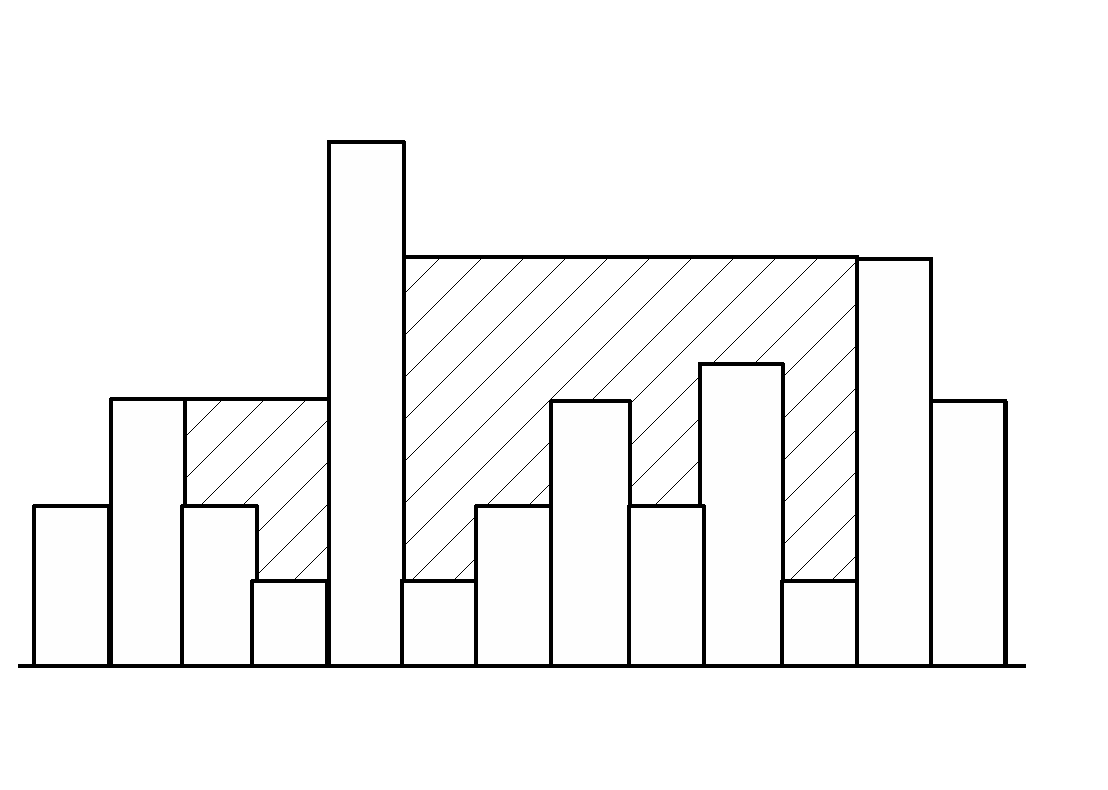
\includegraphics[scale=0.3]{scan/rain-fill/img/rain-fill.eps}
 \caption{灰色的区域表示积水。}
 \label{fig:rain-fill}
\end{figure}
例如,等高地图数据为$\{0,1,0,2,1,0,1,3,2,1,2,1\}$,则积水数量为6。
\item 解释在看起来“最坏”的情况下,为何KMP算法的性能仍然为线性?
\item 使用逆序的$P_p$以避免线性时间的添加操作,改进实现纯函数式的KMP算法。
\item 在文本“anal”中搜索字符串“ananym”,试推导树$left(right(right(right(T))))$的状态。
\end{itemize}
\end{Exercise}

\section{解的搜索}

计算机程序可以用于解答某些趣题。在人工智能的早期阶段,人们发展出了搜索解的许多方法。和序列搜索、字符串匹配不同,问题的解并不一定直接存在于一个候选答案集中。往往需要一边构造解,一边进行尝试。某些问题可解,同时也存在大量无解的问题。即使是有解的问题,也通常存在多个解。例如,一个迷宫可能存在多种走出的路线。人们往往需要求出某种意义下的最优解。

\subsection{深度优先搜索(DFS)和广度优先搜索(BFS)}
\index{DFS} \index{Deep-first search}
DFS和BFS分别代表深度优先搜索和广度优先搜索。它们通常作为图搜索算法加以介绍。图是一个很大的题目,超出了本书讲述的基本算法的范围。本节中,我们主要介绍如何使用DFS和BFS解决某些趣题,而不会正式介绍图的概念。

\subsubsection{迷宫}
\index{Maze problem}
迷宫的历史悠久,广受欢迎、是老少皆宜的一类趣题。图\ref{fig:maze}给出了一个迷宫的例子。在某些公园,甚至还建有真正的迷宫供人游玩。在1990年代末,机器老鼠走迷宫的竞赛一度在世界上流行。

\begin{figure}[htbp]
 \centering
 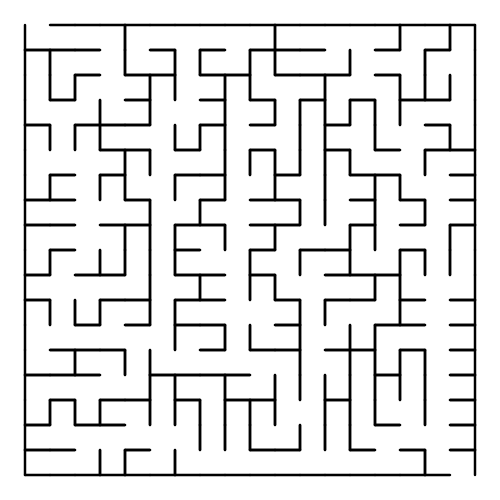
\includegraphics[scale=0.3]{img/maze.eps}
 \caption{一个迷宫的例子}
 \label{fig:maze}
\end{figure}

迷宫有很多解法。本节将介绍一种有效的、但并非最好的方法。有很多针对迷宫解法的古老谚语,但是它们并非全都正确。

例如,有一个说法,当遇到分叉道路时,总向右转。如图\ref{fig:maze-loop}所示,这一招并不灵。明显可以先沿着上方的水平线前进,然后向右转,接着一直前进,经过T字路口就可到达终点。但如果遇到岔路就向右转,就会绕着中心的大方块不断转圈。

\begin{figure}[htbp]
 \centering
 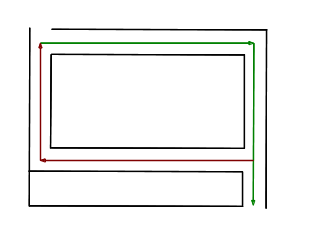
\includegraphics[scale=0.6]{img/maze-loop.eps}
 \caption{如果一直右转,就会陷入循环。}
 \label{fig:maze-loop}
\end{figure}

这个例子说明,当存在多个选项时,做出的决策会直接影响到最终的解。就像我们小时候读的童话故事,我们可以携带一块面包进入迷宫。当遇到岔路时,我们任选一条道路,然后留下一小块面包屑记录下这次尝试。如果我们遇到了死胡同,就沿着留下的面包屑向回走到上次做出选择的地方,然后换一条路。

任何时候,如果我们发现地上已经有面包屑了,就说明我们进入了循环,必须向回退然后重新尝试。不断重复这样的“尝试——检查”,我们或者最终找到走出迷宫的路,或者得知这个迷宫无解,此时我们最终回退到了迷宫的起点。

一种简单的描述迷宫的方法,是使用$m \times n$的矩阵,每个元素的值为0或1,表示这一位置是否有路。图\ref{fig:maze-loop}所示的迷宫可以用下面的矩阵定义。

\[
\begin{matrix}
0 & 0 & 0 & 0 & 0 & 0 \\
0 & 1 & 1 & 1 & 1 & 0 \\
0 & 1 & 1 & 1 & 1 & 0 \\
0 & 1 & 1 & 1 & 1 & 0 \\
0 & 1 & 1 & 1 & 1 & 0 \\
0 & 0 & 0 & 0 & 0 & 0 \\
1 & 1 & 1 & 1 & 1 & 0
\end{matrix}
\]

给定起点$s=(i, j)$和终点$e=(p, q)$,我们要找出所有的解,也就是从$s$到$e$的全部路径。

显然存在一个递归的穷举搜索方法。为了找到所有从$s$到$e$的路径,我们可以检查和$s$连通的所有相邻点,对于每个点$k$,我们递归找出从$k$到$e$的所有路径。这一方法可以描述如下。

\begin{itemize}
\item 边界情况,如果起点$s$和终点$e$相同,搜索结束;
\item 否则,对所有和$s$连通的相邻点$k$,递归找出从$k$到$e$的全部路径;如果可以通过$k$到达$e$,将通路$s$-$k$连接到每个从$k$到$e$的路径前面。
\end{itemize}

但是,我们必须留下一下“面包屑”以避免重复尝试。否则,在递归的情况下,我们从$s$找到了一个连通点$k$,然后我们继续寻找从$k$到$e$的路径。由于$s$同样和$k$连通,所以在接下来的递归中,我们将再次寻找从$s$到$e$的通路。这样就陷入了此前描述过的无穷循环中。

我们的解法是初始化一个空列表,用以记录我们走过的所有位置。对于每个连通的点,我们查找这一列表,看是否已经走过。我们跳过所有已走过的位置,而只尝试新的路径。对应的算法定义如下。

\be
solveMaze(m, s, e) = solve(s, \{ \phi \})
\label{eq:solve-maze-reversed}
\ee

其中$m$是定义迷宫的矩阵,$s$是起点,$e$是中点。函数$solve$定义在$solveMaze$的环境中,因此可以直接访问迷宫和中点。它的具体定义如下\footnote{函数$concat$可以将一组列表连接起来,例如:$concat(\{\{a, b, c\}, \{x, y, z\}\}) = \{a, b, c, x, y, z\}$。具体可以参见附录A。}。

\be
solve(s, P) = \left \{
  \begin{array}
  {r@{\quad:\quad}l}
  \{ \{ s\} \cup p | p \in P \} & s = e \\
  \begin{array}{rl}
  concat(\{ & solve(s', \{ \{ s\} \cup p | p \in P \}) | \\
            & s' \in adj(s), \lnot visited(s')\})
  \end{array} & otherwise
  \end{array}
\right.
\ee

这里$P$相当于一个累积器(accumulator)。每个连通的点都被记录在和当前位置连通的路径中。但是它们的顺序是逆序的,新走到的点被放在所有列表的头部,而起点被放在最后。这是因为列表的尾部添加操作是线性时间的($O(n)$,其中$n$是列表中保存的元素个数),而在头部添加的操作是常数时间的。为了输出正常的路径顺序,我们可以将式(\ref{eq:solve-maze-reversed})所有的解都反转\footnote{$reverse$的具体定义可以参见附录A。}。

\be
solveMaze(m, s, e) = map(reverse, solve(s, \{ \phi \}))
\ee

接下来需要定义函数$adj(p)$和$visited(p)$,前者找出所有和点$p$相连通的店,后者检查点$p$是否以前已经尝试走过。如果矩阵中水平方向,或者垂直方向上的相邻元素,值都为0,我们定义这两个点连通。

\be
\begin{array}{ll}
adj((x, y)) = \{ (x', y') | & (x', y') \in \{ (x-1, y), (x+1, y), (x, y-1), (x, y+1)\}, \\
 & 1 \leq x' \leq M, 1 \leq y' \leq N, m_{x' y'} = 0\} \\
\end{array}
\ee

其中$M$和$N$分别是迷宫的宽和高。

函数$visited(p)$检查点$p$是否已记录在列表$P$中的某一路径上。

\be
visited(p) = \exists path \in P, p \in path
\ee

下面的Haskell例子程序实现了这一走迷宫算法。

\lstset{language=Haskell}
\begin{lstlisting}
solveMaze m from to = map reverse $ solve from [[]] where
    solve p paths | p == to = map (p:) paths
                  | otherwise = concat [solve p' (map (p:) paths) |
                                        p' <- adjacent p,
                                        not $ visited p' paths]
    adjacent (x, y) = [(x', y') |
                    (x', y') <- [(x-1, y), (x+1, y), (x, y-1), (x, y+1)],
                    inRange (bounds m) (x', y'),
                    m ! (x', y') == 0]
    visited p paths = any (p `elem`) paths
\end{lstlisting} %$

对于下面例子中给出的迷宫,这一程序可以给出全部的解。

\lstset{language=Haskell}
\begin{lstlisting}
mz = [[0, 0, 1, 0, 1, 1],
      [1, 0, 1, 0, 1, 1],
      [1, 0, 0, 0, 0, 0],
      [1, 1, 0, 1, 1, 1],
      [0, 0, 0, 0, 0, 0],
      [0, 0, 0, 1, 1, 0]]

maze  = listArray ((1,1), (6, 6)) . concat

solveMaze (maze mz) (1,1) (6, 6)
\end{lstlisting}

我们此前提到,这事一种“穷举搜索”的解法,它递归地搜索所有连通的点作为候选。在实际的迷宫竞赛中,例如机器老鼠走迷宫竞赛,找到一条路径就足够了。我们可以调整解法,它和本节开始时描述的方法类似,机器老鼠总是选择第一个连通点,而跳过其他选择直到无法前进。我们需要某种数据结构保存“面包屑”,记录此前做出的决策。由于我们总是在最新的决策基础上搜索通路,因此是后进先出的顺序。我们可以使用一个栈来实现。

在开始的时候,只有起点$s$保存在栈中。我们将其弹出,找出和$s$相连通的点,例如$a$和$b$。然后我们将两条可能的路径$\{a, s\}$和$\{b, s\}$推入栈中。接下来,我们将路径$\{a, s\}$弹出,然后检查和点$a$相连通的点。然后所有经过3步可到达的路径被推回栈。我们重复这一过程。任何时候,栈中的每个元素都代表一条逆序的路径,它从起点开始,通向可到达的最远位置。如图\ref{fig:dfs-stack}所示。

\begin{figure}[htbp]
 \centering
 \includegraphics[scale=0.5]{img/dfs-stack.ps}
 \caption{栈初始时包含一个只有一个元素的列表。这一元素为起点$s$。$s$和点$a$、$b$连通。路径$\{a, s\}$和$\{b, s\}$被推回栈。在某一步,以$p$结束的路径被弹出。$p$和点$i$、$j$和$k$连通。这3个点被扩展为不同的选项,并推回到栈中。除非所有的候选路径都失败,否则不会尝试以$q$结尾的候选路径。}
 \label{fig:dfs-stack}
\end{figure}

栈可以用一个列表来实现。最新的选项可以从表头获得,新的候选路径也被添加到表头。可以通过这样的路径列表解决迷宫问题。

\be
solveMaze'(m, s, e) = reverse(solve'(\{\{s\}\}))
\ee

由于我们搜索第一个,而不是全部的解,这里我们没有使用$map$函数。当栈为空时,表示我们已经尝试了所有的可能,但仍然没有找到通路。因此迷宫无解;否则,我们弹出栈顶的候选路径,将其扩展到所有未曾走过的连通点,然后再推回栈。我们用$S$表示栈,若栈不为空,则栈顶的元素记为$s_1$,弹出栈顶元素后的新栈表示为$S'$。$s_1$为一个点的列表,代表路径$P$。记这条路径中的第一个点位$p_1$,其余的点位$P'$。这一解法可以定义如下。

\be
solve'(S) = \left \{
  \begin{array}
  {r@{\quad:\quad}l}
  \phi & S = \phi \\
  s_1 & s_1 = e \\
  solve'(S') & C = \{ c | c \in adj(p_1), c \not\in P' \} = \phi \\
  solve'(\{ \{p\}\cup P | p \in C\} \cup S) & otherwise, C \neq \phi
  \end{array}
\right.
\ee

其中$adj$的定义和前面相同。下面的Haskell例子程序实现了这一迷宫算法\footnote{$ajacent$函数的定义完全相同,在此略过。}。

\lstset{language=Haskell}
\begin{lstlisting}
dfsSolve m from to = reverse $ solve [[from]] where
    solve [] = []
    solve (c@(p:path):cs)
        | p == to = c -- stop at the first solution
        | otherwise = let os = filter (`notElem` path) (adjacent p) in
                          if os == []
                          then solve cs
                          else solve ((map (:c) os) ++ cs)
\end{lstlisting} %$

可以很容易地修改这一算法,从而找到全部的解。在第二行找到一个解后,我们不立即返回,我们将其记录下来,然后继续尝试栈中记录的其他候选路径,直到栈变为空。我们将其作为练习留给读者。

也可以用命令式的方法实现这一思路。我们使用一个栈保存从起点开始的全部可能路径。每次迭代,首先弹出栈顶保存的路径,如果这一路径到达了终点,则找到了迷宫的一个解;否则,我们将尚未尝试过的所有连通点添加到路径上作为新的候选路径,并推回栈。重复这一过程知道栈中的所有候选路径都检查完毕。

我们使用同样的符号$S$表示栈。但在命令式的环境中,路径使用数组来表示,这样效率更高。为此,起点保存在数组的第一个元素中,二最远到达的点保存为最右侧的元素。我们用$P_n$来表示路径$P$中的最后一个元素\textproc{Last}($P$)。命令式的算法定义如下。

\begin{algorithmic}[1]
\Function{Solve-Maze}{$m, s, e$}
  \State $S \gets \phi$
  \State \Call{Push}{$S, \{ s \}$}
  \State $L \gets \phi$ \Comment{结果列表}
  \While{$S \neq \phi$}
    \State $P \gets$ \Call{Pop}{$S$}
    \If{$e = p_n$}
      \State \Call{Add}{$L, P$}
    \Else
      \For{$\forall p \in $ \Call{Adjacent}{$m, p_n$}}
        \If{$p \notin P$}
          \State \Call{Push}{$S, P \cup \{ p \}$}
        \EndIf
      \EndFor
    \EndIf
  \EndWhile
  \State \Return $L$
\EndFunction
\end{algorithmic}

下面的Python例子程序实现了这一迷宫算法。

\lstset{language=Python}
\begin{lstlisting}
def solve(m, src, dst):
    stack = [[src]]
    s = []
    while stack != []:
        path = stack.pop()
        if path[-1] == dst:
            s.append(path)
        else:
            for p in adjacent(m, path[-1]):
                if not p in path:
                    stack.append(path + [p])
    return s

def adjacent(m, p):
    (x, y) = p
    ds = [(0, 1), (0, -1), (1, 0), (-1, 0)]
    ps = []
    for (dx, dy) in ds:
        x1 = x + dx
        y1 = y + dy
        if 0 <= x1 and x1 < len(m[0]) and
           0 <= y1 and y1 < len(m) and m[y][x] == 0:
            ps.append((x1, y1))
    return ps
\end{lstlisting}

同样的例子迷宫可以用这一程序解决如下。

\lstset{language=Python}
\begin{lstlisting}
mz = [[0, 0, 1, 0, 1, 1],
      [1, 0, 1, 0, 1, 1],
      [1, 0, 0, 0, 0, 0],
      [1, 1, 0, 1, 1, 1],
      [0, 0, 0, 0, 0, 0],
      [0, 0, 0, 1, 1, 0]]

solve(mz, (0, 0), (5,5))
\end{lstlisting}

看上去在最坏的情况下,每步都有上下左右4个选项,每个选项都被推入栈,并且最终在回溯时都被检查了。算法的复杂度看似是$O(4^n)$。实际上消耗的时间并不会这样大,这是因为我们过滤掉了已经走过的位置。在最坏情况下,所有可以到达的点都恰好被访问过一次。因此时间复杂度为$O(n)$,其中$n$是互相连通的点的数量。由于使用了一个栈来保存候选路径,空间复杂度为$O(n^2)$。

\subsubsection{八皇后问题}
\index{8 queens puzzle}

八皇后问题是一个很著名的趣题。虽然国际象棋有着悠久的历史,八皇后趣题却最早在1848年由Max Bezzel提出\cite{wiki-8-queens}。皇后是国际象棋中一种威力巨大的棋子。她可以攻击在同一行、列和斜线上的任意距离的其他棋子。这道趣题是要求找到一种方法,可以在棋盘上同时摆下八个皇后,而她们之间不会互相攻击。图\ref{fig:8-queens-puzzle} (a)描述了皇后可以攻击到的范围。图\ref{fig:8-queens-puzzle} (b)给出了八皇后问题的某一种解。

\begin{figure}[htbp]
 \centering
 \subfloat[国际象棋中的皇后。]{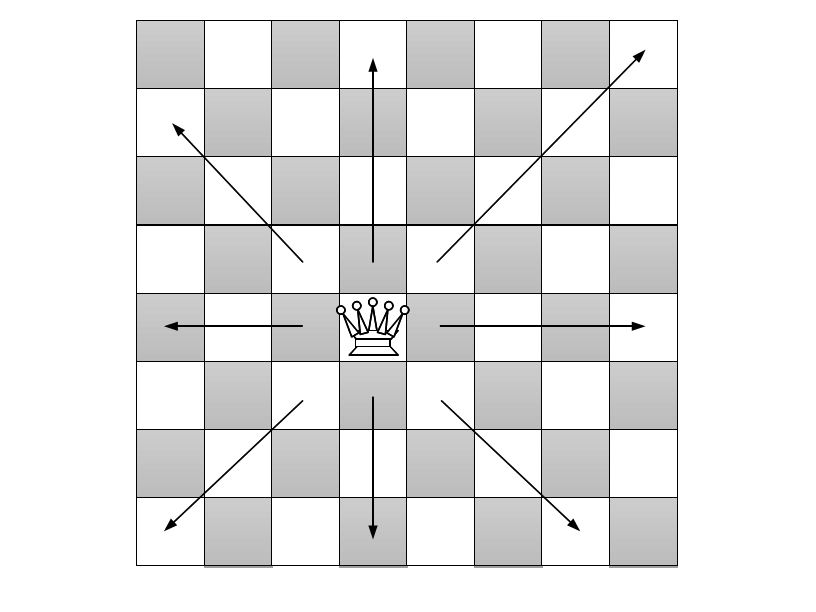
\includegraphics[scale=1]{img/queen.eps}}
 \subfloat[某一种解。]{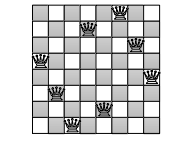
\includegraphics[scale=1]{img/queens-example.eps}}
 \caption{八皇后问题。}
 \label{fig:8-queens-puzzle}
\end{figure}

显然,可以用暴力方法穷举解决八皇后问题,在国际象棋棋盘的64个格子中,放入8个皇后,这需要在$P^8_{64}$个可能的排列中检查。这个数字大约为$4 \times 10^{10}$。显然我们可以改进这一方法,考虑任一行中不能包含2个及以上的皇后,并且任何一个皇后都必须放在第1列到第8列中的某一列上,所以一个解的布局必然是$\{1,2,3,4,5,6,7,8\}$的某种排列。例如布局$\{6,2,7,1,3,5,8,4\}$表示,第一个皇后摆放在第1行、第6列上;第二个皇后摆在第2行、第2列上……最后一个皇后摆在第8行、第4列上。通过这一方法,我们只需要检查$8! = 40320$种可能的布局。

我们可以找到更好的解法。和迷宫问题类似,我们可以从第一行开始,逐一摆放皇后。对于第一个皇后,存在8种可能的摆法,她可以被放置在八列中的某一列上。接下来摆放第二个皇后,我们检查8个可能的列。由于可能被第一个皇后攻击,因此某些列不能再摆放了。我们重复这一过程,对于第$i$个皇后,我们检查第$i$行中的8个位置,找到不被任何前$i-1$个皇后攻击的位置。如果所有8个位置都不能摆放,即这一行的8个位置都会被此前摆放过的某个皇后攻击,我们就必须向迷宫问题中一样进行回溯。当所有8个皇后都成功放入棋盘后,我们就找到了一个可行的解。为了找到所有可能解,我们需要记录下这一布局,然后继续检查其他可能的列,并进行必要的回溯。当第一行的8列都尝试完毕后,这一过程结束。下面的函数启动八皇后问题解的查找过程。

\be
solve(\{\phi\}, \phi)
\ee

和迷宫问题类似,我们使用一个栈$S$来记录可能的尝试。一开始栈中只有一个空元素。我们使用一个列表$L$来记录所有可行的解。记栈顶的元素为$s_1$。它是某种尚未完成的布局,也就是1到8中部分元素的排列。将栈顶元素$s_1$弹出后,剩下的部分记为$S'$。函数$solve$的具体定义如下。

\be
solve(S, L) = \left \{
  \begin{array}
  {r@{\quad:\quad}l}
  L & S = \phi \\
  solve(S', \{s_1\} \cup L) & |s_1| = 8 \\
  solve(\left \{
      \begin{array}{rl}
        \{i\} \cup s_1 | & i \in [1,8], \\
                         & i \notin s_1, \\
                         & safe(i, s_1)
      \end{array}
      \right \} \cup S', L) & otherwise
  \end{array}
\right.
\ee

若栈为空,表明所有可能都已经尝试完毕,我们已无法继续回溯了。列表$L$已记录下了所有找到的解,我们将其作为结果返回;否额,若栈顶元素所代表的布局长度为8,表明我们找到了一种可行的解。我们将其记录到$L$中,然后继续寻找其它的解;如果这一布局的长度小于8,表明我们需要继续摆放剩余的皇后。我们从第1到第8列中,找出尚未被占的列(通过$i \notin s_1$条件),同时它不能被斜线上的其他皇后攻击(通过$safe$条件)。可行的布局被推入栈中用于此后的搜索。

函数$safe(x, C)$检查在位置$x$上的皇后是否会被$C$中的任意皇后,从斜线方向攻击。有两种可能的情况,分别是$45^{\circ}$度和$135^{\circ}$度方向。由于这一皇后所在的行为$y = 1 + |C|$,其中$|C|$是中间布局$C$的长度。函数$safe$可定义如下。

\be
safe(x, C) = \forall (c, r) \in zip(reverse(C), \{1, 2, ...\}), |x - c| \neq |y - r|
\ee

其中$zip$将两个列表中的每个元素都结合成一对,组成一个新的列表。因此,若$C = \{ c_{i-1}, c_{i-2}, ..., c_2, c_1\}$代表前$i-1$个皇后分别所在的列,上述函数将检查每个皇后的行列位置$\{(c_1, 1), (c_2, 2), ..., (c_{i-1}, i-1)\}$是否会和位置$(x, y)$构成对角线。

下面的Haskell例子程序实现了这一八皇后问题的解。

\lstset{language=Haskell}
\begin{lstlisting}
solve = dfsSolve [[]] [] where
    dfsSolve [] s = s
    dfsSolve (c:cs) s
             | length c == 8 = dfsSolve cs (c:s)
             | otherwise = dfsSolve ([(x:c) | x <- [1..8] \\ c,
                               not $ attack x c] ++ cs) s
    attack x cs = let y = 1 + length cs in
                  any (\(c, r) -> abs(x - c) == abs(y - r)) $
                      zip (reverse cs) [1..]
\end{lstlisting}

观察到这一算法是尾递归的,它可以很容易地用命令式的方式实现。我们使用数组而非列表来表示皇后的布局。及栈为$S$,中间布局为$A$,命令式算法可以描述如下。

\begin{algorithmic}[1]
\Function{Solve-Queens}{}
  \State $S \gets \{\phi\}$
  \State $L \gets \phi$ \Comment{保存所有解的列表}
  \While{$S \neq \phi$}
    \State $A \gets$ \Call{Pop}{$S$} \Comment{$A$是某一中间布局}
    \If{$|A|=8$}
      \State \Call{Add}{$L, A$}
    \Else
      \For{$i \gets 1$ to $8$}
        \If{\Call{Valid}{$i, A$}}
          \State \Call{Push}{$S, A \cup \{i\}$}
        \EndIf
      \EndFor
    \EndIf
  \EndWhile
  \State \Return $L$
\EndFunction
\end{algorithmic}

栈中一开始放入一个空布局。然后不断取出栈顶元素,如果还有皇后尚未摆放完毕,我们就依次检查下一行中的所有8个位置。如果该位置是安全的,也就是说它不被此前的任意皇后攻击,就将此位置添加到布局中,并推回堆栈。和函数式方法不同,由于使用数组,我们无需再将解的布局反转。

函数\textproc{Valid}检查中间布局$A$中的下一行的$x$列位置摆放皇后是否安全。它去掉已经被占的列,然后计算对角线上是否有别的皇后。

\begin{algorithmic}[1]
\Function{Valid}{$x, A$}
  \State $y \gets 1 + |A|$
  \For{$i \gets 1$ to $|A|$}
    \If{$x = i \lor |y-i| = |x - A[i]|$}
      \State \Return False
    \EndIf
  \EndFor
  \State \Return True
\EndFunction
\end{algorithmic}

下面的Python例子程序实现了这一命令式八皇后解法。

\lstset{language=Python}
\begin{lstlisting}
def solve():
    stack = [[]]
    s = []
    while stack != []:
        a = stack.pop()
        if len(a) == 8:
            s.append(a)
        else:
            for i in range(1, 9):
                if valid(i, a):
                    stack.append(a+[i])
    return s

def valid(x, a):
    y = len(a) + 1
    for i in range(1, y):
        if x == a[i-1] or abs(y - i) == abs(x - a[i-1]):
            return False
    return True
\end{lstlisting}

虽然摆放每个皇后时有8列可供选择,但是并非所有列都可行。只有此前没有被占的列才会被尝试。算法只检查15720种情况,这要远远小于$8^8 = 16777216$种可能\cite{wiki-8-queens}。

可以很容易将这一算法加以扩展,用以解决$n$皇后问题,其中$N \geq 4$。但是随着$n$的增大,所用的时间急速增加。这一回溯算法仅仅比枚举1到8的全排列稍快(枚举全排列的时间是$o(n!)$)。此外,还存在另一种小改进,由于国际象棋棋盘是正方形的,它水平方向和垂直方向都对称。因此得到一个解后,通过旋转和翻转,可以得到其他对称的解。我们将这一改进留给读者作为练习。

\subsubsection{跳棋趣题}
\index{Peg puzzle}

我曾经收到过一道关于跳跃的青蛙的趣题。据说这是中国二年级小学生的家庭作业。如图\ref{fig:leapfrog}所示,在7块排成一排的石头上有6只青蛙。如果前方的石头是空的,青蛙可以跳到石头上;青蛙还可以越过一只青蛙,调到前方的空石头上。左侧的青蛙只能向右侧前进,而右侧的青蛙只能向左侧前进。图\ref{fig:pegrules}描述了青蛙跳跃的规则。

\begin{figure}[htbp]
 \centering
 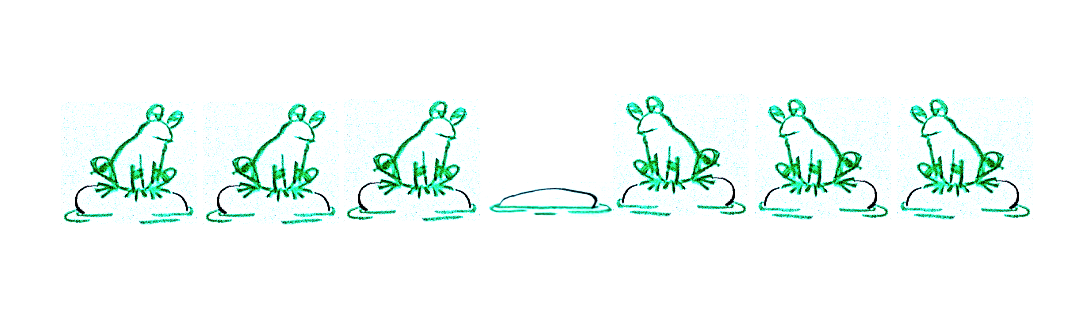
\includegraphics[scale=0.4]{img/leapfrogs.eps}
 \caption{跳跃的青蛙趣题。}
 \label{fig:leapfrog}
\end{figure}

这道题目要求按照规则安排青蛙移动或者跳跃,使得左右的3只青蛙位置互换。如果我们标记左侧的青蛙为A,右侧的为B,没有青蛙的石头为O,这道题目就是要求找到要给解使得从AAAOBBB转换到BBBOAAA。

\begin{figure}[htbp]
 \centering
 \subfloat[跳到相邻的石头上。]{
\includegraphics[scale=0.3]{img/leapfrog1.eps}} \hspace{0.02\textwidth}
 \subfloat[向右侧越过一只青蛙。]{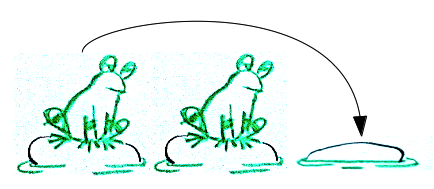
\includegraphics[scale=0.3]{img/leapfrog2.eps}} \hspace{0.02\textwidth}
 \subfloat[向左侧越过一只青蛙。]{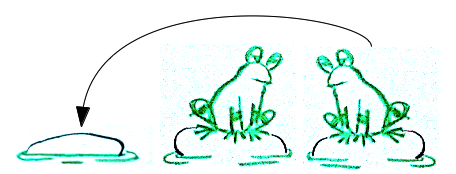
\includegraphics[scale=0.3]{img/leapfrog3.eps}}
 \caption{移动规则。}
 \label{fig:pegrules}
\end{figure}

这道趣题是跳棋类趣题的一个特殊形式。跳棋的个数并不一定限制为6,它可以是8或者更大的偶数。图\ref{fig:pegpuzzles}给出了一些这类问题的变化形式。

\begin{figure}[htbp]
 \centering
 \subfloat[单人跳棋(Solitaire)]{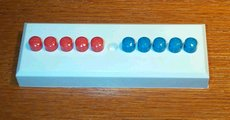
\includegraphics[scale=0.5]{img/solitaire.eps}} \hspace{0.02\textwidth}
 \subfloat[Hop over]{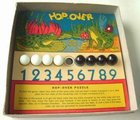
\includegraphics[scale=0.7]{img/hop-over.eps}} \hspace{0.02\textwidth}
 \subfloat[Draught board]{
\includegraphics[scale=0.3]{img/draught-board.eps}}
 \caption{跳棋趣题的变化形式,来自http://home.comcast.net/~stegmann/jumping.htm}
 \label{fig:pegpuzzles}
\end{figure}

我们可以通过编程的方法解决这类趣题。思路和八皇后问题类似。记从左向右的石头位置为1, 2, ..., 7。理想情况下,有4种可能的移动。例如游戏开始的时候,第3块石头上的青蛙可以移动到空石头上;对称地,第5块石头上的青蛙也可以向左移动一步;另外,第2块石头上的青蛙可以向右越过一只青蛙,跳到空石头上,同样,第6块石头上的青蛙,也可以向左越过一只青蛙。

每走一步,我们可以记录下青蛙们的状态,然后尝试4种方案中的一种。当然并非任何时候,4种方案都可行。如果我们走不下去了,就回溯并尝试其他方案。

由于我们限制左侧的青蛙只能向右,右侧的青蛙只能向左,因此这些移动都是不可逆的。和迷宫游戏不同,这里不可能存在重复的情况。但是,我们仍需记录移动的步骤,以便最后的输出。

为了强调这些条件,我们分别用-1、0、和1代表A、O、和B。一个状态就是一列元素,每个元素是这3个值中的一种。起始状态为$\{-1, -1, -1, 0, 1, 1, 1\}$。$L[i]$表示第$i$个元素,它的值表明第$i$个石头是否为空,或者存在一只左侧移动来的青蛙,或者存在一只右侧移动来的青蛙。记空石头的位置为$p$。4种可能的移动方案可以描述如下。

\begin{itemize}
\item 向左跳跃(Leap left):$p < 6$,且$L[p+2] > 0$,交换$L[p] \leftrightarrow L[p+2]$;
\item 向左移动(Hop left):$p < 7$,且$L[p+1] > 0$,交换$L[p] \leftrightarrow L[p+1]$;
\item 向右跳跃(Leap right):$p > 2$,且$L[p-2] < 0$,交换$L[p-2] \leftrightarrow L[p]$;
\item 向右移动(Hop right):$p > 1$,且$L[p-1] < 0$,交换$L[p-1] \leftrightarrow L[p]$。
\end{itemize}

为此,我们定义4个函数$leap_l(L)$、$hop_l(L)$、$leap_r(L)$、和$hop_r(L)$。若$L$不满足移动的条件,这些函数将返回同样的$L$,否则,它们返回变化后的状态$L'$。

我们可以使用一个栈$S$来保存已做过的尝试。开始的时候,栈中包含一个列表,列表中只有一个元素,就是开始状态。我们将找到的解保存在列表$M$中,$M$起始为空。

\be
solve(\{\{-1, -1, -1, 0, 1, 1, 1\}\}, \phi)
\ee

只要栈不为空,我们就取出栈顶元素。如果最后的状态等于$\{1, 1, 1, 0, -1, -1, -1\}$,说明找到了一个解。我们将直到这一状态的一系列移动方案添加到$M$中;否则,我们在最后的状态上尝试4种可能的移动,并将可行的移动方法推回栈以便将来继续搜索。记堆栈为$S$,栈顶的元素为为$s_1$,$s_1$中记录的最后的状态为$L$。算法可以定义如下。

\be
solve(S, M) = \left \{
  \begin{array}
  {r@{\quad:\quad}l}
  M & S = \phi \\
  solve(S', \{reverse(s_1)\} \cup M) & L = \{1, 1, 1, 0, -1, -1, -1\} \\
  solve(P \cup S', M) & otherwise
  \end{array}
\right.
\ee

其中$P$是在最后的状态$L$之上可能的移动方法:
\[
P = \{ L'  | L' \in \{leap_l(L), hop_l(L), leap_r(L), hop_r(L)\}, L \neq L'\}
\]

起始状态被保存为最后一个元素,而最后的状态是第一个元素。因此我们需要将其反转,保存在解的列表中。

下面的Haskell例子程序,实现了跳跃青蛙问题的解。

\lstset{language=Haskell}
\begin{lstlisting}
solve = dfsSolve [[[-1, -1, -1, 0, 1, 1, 1]]] [] where
    dfsSolve [] s = s
    dfsSolve (c:cs) s
             | head c == [1, 1, 1, 0, -1, -1, -1] = dfsSolve cs (reverse c:s)
             | otherwise = dfsSolve ((map (:c) $ moves $ head c) ++ cs) s

moves s = filter (/=s) [leapLeft s, hopLeft s, leapRight s, hopRight s] where
    leapLeft [] = []
    leapLeft (0:y:1:ys) = 1:y:0:ys
    leapLeft (y:ys) = y:leapLeft ys
    hopLeft [] = []
    hopLeft (0:1:ys) = 1:0:ys
    hopLeft (y:ys) = y:hopLeft ys
    leapRight [] = []
    leapRight (-1:y:0:ys) = 0:y:(-1):ys
    leapRight (y:ys) = y:leapRight ys
    hopRight [] = []
    hopRight (-1:0:ys) = 0:(-1):ys
    hopRight (y:ys) = y:hopRight ys
\end{lstlisting}

运行这一程序可以找出2个对称的解,每个都需要15步。下表列出了其中的一个解。

\begin{tabular}{|c||c|c|c|c|c|c|c|}
\hline
step & -1 & -1 & -1 & 0 & 1 & 1 & 1 \\
\hline
1 & -1 & -1 & 0 & -1 & 1 & 1 & 1 \\
2 & -1 & -1 & 1 & -1 & 0 & 1 & 1 \\
3 & -1 & -1 & 1 & -1 & 1 & 0 & 1 \\
4 & -1 & -1 & 1 & 0 & 1 & -1 & 1 \\
5 & -1 & 0 & 1 & -1 & 1 & -1 & 1 \\
6 & 0 & -1 & 1 & -1 & 1 & -1 & 1 \\
7 & 1 & -1 & 0 & -1 & 1 & -1 & 1 \\
8 & 1 & -1 & 1 & -1 & 0 & -1 & 1 \\
9 & 1 & -1 & 1 & -1 & 1 & -1 & 0 \\
10 & 1 & -1 & 1 & -1 & 1 & 0 & -1 \\
11 & 1 & -1 & 1 & 0 & 1 & -1 & -1 \\
12 & 1 & 0 & 1 & -1 & 1 & -1 & -1 \\
13 & 1 & 1 & 0 & -1 & 1 & -1 & -1 \\
14 & 1 & 1 & 1 & -1 & 0 & -1 & -1 \\
15 & 1 & 1 & 1 & 0 & -1 & -1 & -1 \\
\hline
\end{tabular}

观察上述算法,它是尾递归的,因此可以较容易地用命令式方式实现。我们将算法扩展为解决每侧有$n$只青蛙的题目。记起始状态$s$为\{-1, -1, ..., -1, 0, 1, 1, ..., 1\},左右翻转后的终止状态为$e$。

\begin{algorithmic}[1]
\Function{Solve}{$s, e$}
  \State $S \gets \{\{s\}\}$
  \State $M \gets \phi$
  \While{$S \neq \phi$}
    \State $s_1 \gets$ \Call{Pop}{$S$}
    \If{$s_1[1] = e$}
      \State \textproc{Add}($M$, \Call{Reverse}{$s_1$})
    \Else
      \For{$\forall m \in$ \Call{Moves}{$s_1[1]$}}
        \State \textproc{Push}($S$, $\{m\} \cup s_1$)
      \EndFor
    \EndIf
  \EndWhile
  \State \Return $M$
\EndFunction
\end{algorithmic}

可能的移动方法可以被实现为\textproc{Moves}过程。它可以处理任意只青蛙的情况。下面的Python程序实现了这一解法。

\lstset{language=Python}
\begin{lstlisting}
def solve(start, end):
    stack = [[start]]
    s = []
    while stack != []:
        c = stack.pop()
        if c[0] == end:
            s.append(reversed(c))
        else:
            for m in moves(c[0]):
                stack.append([m]+c)
    return s

def moves(s):
    ms = []
    n = len(s)
    p = s.index(0)
    if p < n - 2 and s[p+2] > 0:
        ms.append(swap(s, p, p+2))
    if p < n - 1 and s[p+1] > 0:
        ms.append(swap(s, p, p+1))
    if p > 1 and s[p-2] < 0:
        ms.append(swap(s, p, p-2))
    if p > 0 and s[p-1] < 0:
        ms.append(swap(s, p, p-1))
    return ms

def swap(s, i, j):
    a = s[:]
    (a[i], a[j]) = (a[j], a[i])
    return a
\end{lstlisting}

对于每侧有3只青蛙的情况,我们知道共需要15步才能让它们左右互换。通过上述算法,我们可以得到解法的步数和每侧青蛙数目的一个关系,如下表:

\begin{tabular}{c|c|c|c|c|c|c}
每侧青蛙的数目 & 1 & 2 & 3  & 4  & 5 & ... \\
\hline
解法的步数 & 3 & 8 & 15 & 24 & 35 & ...
\end{tabular}

表中列出的解法的步数恰好是完全平方数减一。因此我们猜测,解法的步数和每侧青蛙的数目$n$的关系为$(n+1)^2 - 1$。实际上,我们可以证明这一点。

比较最终的状态和最初的状态,每只青蛙都向相对的一侧移动了$n+1$块石头。因此$2n$只青蛙,总共移动了$2n(n+1)$块石头。另一个重要的事实是,左侧的每只青蛙,必然和右侧的所有青蛙相遇一次。一旦相遇,必然发生一次跳跃。由于一共有$n^2$次相遇,因此共导致了所有青蛙前进了$2n^2$块石头。剩下的移动不是跳跃,而是跳到相邻的石头上,总共有$2n(n+1) - 2n^2 = 2n$次。将$n^2$次跳跃,和$2n$次调到相邻石头上相加。得到最终解的步数为:$n^2 + 2n = (n+1)^2 -1$。

\subsubsection{深度优先搜索的小结}

观察上述3个趣题,虽然它们各不相同,但是它们的解法却有着类似的结构。它们都有着某种启示状态。迷宫问题从入口开始;八皇后问题从空棋盘开始;跳跃青蛙问题从AAAOBBB的状态开始。解的过程是一种搜索,每次尝试,都有若干种可能的选项。迷宫问题中,没走一步都有上下左右四个方向可供选择;八皇后问题中,每次摆放都由8列可供选择;跳跃青蛙趣题中,每次尝试都有4种不同的跳跃方式可供选择。虽然每次选择,我们都不知能继续走多远。但我们始终清楚地知道最终状态是什么。在迷宫问题中,最终状态是出口;八皇后问题中,最终状态是8个皇后都摆放在棋盘上;跳跃青蛙趣题中,最终状态是所有所有青蛙的位置互换。

我们使用相同的策略来解决这些问题。我们不断选择可能的选项尝试,记录已经达到的状态,如果无法继续就进行回溯并尝试其他选项。通过这样的方法,我们或者可以找到解,或者穷尽所有可能而发现问题无解。

当然,这类解法还存在一些变化,当找到一个解后,我们可以停下结束,或者继续寻找所有可能的解。

如果我们以起始状态为根,画出一棵树,每个树枝代表一个不同的选择。我们的搜索过程,是一个不断深入的过程。只要能够继续,我们就不考虑同一深度上的其他选项。知道失败后回溯到树的上一层。图\ref{fig:dfs-tree}描述了我们在状态树种的搜索顺序。箭头方向表明了我们如何先向下,在向上回溯的过程。节点上的数字是我们访问它们的顺序。

\begin{figure}[htbp]
 \centering
 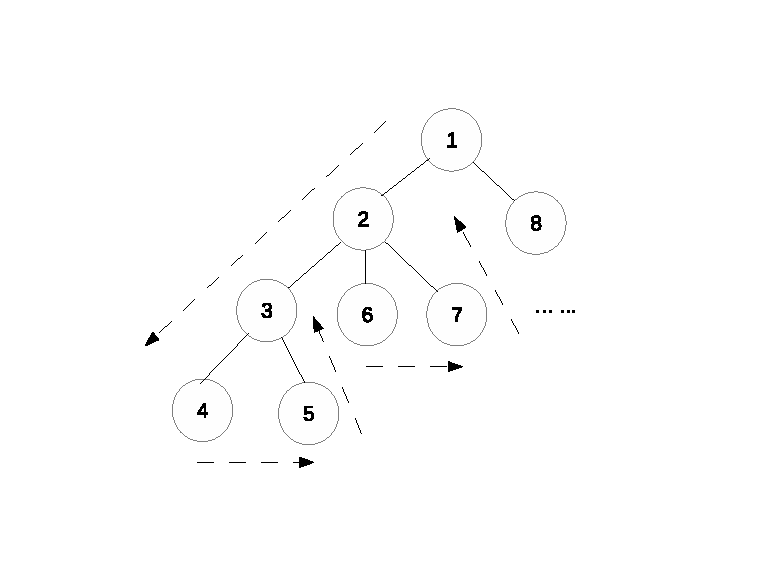
\includegraphics[scale=0.6]{img/dfs-tree.eps}
 \caption{深度优先搜索的顺序。}
 \label{fig:dfs-tree}
\end{figure}

这样的搜索策略称为深度优先搜索DFS(Deep-first-search)。在现实世界中,我们在不经意间广泛使用深度优先搜索。某些编程环境,例如Prolog,使用深度优先作为默认的求值模型。例如一个迷宫可以被一组规则描述:

\lstset{language=Prolog}
\begin{lstlisting}
c(a, b). c(a, e).
c(b, c). c(b, f).
c(e, d), c(e, f).
c(f, c).
c(g, d). c(g, h).
c(h, f).
\end{lstlisting}

其中,断言$c(X, Y)$表示位置$X$和$Y$连通。注意,这一断言是有方向性的。如果要让$Y$和$X$连通,我们可以增加一条对称的断言,或者建立一条无方向性的断音。图\ref{fig:directed-graph}给出了一个有向图。任意给出两个位置$X$和$Y$,Prolog可以通过下面的程序判定它们之间是否有通路。

\begin{figure}[htbp]
 \centering
 \includegraphics[scale=0.5]{img/directed-graph.ps}
 \caption{一个有向图。}
 \label{fig:directed-graph}
\end{figure}

\lstset{language=Prolog}
\begin{lstlisting}
go(X, X).
go(X, Y) :- c(X, Z), go(Z, Y)
\end{lstlisting}

这一程序说明,一个位置和自己相通。任意给出两个不同的位置$X$和$Y$,若$X$和$Z$相连,且$Z$和$Y$之间有通路,则$X$和$Y$之间存在通路。显然,$Z$的选择可能是不唯一的。Prolog会选择一个,然后继续进行搜索。只有当递归搜索失败时,才会尝试其他选择。此时,Prolog会回溯,并更换到下一个选项上。着恰好就是深度优先的搜索策略。

当我们只需要找到解,而并不关心找到最少步数的解时,深度优先搜索是很有效的方法。例如,迷宫问题中找出的第一个解并不一定是最短的路径。我们接下来将给出更多的趣题,并给出找出最少步数解的方法。

\subsubsection{狼、羊、白菜趣题}
\index{The wolf, goat, and cabbage puzzle}

这是一道传统趣题。有一个农夫,带着一只狼、一只羊、和一筐白菜要过河。有一条小船,只有农夫会划船。由于船很小,只能装下农夫和另外一样东西。农夫每次只能在狼、羊、白菜中任选一样和他一起过河。但是如果农夫不在,狼会吃掉羊,而羊会吃掉白菜。这道题目要求找到最快的一种方法,可以让所有的东西都渡过河。

\begin{figure}[htbp]
 \centering
 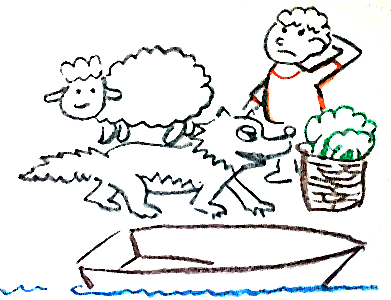
\includegraphics[scale=0.3]{img/wgc-puzzle.eps}
 \caption{狼、羊、白菜问题。}
 \label{fig:wgc-puzzle}
\end{figure}

这道题目的关键是狼不会吃掉白菜。因此农夫可以安全地将羊运到河对岸,并返回。但是接下来,无论他将狼或白菜中的任何一样运过河,他必须将某一样运回以避免有东西被吃掉。为了寻找最快的解法,只要存在多种选择,我们可以并发检查所有的选项,比较哪个会更快。如果不考虑渡河的方向,只要渡过一次,就算做一步,往返算两步,我们实际上在检查渡河一次后的所有可能、渡河两次后所有可能、三次后的所有可能……直到某次后,我们发现所有的东西都到达了河对岸,这一过程结束。并且这一渡河方法在所有可能中胜出,是最快的解法。

问题在于,我们无法真正并发检查所有可能的解法。除非使用带有多个CPU内核的超级计算机,但是对于解决这样一道简单的趣题,这相当于“高射炮打蚊子”。

让我们考虑一个抽奖游戏。游戏参与者不能看,闭着眼睛从一个箱子里掏出一个球。箱子里只有一个黑色球,其余的球都是白色的。摸到黑球的人获胜;如果摸到白球,他必须把球放回箱子,然后等待下次摸球。为了使得游戏公平,我们可以指定这样一个规则:必须等待所有其他人都摸过之后,才能再摸第二次。我们可以让参与游戏的人站成一队。每次站在队伍前面的人摸球,如果他没有摸到黑球获胜,他就站到队尾等待下次摸球。这一队列可以保证游戏的公平规则。

\begin{figure}[htbp]
 \centering
 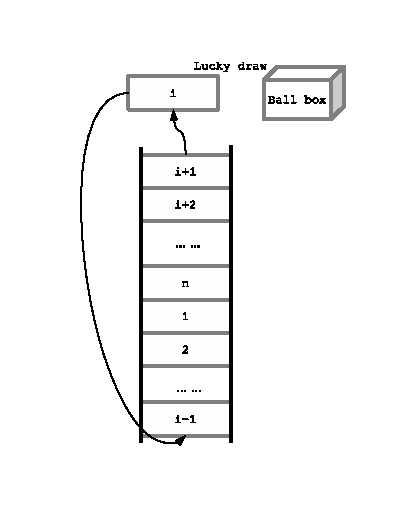
\includegraphics[scale=1]{img/lucky-draw.eps}
 \caption{抽奖游戏,第$i$个人出队,摸球。如果没有摸到黑球,就站到队尾。}
 \label{fig:luck-draw}
\end{figure}

我们可以用类似的思路来解决狼、羊、白菜趣题。河的两岸可以用两个集合$A$和$B$代表。开始的时候,集合$A$中包含狼、羊、白菜、和农夫;而集合$B$是空集。我们每次将农夫和另外一个元素从一个集合移动到另一个集合。每个集合中,如果不存在农夫,则不能含有相互冲突的东西。目标是用最少的次数,交换$A$和$B$的内容。

我们使用一个队列,最开始只包含一个状态$A = \{w, g, c, p\}$、$B=\phi$。只要队列不为空,我们就取出队列头部的元素,将其扩展为所有可能的选择,然后将扩展后的候选状态放回队列尾部。如果队列头部的第一个元素就是最终的目标,即$A=\phi$、$B=\{w, g, c, p\}$,我们就找到了解。图\ref{fig:bfs-tree}描述了这一思路的搜索顺序。同一深度上的所有可能性都被检查了,因此无需进行回溯。

\begin{figure}[htbp]
 \centering
 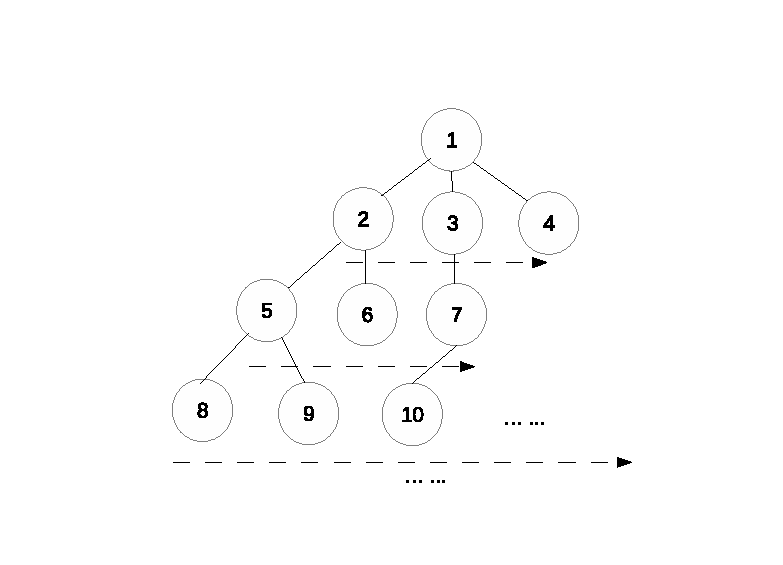
\includegraphics[scale=0.5]{img/bfs-tree.eps}
 \caption{从第一个状态开始,检查第二步的所有选项2、3、和4;然后检查第3层上的所有选项……}
 \label{fig:bfs-tree}
\end{figure}

我们可以用一个4位二进制数来表示集合,每一位表示一种事物,例如狼$w=1$、羊$g=2$、白菜$c=4$、农夫$p=8$。0表示空集合,15表示包含所有事物的集合。值3表示只有狼和羊被留在了河的这一侧。此时狼会吃掉羊。同样,值6表示另外一种存在冲突的情况。每次我们将最高位(值为8)和另外一位(4、2、或1)从一个数字移动到另外一个数字上。可行的移动方法定义如下:

\be
mv(A, B) = \left \{
  \begin{array}
  {r@{\quad:\quad}l}
  \{(A - 8 - i, B + 8 + i) | i \in \{0, 1, 2, 4\}, i = 0 \lor A \overline{\land} i \neq 0 \} & B < 8 \\
  \{(A + 8 + i, B - 8 - i) | i \in \{0, 1, 2, 4\}, i = 0 \lor B \overline{\land} i \neq 0 \} & Otherwise
  \end{array}
\right.
\ee

其中$\overline{\land}$表示按位与运算。

我们可以使用前面章节定义的纯函数式队列。记队列为$Q$,最开始队列包含一个列表,列表只含有一对元素\{(15, 0)\}。若$Q$不为空,则函数$DeQ(Q)$取出队列的头部元素$M$,队列中的剩余元素记为$Q'$。$M$为包含若干对元素的列表,代表在河岸间的一系列移动。表中第一个元素为$m_1=(A', B')$,是最后一次移动后的状态。函数$EnQ'(Q, L)$,是一个稍作改动的入队操作。它将$L$中所有可能的移动序列,逐一加入到队列的尾部,并返回新的队列。使用这些记号,寻找解的算法可以定义为如下的函数。

\be
solve(Q) = \left \{
  \begin{array}
  {r@{\quad:\quad}l}
  \phi & Q = \phi \\
  reverse(M) & A' = 0 \\
  solve(EnQ'(Q', \left \{
    \begin{array}{rl}
      \{m\} \cup M | & m \in mv(m_1), \\
                     & valid(m, M)
    \end{array}
    \right \})) & otherwise
  \end{array}
\right.
\ee

其中函数$valid(m, M)$检查新的移动结果$m=(A'', B'')$是否不存在冲突。它要求$A''$和$B''$即不能是3,也不能是6,并且$m$以前没有尝试过,它不存在于$M$中,以避免重复的尝试。

\be
valid(m, M) = A'' \neq 3, A'' \neq 6, B'' \neq 3, B'' \neq 6, m \notin M
\ee

下面的Haskell例子程序实现了狼、羊、白菜问题的解法。为了简单,这里我们使用了普通的列表来表示队列。严格来说应该使用前面章节介绍过的纯函数式队列。

\lstset{language=Haskell}
\begin{lstlisting}
import Data.Bits

solve = bfsSolve [[(15, 0)]] where
    bfsSolve :: [[(Int, Int)]] -> [(Int, Int)]
    bfsSolve [] = [] -- no solution
    bfsSolve (c:cs) | (fst $ head c) == 0 = reverse c
                    | otherwise = bfsSolve (cs ++ map (:c)
                                      (filter (`valid` c) $ moves $ head c))
    valid (a, b) r = not $ or [ a `elem` [3, 6], b `elem` [3, 6],
                                (a, b) `elem` r]

moves (a, b) = if b < 8 then trans a b else map swap (trans b a) where
    trans x y = [(x - 8 - i, y + 8 + i)
                     | i <-[0, 1, 2, 4], i == 0 || (x .&. i) /= 0]
    swap (x, y) = (y, x)
\end{lstlisting}

可以对这一算法稍作改动,找出所有可能的解,而不是在找出最快的解后结束。作为练习,读者可以尝试这一改动。下面给出了狼、羊、白菜问题的两个最优解。

第一个解:

\begin{tabular}{l|c|l}
Left & river & Right \\
\hline
wolf, goat, cabbage, farmer &   & \\
wolf, cabbage &   & goat, farmer \\
wolf, cabbage, farmer &   & goat \\
cabbage &   & wolf, goat, farmer \\
goat, cabbage, farmer &   & wolf \\
goat &   & wolf, cabbage, farmer \\
goat, farmer &   & wolf, cabbage \\
 &  & wolf, goat, cabbage, farmer
\end{tabular}

第二个解:

\begin{tabular}{l|c|l}
Left & river & Right \\
\hline
 wolf, goat, cabbage, farmer & & \\
 wolf, cabbage & & goat, farmer \\
 wolf, cabbage, farmer & & goat \\
 wolf & & goat, cabbage, farmer \\
 wolf, goat, farmer & & cabbage \\
 goat & & wolf, cabbage, farmer \\
 goat, farmer & & wolf, cabbage \\
 & & wolf, goat, cabbage, farmer
\end{tabular}

这一问题也可以用命令式的方式解决。观察可以发现我们的解是尾递归的,我们可以将它直接转换为循环。我们使用列表$S$来记录所有找到的解。一开始把只含有一个元素的表$\{(15, 0)\}$放入队列。只要队列不为空,我们就调用过程\textproc{DeQ}从头部取出元素$C$。检查是否到达了最终的目标状态,如果没有,就展开所有可能的移动选项,并将它们加入回队列的尾部,以便后继的搜索。

\begin{algorithmic}[1]
\Function{Solve}{}
  \State $S \gets \phi$
  \State $Q \gets \phi$
  \State \Call{EnQ}{$Q, \{(15, 0)\}$}
  \While{$Q \neq \phi$}
    \State $C \gets $ \Call{DeQ}{$Q$}
    \If{$c_1 = (0, 15)$}
      \State \textproc{Add}($S$, \Call{Reverse}{$C$})
    \Else
      \For{$\forall m \in $ \Call{Moves}{$C$}}
        \If{\Call{Valid}{$m, C$}}
          \State \Call{EnQ}{$Q, \{m\} \cup C$}
        \EndIf
      \EndFor
    \EndIf
  \EndWhile
  \State \Return $S$
\EndFunction
\end{algorithmic}

其中过程\textproc{Moves}和\textproc{Valid}的定义与此前相同。下面的Python例子程序实现了狼、羊、白菜问题的解法。

\lstset{language=Python}
\begin{lstlisting}
def solve():
    s = []
    queue = [[(0xf, 0)]]
    while queue != []:
        cur = queue.pop(0)
        if cur[0] == (0, 0xf):
            s.append(reverse(cur))
        else:
            for m in moves(cur):
                queue.append([m]+cur)
    return s

def moves(s):
    (a, b) = s[0]
    return valid(s, trans(a, b) if b < 8 else swaps(trans(b, a)))

def valid(s, mv):
    return [(a, b) for (a, b) in mv
        if a not in [3, 6] and b not in [3, 6] and (a, b) not in s]

def trans(a, b):
    masks = [ 8 | (1<<i) for i in range(4)]
    return [(a ^ mask, b | mask) for mask in masks if a & mask == mask]

def swaps(s):
    return [(b, a) for (a, b) in s]
\end{lstlisting}

这一程序和前面的算法描述略有不同,它在产生可能的移动选项时,同时去掉了含有冲突的情况。

每次农夫渡河时,他都有$m$个可能的选择,其中$m$是农夫所在的河岸上事物的数目。$m$总小于4,因此算法在第$n$次渡河时的运行时间不会超过$n^4$。这一估计远远超过实际的时间,我们避免尝试所有含有冲突或重复的情况。最坏情况下,我们的算法会检查所有可能到达的状态。由于需要检查记录以避免重复,算法大约使用$O(n^2)$的时间来搜索第$n$次渡河时的所有可能状态。

\subsubsection{倒水问题}
\index{Water jugs puzzle}

倒水问题是一道经典人工智能中的著名趣题。这一问题的历史悠久。只有两个水瓶,一个的容量是9升水,另一个的容量是4升水。问如何才能从河中取出6升水?

这道题目有很多变化形式,瓶子的容积和要取出的水的容量可以是其他数值。有一个故事说解决这道题目的主人公是少年时代的法国数学家和科学家帕斯卡(Blaise Pascal),另一故事说是泊松(Sim\`{e}on Denis Poisson)。在著名的好莱坞电影《虎胆龙威3》(Die-Hard 3)中,电影明星布鲁斯,威利斯(Bruce Willis)和塞缪尔,杰克逊(Samuel L. Jackson)也遇到了同样的趣题。

著名的数学家波利亚(P\`{o}lya)在《如何解题》中给出了一个倒推法的解\cite{how-to-solve-it}。

\begin{figure}[htbp]
 \centering
 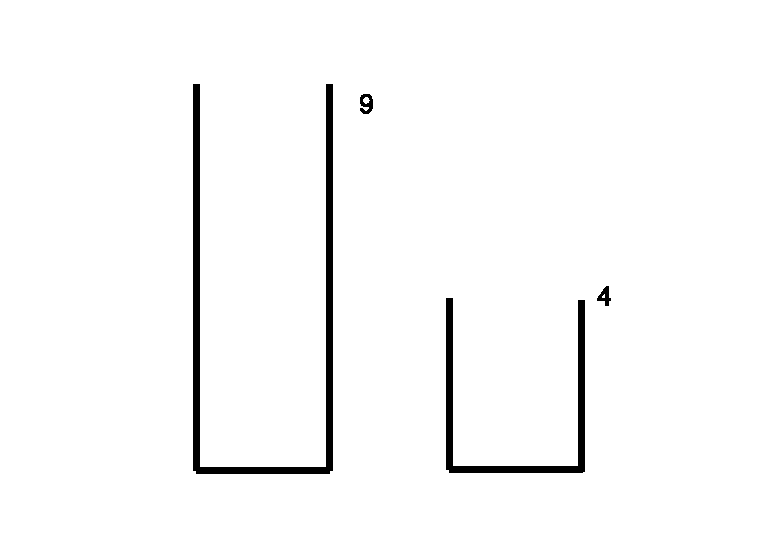
\includegraphics[scale=0.5]{img/jugs-start.eps}
 \caption{两个瓶子的容积分别为9和4。}
 \label{fig:jugs-start}
\end{figure}

从图\ref{fig:jugs-start}的起始状态思考会比较困难。波利亚指出,最终的状态是,大瓶子中盛有6升水。这样我们可以得知,前一步时,我们从9升的大瓶子中倒出3升水。为了达成这一点,小瓶子中需要盛有1升水。如图\ref{fig:jugs-r1}所示。

\begin{figure}[htbp]
 \centering
 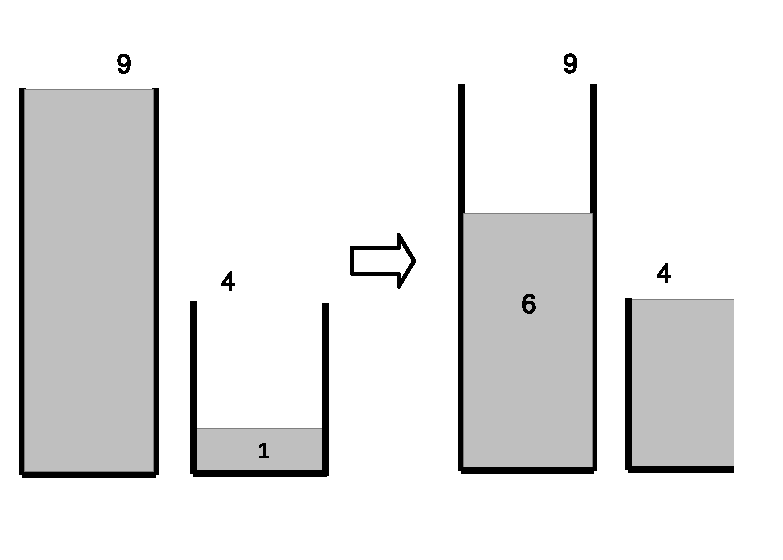
\includegraphics[scale=0.5]{img/jugs-r1.eps}
 \caption{最后两步}
 \label{fig:jugs-r1}
\end{figure}

很容易看出,只要倒满9升的瓶子,然后连续两次倒入4升的瓶子,并将4升的瓶子倒空,就可以得到1升水。如图\ref{fig:jugs-r2}所示。此时,我们已经找到解了。通过倒推法,我们可以比较容易地得到6升水的获取方法。

\begin{figure}[htbp]
 \centering
 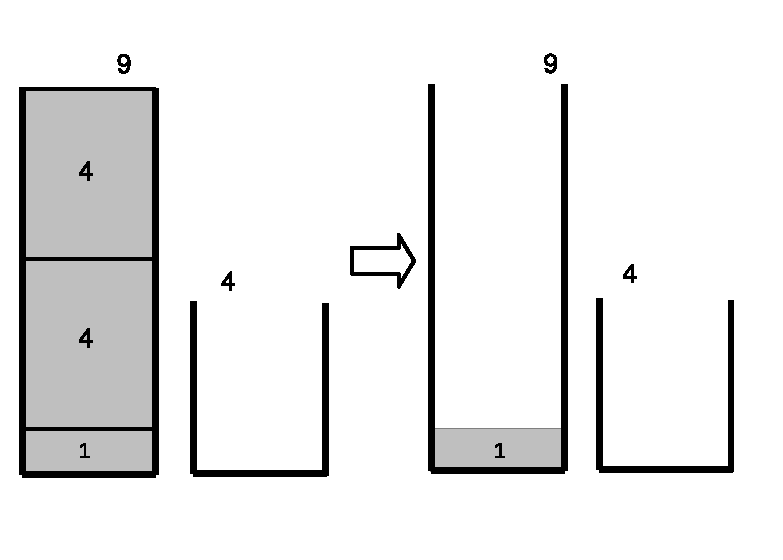
\includegraphics[scale=0.5]{img/jugs-r2.eps}
 \caption{将大瓶倒满,然后倒入小瓶两次。}
 \label{fig:jugs-r2}
\end{figure}

波利亚的方法是一种策略性的通用方法。但是仍然无法直接从中得到具体的算法。例如怎样从899升和1147升的瓶子得到2升水?

使用两个瓶子,每次有6种操作方法。记小瓶子为$A$,大瓶子为$B$:

\begin{itemize}
\item 将小瓶子$A$装满水;
\item 将大瓶子$B$装满水;
\item 将小瓶子$A$中的水倒空;
\item 将大瓶子$B$中的水倒空;
\item 将小瓶子$A$中的水倒入大瓶子$B$;
\item 将大瓶子$B$中的水倒入小瓶子$A$。
\end{itemize}

下面的是一系列倒水的动作,这里我们假设容积$a < b < 2a$。

\begin{tabular}{l|l|l}
$A$ & $B$ & 操作 \\
\hline
0 & 0 & 开始 \\
a & 0 & 倒满$A$ \\
0 & a & 将$A$倒入$B$ \\
a & a & 倒满$A$ \\
2a - b & b & 将$A$倒入$B$ \\
2a - b & 0 & 倒光$B$ \\
0 & 2a - b & 将$A$倒入$B$ \\
a & 2a - b & 倒满$A$ \\
3a - 2b & b & 将$A$倒入$B$ \\
... & ... & ... \\
\end{tabular}

无论进行何种操作,每个瓶子中的水的容量总可以表示为$xa + yb$的形式,其中$a$和$b$分别是两个瓶子的容量,$x$和$y$是整数。也就是说,我们能获得的水的体积总是$a$与$b$的线性组合。于是我们立即可以知道,给定两个瓶子的容量,是否可以得到$g$升的水。

例如,使用两个分别容量为4升和6升的瓶子,我们永远无法得到5升的水。通过使用数论中的定理可知,使用两个瓶子,当且仅当$g$能够被瓶子容积的最大公约数整除时,才能得到$g$升水。即:

\be
gcd(a, b) | g
\ee

其中$ m | n $表示整数$n$可以被$m$整除。进一步说,如果$a$和$b$互素,即$gcd(a, b) = 1$,则可以得到任意自然数$g$升水。

虽然通过检查$gcd(a, b)$是否整除$g$可以判断问题是否有解,但是我们并不知道解的具体倒水操作顺序。如果我们可以找到整数$x$和$y$,使得$g = xa + yb$。就可以得到一组操作(尽管可能不是最优解)来解决此题。具体思路是这样的:不失一般性,设$x > 0, y < 0$,我们需要倒满瓶子$A$总共$x$次,倒空瓶子$B$总共$y$次。

例如,若小瓶容积$a=3$、大瓶容积$b=5$,要取得$g=4$升水,因为$4 = 3 \times 3 - 5$,我们可以设计下面的一系列操作:

\begin{tabular}{l|l|l}
$A$ & $B$ & 操作 \\
\hline
0 & 0 & 开始 \\
3 & 0 & 倒满$A$ \\
0 & 3 & 将$A$倒入$B$ \\
3 & 3 & 倒满$A$ \\
1 & 5 & 将$A$倒入$B$ \\
1 & 0 & 将$B$倒空 \\
0 & 1 & 将$A$倒入$B$ \\
3 & 1 & 倒满$A$ \\
0 & 4 & 将$A$倒入$B$ \\
\end{tabular}

在这一系列操作中,我们倒满$A$共3次,倒空$B$共1次。这一过程可以描述如下。

重复$x$次:
\begin{enumerate}
\item 倒满$A$;
\item 将$A$倒入$B$,若$B$变满,则将其倒空。
\end{enumerate}

因此剩下的唯一问题是寻找整数$x$和$y$。数论中有一个强大的工具叫做\underline{扩展欧几里得算法}(Extended Euclid algorithm),可以用来解决这个问题。经典的欧几里得算法,只能找到最大公约数,而扩展欧几里得算法还可以同时得到一对整数$x$和$y$,使得:

\be
(d, x, y) = gcd_{ext}(a, b)
\ee

其中$d = gcd(a, b)$为最大公约数,而$ax + by = d$。不失一般性,设$a < b$,存在商$q$和余数$r$使得:

\be
b = a q + r
\ee

因为$d$是公约数,他可以同时整除$a$和$b$,因此$d$也可以整除$r$。由于$r$小于$a$,我们可以通过寻找$a$和$r$的最大公约数来减小问题的规模。

\be
(d, x', y') = gcd_{ext}(r, a)
\label{eq:recursive-ext-gcd}
\ee

根据扩展欧几里得算法的定义,其中$d = x' r + y' a$。将$b = a q + r$转换为$r = b - a q$并替换上式中的$r$,可以得到:

\be
\begin{array}{rcl}
d & = & x' (b - a q) + y' a \\
  & = & (y' - x' q) a + x' b
\end{array}
\ee

这正好是$a$与$b$的线性组合,于是我们有:

\be
\left \{
  \begin{array}{l}
  x = y' - x' \displaystyle \frac{b}{a} \\
  y = x'
  \end{array}
\right.
\ee

这是一个典型的递归关系。边界条件发生在$a=0$时。

\be
gcd(0, b) = b = 0 a + 1 b
\ee

综上,扩展欧几里得算法可以定义如下:

\be
gcd_{ext}(a, b) = \left \{
  \begin{array}
  {r@{\quad:\quad}l}
  (b, 0, 1) & a = 0 \\
  (d, y' - x' \displaystyle \frac{b}{a}, x') & otherwise
  \end{array}
\right.
\ee

其中$d$、$x'$、$y'$的定义如式(\ref{eq:recursive-ext-gcd})。

倒水问题几乎解决了,但是我们仍需处理两个具体的问题。第一、扩展欧几里得算法给出了最大公约数及其线性组合。但要取水的容量$g$可能不等于$d$,而是$d$的倍数。若$m = g / gcd(a, b)$,我们可以分别将$x$和$y$乘以$m$倍;第二、我们假设$x>0$,来设计了倒满瓶子$A$总共$x$的过程。但扩展欧几里得算法并不保证$x$为正数。例如$gcd_{ext}(4, 9) = (1, -2, 1)$。若$x$为负数,由于$d = x a + y b$,我们可以不断将$x$加$b$,同时将$y$减$a$,直到$x$大于0。

至此,我们已可以给出完整的两瓶倒水问题的解了。下面的Haskell例子程序实现了这一解法。

\lstset{language=Haskell}
\begin{lstlisting}
extGcd 0 b = (b, 0, 1)
extGcd a b = let (d, x', y') = extGcd (b `mod` a) a in
               (d, y' - x' * (b `div` a), x')

solve a b g | g `mod` d /= 0 = [] -- no solution
            | otherwise = solve' (x * g `div` d)
    where
      (d, x, y) = extGcd a b
      solve' x | x < 0 = solve' (x + b)
               | otherwise = pour x [(0, 0)]
      pour 0 ps = reverse ((0, g):ps)
      pour x ps@((a', b'):_) | a' == 0 = pour (x - 1) ((a, b'):ps) -- fill a
                             | b' == b = pour x ((a', 0):ps) -- empty b
                             | otherwise = pour x ((max 0 (a' + b' - b),
                                                    min (a' + b') b):ps)
\end{lstlisting}

虽然我们可以用扩展欧几里得算法解决两瓶倒水问题,但是得到的解并不一定是最优的。例如,使用3升和5升的瓶子,获取4升水的时候,扩展欧几里得算法给出如下的操作顺序:

\begin{verbatim}
[(0,0),(3,0),(0,3),(3,3),(1,5),(1,0),(0,1),(3,1),
(0,4),(3,4),(2,5),(2,0),(0,2),(3,2),(0,5),(3,5),
(3,0),(0,3),(3,3),(1,5),(1,0),(0,1),(3,1),(0,4)]
\end{verbatim}

总共需要23步,而最优解只需要6步:

\begin{verbatim}
[(0,0),(0,5),(3,2),(0,2),(2,0),(2,5),(3,4)]
\end{verbatim}

观察23步的解,我们发现在第8步时,瓶子$B$中已有4升水了。但是算法仍然继续执行后面的15步。原因是我们通过扩展欧几里得算法得到的线性组合$x$和$y$并非满足条件的唯一线性组合。在所有满足$g = x a + b y$的整数中,$|x| + |y|$越小,所需步骤越少。本章附带的练习中有一道题目要求寻找最优的线性组合。

如何寻找最优解?我们有两种策略,一种是寻找$x$和$y$,使得$|x| + |y|$最小;另外一种是采用“狼、羊、白菜问题”的思路。本节我们介绍后一种方法。由于我们最多有6种可能的操作:倒满$A$、倒满$B$、将$A$倒入$B$、将$B$倒入$A$、倒空$A$、和倒空$B$,我们可以并行尝试所有的操作,检查那个操作可以得到最优解。我们需要记录所有已经到达的状态以避免重复。为了用有限的资源获得并行的效果,我们使用一个队列来安排所有的尝试。队列中保存的元素是一系列值对$(p, q)$,其中$p$和$q$分别是两个瓶中盛水的体积。这些值对记录了从开始到最后进行的倒水操作。队列一开始时,唯一的元素是一个列表。表中含有一对值$\{ (0, 0) \}$。

\be
solve(a, b, g) = solve' \{ \{ (0, 0) \} \}
\ee

只要队列不为空,我们就从队列头部取出一个操作序列,如果这一序列中的组后一个状态,包含目标容量$g$升水,则我们找到了一个解,我们将这一序列逆序输出;否则,我们扩展最后一个状态,尝试所有6种可能,去掉重复的状态,并将它们加入到队列尾部。记队列为$Q$,队列头部保存的序列为$S$,$S$中最后一对值为$(p, q)$,剩下的其余对胃$S'$。头部元素出队后,队列变为$Q'$。这一搜索算法可定义如下:

\be
solve'(Q) = \left \{
  \begin{array}
  {r@{\quad:\quad}l}
  \phi & Q = \phi \\
  reverse(S) & p = g \lor q = g \\
  solve'(EnQ'(Q', \{\{s'\} \cup S' | s' \in try(S)\})) & otherwise
  \end{array}
\right.
\ee

其中函数$EnQ'$逐一将列表中的序列加入到队尾。函数$try(S)$尝试所有6种操作,并产生新的水的体积对:

\be
try(S) = \{s' | s' \in \left \{ \begin{array}{l}
  fillA(p, q), fillB(p, q), \\
  pourA(p, q), pourB(p, q), \\
  emptyA(p, q), emptyB(p, q)
  \end{array}
  \right \}, s' \notin S' \}
\ee

6种操作的定义很直观。对于倒满操作,结果是水瓶中水的体积达到瓶子的容积;对于倒空操作,瓶中水的体积为0;对于倒入操作,我们需要检查目标瓶子的剩余容量是否足够大。

\be
\begin{array}{ll}
fillA(p, q) = (a, q) & fillB(p, q) = (p, b) \\
emptyA(p, q) = (0, q) & emptyB(p, q) = (p, 0) \\
pourA(p, q) = (max(0, p + q - b), min(x + y, b)) & \\
pourB(p, q) = (min(x + y, a), max(0, x + y - a)) &
\end{array}
\ee

下面的Haskell程序实现了这一解法。

\lstset{language=Haskell}
\begin{lstlisting}
solve' a b g = bfs [[(0, 0)]] where
  bfs [] = []
  bfs (c:cs) | fst (head c) == g || snd (head c) == g = reverse c
             | otherwise = bfs (cs ++ map (:c) (expand c))
  expand ((x, y):ps) = filter (`notElem` ps) $ map (\f -> f x y)
                           [fillA, fillB, pourA, pourB, emptyA, emptyB]
  fillA _ y = (a, y)
  fillB x _ = (x, b)
  emptyA _ y = (0, y)
  emptyB x _ = (x, 0)
  pourA x y = (max 0 (x + y - b), min (x + y) b)
  pourB x y = (min (x + y) a, max 0 (x + y - a))
\end{lstlisting} %$

这一方法总返回最快的解法。它也可以用命令式的方法实现。我们无需在队列的每个元素中保存全部的操作序列,可以建立一个全局的历史记录列表,然后使用指针链接操作的顺序。这样能节省大量的空间。

\begin{figure}[htbp]
  \centering
  \includegraphics[scale=0.5]{img/water-jugs.ps}
  \caption{所有尝试过的状态都存储与一个全局的列表中。}
  \label{fig:water-jugs}
\end{figure}

如图\ref{fig:water-jugs}所示,初始状态为(0, 0)。只有`fill A'和`fill B'可行。它们被加入记录;接下来,我们在记录的结果(3, 0)的基础上尝试`fill B',并将新结果(3, 5)记录下来。但是在(3, 0)的基础上尝试`empty A'将回到初始状态(0, 0)。由于我们已记录了这一状态,所以这一选项被跳过。图中,所有灰色的状态,都是重复状态。

通过这样的设计,我们无需在队列的每个元素中记录操作的序列。我们可以给图\ref{fig:water-jugs}中的每个节点增加一个父节点指针,并用它从任意状态回溯到初始状态。下面的C语言例子代码给出了这一设计的定义。

\lstset{language=C}
\begin{lstlisting}
struct Step {
    int p, q;
    struct Step* parent;
};

struct Step* make_step(int p, int q, struct Step* parent) {
    struct Step* s = (struct Step*) malloc(sizeof(struct Step));
    s->p = p;
    s->q = q;
    s->parent = parent;
    return s;
}
\end{lstlisting}

其中$p$和$q$是两个水平中盛水的体积。对于任何状态$s$,定义函数$p(s)$和$q(s)$分别返回这两个量,命令式算法可以实现如下:

\begin{algorithmic}[1]
\Function{Solve}{$a, b, g$}
  \State $Q \gets \phi$
  \State \Call{Push-and-record}{$Q$, (0, 0)}
  \While{$Q \neq \phi$}
    \State $s \gets$ \Call{Pop}{$Q$}
    \If{$p(s) = g \lor q(s) = g$}
      \State \Return $s$
    \Else
      \State $C \gets$ \Call{Expand}{$s$}
      \For{$\forall c \in C$}
        \If{$c \neq s \land \lnot$ \Call{Visited}{$c$}}
          \State \Call{Push-and-record}{$Q, c$}
        \EndIf
      \EndFor
    \EndIf
  \EndWhile
  \State \Return NIL
\EndFunction
\end{algorithmic}

其中\textproc{Push-and-record}不仅将元素加入队列尾部,还将其记录入访问过的状态的表中,这样将来就可以检查是否到达过此状态。所有的push操作都将新元素加入到列表的尾部。对于pop操作,我们并不将元素删除,而是将头指针向后移动一步。这一包含所有历史数据的列表必须在使用前清空。下面的C语言例子程序实现了这一算法。

\lstset{language=C}
\begin{lstlisting}
struct Step *steps[1000], **head, **tail = steps;

void push(struct Step* s) { *tail++ = s; }

struct Step* pop() { return *head++; }

int empty() { return head == tail; }

void reset() {
    struct Step **p;
    for (p = steps; p != tail; ++p)
        free(*p);
    head = tail = steps;
}
\end{lstlisting}

为了检查一个状态是否访问过,我们需要遍历列表,比较$p$和$q$的值。

\lstset{language=C}
\begin{lstlisting}
int eq(struct Step* a, struct Step* b) {
    return a->p == b->p && a->q == b->q;
}

int visited(struct Step* s) {
    struct Step **p;
    for (p = steps; p != tail; ++p)
        if (eq(*p, s)) return 1;
    return 0;
}
\end{lstlisting}

主程序实现如下:

\lstset{language=C}
\begin{lstlisting}
struct Step* solve(int a, int b, int g) {
    int i;
    struct Step *cur, *cs[6];
    reset();
    push(make_step(0, 0, NULL));
    while (!empty()) {
        cur = pop();
        if (cur->p == g || cur->q == g)
            return cur;
        else {
            expand(cur, a, b, cs);
            for (i = 0; i < 6; ++i)
                if(!eq(cur, cs[i]) && !visited(cs[i]))
                    push(cs[i]);
        }
    }
    return NULL;
}
\end{lstlisting}

其中函数\texttt{expand}尝试所有6种操作:

\lstset{language=C}
\begin{lstlisting}
void expand(struct Step* s, int a, int b, struct Step** cs) {
    int p = s->p, q = s->q;
    cs[0] = make_step(a, q, s); /*fill A*/
    cs[1] = make_step(p, b, s); /*fill B*/
    cs[2] = make_step(0, q, s); /*empty A*/
    cs[3] = make_step(p, 0, s); /*empty B*/
    cs[4] = make_step(max(0, p + q - b), min(p + q, b), s); /*pour A*/
    cs[5] = make_step(min(p + q, a), max(0, p + q - a), s); /*pour B*/
}
\end{lstlisting}

结果步骤可以通过父指针不断向上逆序输出,如下面的递归函数实现:

\lstset{language=C}
\begin{lstlisting}
void print(struct Step* s) {
    if (s) {
        print(s->parent);
        printf("%d, %d\n", s->p, s->q);
    }
}
\end{lstlisting}

\subsubsection{华容道}
\index{Kloski puzzle}

华容道是一种滑块类游戏,国外称Kloski。在很多国家都有类似的游戏。滑块的大小和布局会有不同。图\ref{fig:klotski-cn}中是传统的华容道游戏。

\begin{figure}[htbp]
 \centering
 \subfloat[起始布局]{\includegraphics[scale=0.5]{img/klotski-cn1.eps}} \hspace{.01\textwidth}
 \subfloat[移动若干步后的样子]{\includegraphics[scale=0.5]{img/klotski-cn2.eps}}
 \caption{华容道游戏}
 \label{fig:klotski-cn}
\end{figure}

华容道游戏中,共有10个滑块,每个上面标有数字或者图案。最小的滑块大小为一个单位的正方形,最大的一块为$2 \times 2$单位。在棋盘下方的中间,有一个宽度为2个单位长的缺口。最大的一块代表曹操,其他的为刘备手下的五虎上将和士兵。游戏的目标是要通过滑动,将曹操移动到棋盘最下方逃走。图\ref{fig:klotski-jp}是日本的类似游戏,名叫“箱子中的女儿”,最大的一块代表女儿,剩余滑块代表其他家庭成员。

\begin{figure}[htbp]
 \centering
 \includegraphics[scale=0.5]{img/klotski-jp.eps}
 \caption{日本的“箱子中的女儿”游戏}
 \label{fig:klotski-jp}
\end{figure}

本节中,我们要找出一种解法,通过一系列移动,用最少的步数,将滑块从初始状态,变换到目标状态。

最直观的想法,是用一个$5 \times 4$矩阵来代表棋盘。每个棋子被标记为一个数字。下面的矩阵$M$,给出了华容道的初始状态。

\[
M = \left [
  \begin{array}{cccc}
  1 & 10 & 10 & 2 \\
  1 & 10 & 10 & 2 \\
  3 & 4 & 4 & 5 \\
  3 & 7 & 8 & 5 \\
  6 & 0 & 0 & 9
  \end{array}
\right ]
\]

在矩阵中,值为$i$的元素表示相应的位置被第$i$个棋子所占。特殊值0代表空位置。通过使用序列1、2、……来代表棋子,一个布局可以进一步用一个数组$L$来代表。每个元素是一个列表,包含若干被该元素所代表的棋子覆盖的所有位置。例如$L[4] = \{(3, 2), (3, 3)\}$表示,第4个棋子覆盖了位置$(3, 2)$和$(3, 3)$,其中$(i, j)$表示在第$i$行、第$j$列的位置。

华容道的初始布局可以用这种方法写成下面的数组。

\[
\begin{array}{l}
\{ \{(1, 1), (2, 1) \},
 \{(1, 4), (2, 4) \},
 \{(3, 1), (4, 1) \},
 \{(3, 2), (3, 3) \},
 \{(3, 4), (4, 4) \}, \\
 \{(5, 1) \},
 \{(4, 2) \},
 \{(4, 3) \},
 \{(5, 4) \},
 \{(1, 2), (1, 3), (2, 2), (2, 3) \} \}
\end{array}
\]

解华容道时,我们需要检查全部10个棋子,看看能否在上下左右4个方向移动。看起来这是一个巨大的解空间,每步都有$10 \times 4$个选项,走$n$步后,会有$40^n$种情况。但实际上的情况没有这么多。例如在第一步的时候,只有4种可能:将第6块向右移动;将第7块或第8块向下移动;以及将第9块向左移动。所有其他选项都不可能发生。图\ref{fig:klotski-valid-move}给出了检查某种移动是否可行的方法。

\begin{figure}[htbp]
 \centering
 \includegraphics[scale=0.4]{img/klotski-valid-move.eps}
 \caption{左侧:两个标为1的格子都可以移动;右侧:上方标为1的格子虽然可以,但是下方标为1的格子和标为2的格子冲突。}
 \label{fig:klotski-valid-move}
\end{figure}

左侧的例子描述了将标为1的棋子向下滑动一个单位的情况。这个棋子覆盖两个格子。上方的1要移动到的格子此前也被这个棋子所占,所以格子的值也为1;下方的1要移动到一个空格子,空格子标记为0;

右侧的例子描述了一个不可行的移动。这个例子中,虽然棋子上方的部分可以移动到一个被同样棋子所占的格子中,但是下方部分的1不能移动到被其他棋子2所占的格子中。

为了确定一个移动是否合法,我们需要检查棋子覆盖的所有格子将要移动到的位置,如果目标位置的格子为0,或者比较数字相同,移动就是可行的。否则就会和其他棋子冲突。对于布局$L$,对应的矩阵为$M$,设我们要移动第$k$个棋子,移动方向为$(\Delta x, \Delta y)$,其中$|\Delta x| \leq 1$、$|\Delta y| \leq 1$。下面的等式,定义了移动是否可行:

\be
\begin{array}{rl}
valid(L, k, \Delta x, \Delta y): & \\
\forall (i, j) \in L[k] \Rightarrow & i' = i + \Delta y, j' = j + \Delta x, \\
& (1, 1) \leq (i', j') \leq (5, 4), M_{i'j'} \in \{k, 0\}
\end{array}
\ee

解决华容道问题的另一个重点是如何避免重复的尝试。经过一系列的移动,我们可能会回到此前的某个布局。但是,仅仅避免出现相同的矩阵是不够的,考虑下面给出的两个矩阵,虽然$M_1 \neq M_2$,但是我们仍然要避免移动到$M_2$,因为他们本质上是相同的。

\[
\begin{array}{cc}
M_1 = \left [
  \begin{array}{cccc}
  1 & 10 & 10 & 2 \\
  1 & 10 & 10 & 2 \\
  3 & 4 & 4 & 5 \\
  3 & 7 & 8 & 5 \\
  6 & 0 & 0 & 9
  \end{array}
\right ] &
M_2 = \left [
  \begin{array}{cccc}
  2 & 10 & 10 & 1 \\
  2 & 10 & 10 & 1 \\
  3 & 4 & 4 & 5 \\
  3 & 7 & 6 & 5 \\
  8 & 0 & 0 & 9
  \end{array}
\right ]
\end{array}
\]

这一事实告诉我们,需要比较布局,而不仅仅是矩阵来避免出现重复。记上述矩阵对应的布局分别为$L_1$和$L_2$,可以很容易验证$||L_1|| = ||L_2||$,其中$||L||$是归一化的布局,其定义如下:

\be
||L|| = sort(\{sort(l_i) | \forall l_i \in L\})
\ee

归一化的布局中,所有的元素都排好序,并且每个元素内部也都是有序的。相互间的顺序定义为:$(a, b) \leq (c, d) \Leftrightarrow a n + b \leq c n + d$,其中$n$是矩阵的宽度。

观察到华容道的棋盘是对称的,因此布局也可以有对称布局。出现对称的布局也是一种重复,我们需要避免它。例如下面的$M_1$和$M_2$就是对称的布局。

\[
\begin{array}{cc}
M_1 = \left [
  \begin{array}{cccc}
  10 & 10 & 1 & 2 \\
  10 & 10 & 1 & 2 \\
  3 & 5 & 4 & 4 \\
  3 & 5 & 8 & 9 \\
  6 & 7 & 0 & 0
  \end{array}
\right ] &
M_2 = \left [
  \begin{array}{cccc}
  3 & 1 & 10 & 10 \\
  3 & 1 & 10 & 10 \\
  4 & 4 & 2 & 5 \\
  7 & 6 & 2 & 5 \\
  0 & 0 & 9 & 8
  \end{array}
\right ]
\end{array}
\]

注意到他们的归一化布局也是相互对称的。通过下面方法可以很容易得到一个对称的布局。

\be
mirror(L) = \{\{(i, n - j + 1) | \forall (i, j) \in l \} | \forall l \in L \}
\ee

我们发现矩阵对于验证移动是否可行很方便,而布局形式便于表达移动和避免重复。我们可以用类似的方法来解决华容道游戏。使用一个队列,队列中的每个元素包含两部分:一系列移动,和这些移动导致的布局。每次移动的形式为$(k, (\Delta y, \Delta x))$,表示在棋盘上移动第$k$个棋子,$\Delta y$行和$\Delta x$列。

最开始的时候,队列中包含起始布局。只要队列不为空,我们就从队列头部取出一个元素,检查最大的一块棋子是否已经到达目标位置,即$L[10] = \{(4, 2), (4, 3), (5, 2), (5, 3)\}$。如果到达,则结束;否则,我们对每块棋子尝试向上下左右4个方向移动,并把所有可行的、不重复的布局存入队列尾部。在整个搜索过程中,我们需要保存所有找到的归一化布局以避免重复。

记队列为$Q$,布局的历史记录为$H$,队列头部记录的第一个布局为$L$,它对应的矩阵为$M$。到这个布局为止的一系列移动为$S$。下面的算法定义了华容道游戏的解法。

\be
solve(Q, H) = \left \{
  \begin{array}
  {r@{\quad:\quad}l}
  \phi & Q = \phi \\
  reverse(S) & L[10] = \{(4, 2), (4, 3), (5, 2), (5, 3)\} \\
  solve(Q', H') & otherwise
  \end{array}
\right.
\ee

第一行表示,如果队列为空,我们已经尝试了所有可能的移动方案,但是未能找到可行的解;第二行表示我们找到了一个解,我们将移动序列逆序返回;这两种是边界情况。否则,算法从当前的布局扩展出所有可行的移动方案,并将新布局加入到队列的尾部。新队列记为$Q'$,更新后的布局历史记录为$H'$。然后程序进行递归搜索。

为了将一个布局扩展为不重复的新布局,我们定义了如下的函数:

\be
\begin{array}{rl}
expand(L, H) = \{(k, (\Delta y, \Delta x) | & \forall k \in \{1, 2, ..., 10\}, \\
  &  \forall (\Delta y, \Delta x) \in \{(0, -1), (0, 1), (-1, 0), (1, 0)\}, \\
  &  valid(L, k, \Delta x, \Delta y), unique(L', H)\}
\end{array}
\ee

其中$L'$是将布局$L$中的第$k$块棋子移动$(\Delta y, \Delta x)$后得到的新布局,$M'$是新布局对应的矩阵,$M''$是$L'$的对称布局所对应的矩阵。函数$unique$定义如下:

\be
unique(L', H) = M' \notin H \land M'' \notin H
\ee

由于纯函数环境中无法更改数组的内容,我们使用基于树的map来代表布局\footnote{也可以使用前面章节定义的finger树。}。下面的Haskell例子程序定义了一些类型名称。

\lstset{language=Haskell}
\begin{lstlisting}
import qualified Data.Map as M
import Data.Ix
import Data.List (sort)

type Point = (Integer, Integer)
type Layout = M.Map Integer [Point]
type Move = (Integer, Point)

data Ops = Op Layout [Move]
\end{lstlisting}

主程序和上面定义的$solve(Q, H)$类似。

\lstset{language=Haskell}
\begin{lstlisting}
solve :: [Ops] -> [[[Point]]]-> [Move]
solve [] _ = [] -- no solution
solve (Op x seq : cs) visit
    | M.lookup 10 x == Just [(4, 2), (4, 3), (5, 2), (5, 3)] = reverse seq
    | otherwise = solve q visit'
  where
    ops = expand x visit
    visit' = map (layout . move x) ops ++ visit
    q = cs ++ [Op (move x op) (op:seq) | op <- ops ]
\end{lstlisting}

其中函数\texttt{layout}通过排序给出归一化的布局。函数\texttt{move}通过滑动第$i$块棋子$(\Delta y, \Delta x)$距离得到新的map。

\lstset{language=Haskell}
\begin{lstlisting}
layout = sort . map sort . M.elems

move x (i, d) = M.update (Just . map (flip shift d)) i x

shift (y, x) (dy, dx) = (y + dy, x + dx)
\end{lstlisting}

函数\texttt{expand}返回所有可行的移动方案,如前面的$expand(L, H)$定义所示。

\lstset{language=Haskell}
\begin{lstlisting}
expand :: Layout -> [[[Point]]] -> [Move]
expand x visit = [(i, d) | i <-[1..10],
                           d <- [(0, -1), (0, 1), (-1, 0), (1, 0)],
                           valid i d, unique i d] where
  valid i d = all (\p -> let p' = shift p d in
                    inRange (bounds board) p' &&
                    (M.keys $ M.filter (elem p') x) `elem` [[i], []])
              (maybe [] id $ M.lookup i x)
  unique i d = let mv = move x (i, d) in
               all (`notElem` visit) (map layout [mv, mirror mv])
\end{lstlisting}

我们需要去掉对称的布局,函数\texttt{mirror}的定义如下:

\lstset{language=Haskell}
\begin{lstlisting}
mirror = M.map (map (\ (y, x) -> (y, 5 - x)))
\end{lstlisting}

这一程序需要数分钟产生华容道“横刀立马”布局的最优解,总共需要116步,最后3步如下:

\begin{verbatim}
...

['5', '3', '2', '1']
['5', '3', '2', '1']
['7', '9', '4', '4']
['A', 'A', '6', '0']
['A', 'A', '0', '8']

['5', '3', '2', '1']
['5', '3', '2', '1']
['7', '9', '4', '4']
['A', 'A', '0', '6']
['A', 'A', '0', '8']

['5', '3', '2', '1']
['5', '3', '2', '1']
['7', '9', '4', '4']
['0', 'A', 'A', '6']
['0', 'A', 'A', '8']

total 116 steps
\end{verbatim}

也可以用命令式的方法实现华容道的解法。注意到$solve(Q, H)$是尾递归的,它可以很容易地翻译为循环。我们可以将每个布局链接到它的父布局上,这样就可以在全局范围内记录移动的顺序。使用这种方法可以节省空间,队列中的每个元素无需再记录移动顺序的信息。当输出结果的时候,我们只要从最终结果沿着父布局指针向上回溯即可。

令函数\textproc{Link}($L', L$)将新布局$L'$链接到它的父布局$L$上。下面的算法接受一个起始布局,然后搜索最佳解法。

\begin{algorithmic}[1]
\Function{Solve}{$L_0$}
  \State $H \gets ||L_0||$
  \State $Q \gets \phi$
  \State \textproc{Push}($Q$, \Call{Link}{$L_0$, NIL})
  \While{$Q \neq \phi$}
    \State $L \gets $ \Call{Pop}{$Q$}
    \If{$L[10] = \{(4, 2), (4, 3), (5, 2), (5, 3)\}$}
      \State \Return $L$
    \Else
      \For{each $L' \in$ \Call{Expand}{$L, H$}}
        \State \textproc{Push}($Q$, \Call{Link}{$L', L$})
        \State \Call{Append}{$H, ||L'||$}
      \EndFor
    \EndIf
  \EndWhile
  \State \Return NIL \Comment{无解}
\EndFunction
\end{algorithmic}

下面的Python例子程序实现了这一解法。

\lstset{language=Python}
\begin{lstlisting}
class Node:
    def __init__(self, l, p = None):
        self.layout = l
        self.parent = p

def solve(start):
    visit = set([normalize(start)])
    queue = deque([Node(start)])
    while queue:
        cur = queue.popleft()
        layout = cur.layout
        if layout[-1] == [(4, 2), (4, 3), (5, 2), (5, 3)]:
            return cur
        else:
            for brd in expand(layout, visit):
                queue.append(Node(brd, cur))
                visit.add(normalize(brd))
    return None # no solution
\end{lstlisting}

其中\texttt{normalize}和\texttt{expand}实现如下:

\lstset{language=Python}
\begin{lstlisting}
def normalize(layout):
    return tuple(sorted([tuple(sorted(r)) for r in layout]))

def expand(layout, visit):
    def bound(y, x):
        return 1 <= y and y <= 5 and 1 <= x and x <= 4
    def valid(m, i, y, x):
        return m[y - 1][x - 1] in [0, i]
    def unique(brd):
        (m, n) = (normalize(brd), normalize(mirror(brd)))
        return m not in visit and n not in visit
    s = []
    d = [(0, -1), (0, 1), (-1, 0), (1, 0)]
    m = matrix(layout)
    for i in range(1, 11):
        for (dy, dx) in d:
            if all(bound(y + dy, x + dx) and valid(m, i, y + dy, x + dx)
                    for (y, x) in layout[i - 1]):
                brd = move(layout, (i, (dy, dx)))
                if unique(brd):
                    s.append(brd)
    return s
\end{lstlisting}

和大多数编程语言一样,Python中的数组索引从0开始,在处理时需要注意。其他函数,包括\texttt{mirror}、\texttt{matrix}、和\texttt{move}的实现如下。

\lstset{language=Python}
\begin{lstlisting}
def mirror(layout):
    return [[(y, 5 - x) for (y, x) in r] for r in layout]

def matrix(layout):
    m = [[0]*4 for _ in range(5)]
    for (i, ps) in zip(range(1, 11), layout):
        for (y, x) in ps:
            m[y - 1][x - 1] = i
    return m

def move(layout, delta):
    (i, (dy, dx)) = delta
    m = dup(layout)
    m[i - 1] = [(y + dy, x + dx) for (y, x) in m[i - 1]]
    return m

def dup(layout):
    return [r[:] for r in layout]
\end{lstlisting}

可以修改这一算法,使得它不仅找出华容道的最优解,还能找出所有的可能解法。这种情况下,计算时间和搜索空间$V$成正比,其中$V$包含从起始状态开始可以转换到的所有状态。若将所有这些状态存储在全局空间,并使用父指针将后继状态链接起来,则这一算法的空间复杂度也是$O(V)$。

\subsubsection{广度优先搜索的小结}
\index{BFS} \index{Breadth-first search}

上述三个问题:狼、羊、和白菜过河问题;倒水问题;和华容道游戏的解有着共同的结构。和深度优先搜索问题类似,它们也都有起始状态和终止状态。在“狼、羊、白菜过河”问题中,起始状态是农夫、狼、羊、和白菜都在河的一岸,而对岸为空;它的终止状态是所有这些都移动到了河对岸。倒水问题的起始状态,两个瓶子都为空,而终止状态是其中任何一个瓶子盛有指定容量的水。华容道问题的起始状态是某种布局(如“横刀立马”),终止状态是另外一个布局,其中最大的棋子移动到了指定的位置。

每个问题都有一系列的规则,可以从一个状态转移到另外一个状态。和深度优先搜索不同,我们“并行“地尝试所有可能的选项。在同一步内所有选项为被尝试完之前,我们不会进一步深入搜索。这一方法保证了具有最小步骤的解可以在其他解之间找出。对比我们此前画的两幅图可以发现这两种不同的搜索策略之间的差异。由于我们总是向水平方向扩展搜索空间,这种搜索被称为广度优先搜索(BFS)。

\begin{figure}[htbp]
 \centering
 \subfloat[深度优先搜索]{ \includegraphics[scale=0.5]{img/dfs-tree.eps}}
 \subfloat[广度优先搜索]{ \includegraphics[scale=0.5]{img/bfs-tree.eps}}
 \caption{深度优先搜索和广度优先搜索的顺序。}
 \label{fig:dfs-bfs-tree}
\end{figure}

由于我们无法真正的“并行”搜索,广度优先搜索通常使用一个队列来保存已作出的尝试。尝试步骤较少的候选项被从队列的头部取出,需要较多步骤的新的候选项被加入的队列的尾部。这里要求支持常数时间的入队和出队操作,我们在前面章节介绍的队列可以符合这一需求。严格讲,上面例子程序中的队列并不满足这一条件。它们使用列表来模拟队列,因此入队操作是线性时间的,而非常数时间。读者可以使用我们前面介绍的纯函数式队列来替换它们。

广度优先搜索提供了一种简单的方法来寻找最少步骤的解,但是它不能直接用来搜索其它的最优解。考虑如图\ref{fig:weighted-dag}所示的一幅有向图,每段路径的长度不同,我们无法用广度优先搜索来找出两个城市之间的最短路径。

\begin{figure}[htbp]
 \centering
 \includegraphics[scale=0.5]{img/weighted-dag.ps}
 \caption{带权重的有向图。}
 \label{fig:weighted-dag}
\end{figure}

注意从城市$a$到城市$c$之间的最短路径并非经过最少城市的$a \to b \to c$。这条路径的总长度为22;而是经过更多城市的路径$a \to e \to f \to c$,他的总长度只有20。下一节将介绍搜索最优解的其他方法。

\subsection{搜索最优解}

很多情况下,需要搜索最优解。人们需要“最好”的解来节省时间、空间、成本、或是能量。但是使用有限的资源搜索最优解并不容易。有很多问题的最优解只能通过暴力方法获得。尽管如此,人们发现对于某些特定问题,存在着较简单地能够找到最优解。

\subsubsection{贪心算法}
\index{Grady algorithm}

\paragraph{Huffman编码}
\index{Huffman coding}

Huffman编码是一种用最小长度对信息编码的方法。考虑常见的ASCII码,它使用7个二进制位来对字母、数字、和某些符号编码。ASCII码可以表达$2^7 = 128$种不同的字符。只使用0和1,我们需要至少$\log_2 n$位来分辨$n$中不同的字符。如果限定只有大写的英文字符,我们可以定义如下的码表。

\begin{tabular}{l|l||l|l}
字符 & 编码 & 字符 & 编码 \\
\hline
A & 00000 & N & 01101 \\
B & 00001 & O & 01110 \\
C & 00010 & P & 01111 \\
D & 00011 & Q & 10000 \\
E & 00100 & R & 10001 \\
F & 00101 & S & 10010 \\
G & 00110 & T & 10011 \\
H & 00111 & U & 10100 \\
I & 01000 & V & 10101 \\
J & 01001 & W & 10110 \\
K & 01010 & X & 10111 \\
L & 01011 & Y & 11000 \\
M & 01100 & Z & 11001 \\
\hline
\end{tabular}

使用这一码表,文本“INTERNATIONAL”可以编码为65位的二进制数:

\begin{verbatim}
00010101101100100100100011011000000110010001001110101100000011010
\end{verbatim}

观察上面的码表,它将字母A到Z映射为0到25的整数。每个编码使用5个二进制位。例如,零被强制使用5位,即00000而非0。这样的编码方式被称为“固定长度编码”。

另一种编码方式是“变长编码”。我们可以只用一个二进制位的0来代表A,用两个二进制位的10代表C,用5个二进制位的11001代表Z。虽然这种方式可以显著缩短编码总长度。但是在解码的时候,会造成歧义。例如当遇到二进制数1101,我们不知道它是一个1,后面跟着一个101,即字符串“BF”;还是一个110,后面跟着一个1,它代表字符串“GB”;或是1101,它代表字符N。

著名的摩尔斯电码是变长编码。最常用的字符E被编码为一个点,而字符Z被编码为两个划和两个点。摩尔斯电码使用特殊的终止符来分割编码,所以不会发生上面的歧义问题。还有其他的方法可以避免歧义,考虑下面的码表:

\begin{tabular}{l|l||l|l}
字符 & 编码 & 字符 & 编码 \\
\hline
A & 110 & E & 1110 \\
I & 101 & L & 1111 \\
N & 01 & O & 000 \\
R & 001 & T & 100 \\
\hline
\end{tabular}

文本“INTERNATIONAL”依照此码表被编码为38位的二进制数:

\begin{verbatim}
10101100111000101110100101000011101111
\end{verbatim}

如果按照上述码表解码,我们不会遇到任何有歧义的字符。这是因为没有任何字符的编码是其他编码的前缀。这样的编码称为\underline{前缀码}(英文为prefix-code,读者可能会奇怪为何它不叫无前缀码non-prefix code)。使用前缀吗,我们不需要任何分隔符。这样编码的长度就可以缩短。

这自然引发了一个有趣的问题:给定一个文本,我们能否找到一个码表,使得编码程度最短?1951年,还是MIT的一名学生的David A. Huffman正好遇到了这个问题\cite{Huffman}。他的老师Robert M. Fano在课上宣布,如果谁解出了这个问题,就不用参加期末考试了。Huffman尝试了很久,他几乎要放弃了,开始着手准备参加考试。恰在此时,他忽然找到了一个高效的解法。

这一方法的思路是根据字符在文本中出现的频率构造码表。最常用字符的编码最短。

首先可以处理文本,获得每个字符出现的次数。这样我们就有了一个字符集,每个字符都有一个权重。权重为一个表示该字符出现频率的一个数字,它可以是出现的次数,或者是出现的概率。

Huffman发现,可以使用一棵二叉树来产生前缀码。所有的字符都保存在叶子节点。通过从根节点遍历树产生编码。当向左前进时,我们添加一个0,向右前进时,添加一个1。

图\ref{fig:huffman-tr}描述了一棵二叉树。例如,当我们从根节点出发遍历到N时,我们首先向左,然后向右到达N,因此N的编码为01;而对于字符A,我们需要向右、向右,再向左。因此A的编码是110。注意,这一方法保证没有任何编码是其它编码的前缀。

\begin{figure}[htbp]
 \centering
 \includegraphics[scale=0.5]{img/huffman-tr.ps}
 \caption{一棵编码树。}
 \label{fig:huffman-tr}
\end{figure}

这棵树还可以直接用来解码。当扫描一串二进制位时,若某一位为0,则向左前进;若为1,则向右前进。当到达叶子节点时,节点上的字符就是解码内容。然后我们重新返回根节点,继续处理剩余的二进制位。

我们需要从一个字符及其权重的列表,构造一棵二进制树,使得最大权重的字符,距离根节点的最近。Huffman提出了一个自底向上的解法。开始的时候,所有的字符都放入一个叶子节点中。每次我们选出两个权重最小的节点,然后把他们合并成一个分支节点。分支的权重为两个子树的权重和。我们不断选择权重最小的两棵树合并,直到最后得到一棵树。图\ref{fig:huffman-build}描述了这一构造过程。

\begin{figure}[htbp]
 \centering
 \subfloat[1. ]{ \includegraphics[scale=0.4]{img/huffman-tr1.ps}}
 \subfloat[2. ]{ \includegraphics[scale=0.4]{img/huffman-tr2.ps}}
 \subfloat[3. ]{ \includegraphics[scale=0.4]{img/huffman-tr3.ps}} \\
 \subfloat[4. ]{ \includegraphics[scale=0.4]{img/huffman-tr4.ps}}
 \subfloat[5. ]{ \includegraphics[scale=0.4]{img/huffman-tr5.ps}} \\
 \subfloat[6. ]{ \includegraphics[scale=0.3]{img/huffman-tr6.ps}} \\
 \subfloat[7. ]{ \includegraphics[scale=0.3]{img/huffman-tr.ps}}
 \caption{构造一棵Haffman树的步骤。}
 \label{fig:huffman-build}
\end{figure}

我们可以重用二叉树的定义用于实现Huffman编码。每个节点要增加一个权重信息,只有叶子节点保存有字符。下面的C语言例子代码定义了这样的节点。

\lstset{language=C}
\begin{lstlisting}
struct Node {
    int w;
    char c;
    struct Node *left, *right;
};
\end{lstlisting}

我们也可以增加一些限制条件,由于树不为空。一棵Huffman树要么是一个叶子节点,包含一个字符和它的权重;要么是一个分支节点,记录有它所有叶子节点的权重和。下面的Haskell例子代码,定义了这两种情况。

\lstset{language=Haskell}
\begin{lstlisting}
data HTr w a = Leaf w a | Branch w (HTr w a) (HTr w a)
\end{lstlisting}

当合并两棵Huffman树$T_1$和$T_2$时,我们建立一个新的分支节点,令这两棵树为新节点的子树。我们可以选择任何一棵作为左子树,另一棵作为右子树。合并结果为一棵树$T$,他的权重为两棵子树权重的和。即$w = w_1 + w_2$。若$w_1 < w_2$,我们定义$T_1 < T_2$,下面给出了Huffman树构造算法的一种定义。

\be
build(A) = \left \{
  \begin{array}
  {r@{\quad:\quad}l}
  T_1 & A = \{ T_1 \} \\
  build(\{ merge(T_a, T_b) \} \cup A') & otherwise
  \end{array}
\right.
\ee

$A$为若干树的列表。它一开始含有所有字符及其权重的叶子节点。若$A$中只有一棵树,则构造结束,这个树就是最终的Huffman树。否则,我们取出权重最小的两棵树$T_a$和$T_b$,剩余的树所在的列表为$A'$。然后将$T_a$和$T_b$合并为一棵更大的树,并放回列表以进行递归的构造。

\be
(T_a, T_b, A') = extract(A)
\ee

我们可以逐一检查所有的树,以找到权重最小的两棵。下面的等式定义了这一过程开始时的情况,比较最前面的两个元素,并作为权重最小的两棵树的候选。同时传入一个空的累积器(accumulator)作为最后一个参数。

\be
extract(A) = extract'(min(T_1, T_2), max(T_1, T_2), \{T_3, T_4, ... \}, \phi)
\ee

我们逐一检查剩余的树,若其权重小于两棵最小权重候选树中的任何一棵,我们就修改候选结果,包含这个树。对于包含树的列表$A$,记其中第一棵树为$T_1$,除$T_1$外的其余树为$A'$。这一扫描过程可以定义如下。

\be
extract'(T_a, T_b, A, B) = \left \{
  \begin{array}
  {r@{\quad:\quad}l}
  (T_a, T_b, B) & A = \phi \\
  extract'(T_a', T_b', A', \{T_b\} \cup A) & T_1 < T_b\\
  extract'(T_a, T_b, A', \{T_1\} \cup A) & otherwise
  \end{array}
\right.
\ee

其中$T_a' = min(T_1, T_a)$、$T_b' = max(T_1, T_a)$为更新后的两棵最小权重的树。

下面的Haskell例子程序实现了Huffman树的构造算法。

\lstset{language=Haskell}
\begin{lstlisting}
build [x] = x
build xs = build ((merge x y) : xs') where
  (x, y, xs') = extract xs

extract (x:y:xs) = min2 (min x y) (max x y) xs [] where
  min2 x y [] xs = (x, y, xs)
  min2 x y (z:zs) xs | z < y = min2 (min z x) (max z x) zs (y:xs)
                     | otherwise = min2 x y zs (z:xs)
\end{lstlisting}

也可以用命令式的方法实现Huffman树的构造过程。我们使用一个数组来存储Huffman树,最后两个元素是权重最小的树的候选。然后我们从右向左扫描剩余的树,当遇到一个权重更小树,我们就将其和最后两个元素中,权重较大的一个互换。当所有的树都检查完毕后,我们将最后的两棵树合并,并丢弃掉最后一个数组的元素。这样数组的空间就减小1个单位。我们重复这一过程直到只剩下最后一棵树。

\begin{algorithmic}[1]
\Function{Huffman}{$A$}
  \While{$|A|>1$}
    \State $n \gets |A|$
    \For{$i \gets n - 2 $ down to $1$}
      \If{$A[i] <$ \Call{Max}{$A[n], A[n-1]$}}
        \State \textproc{Exchange} $A[i]$ $\leftrightarrow$ \Call{Max}{$A[n], A[n-1]$}
      \EndIf
    \EndFor
    \State $A[n-1] \gets$ \Call{Merge}{$A[n], A[n-1]$}
    \State \Call{Drop}{$A[n]$}
  \EndWhile
  \State \Return $A[1]$
\EndFunction
\end{algorithmic}

下面的C++例子程序实现了这一算法。在这一程序中,我们不要求最后两棵树已序。

\lstset{language=C++}
\begin{lstlisting}
typedef vector<Node*> Nodes;

bool lessp(Node* a, Node* b) { return a->w < b->w; }

Node* max(Node* a, Node* b) { return lessp(a, b) ? b : a; }

void swap(Nodes& ts, int i, int j, int k) {
    swap(ts[i], ts[ts[j] < ts[k] ? k : j]);
}

Node* huffman(Nodes ts) {
    int n;
    while((n = ts.size()) > 1) {
        for (int i = n - 3; i >= 0; --i)
            if (lessp(ts[i], max(ts[n-1], ts[n-2])))
                swap(ts, i, n-1, n-2);
        ts[n-2] = merge(ts[n-1], ts[n-2]);
        ts.pop_back();
    }
    return ts.front();
}
\end{lstlisting}

这一算法合并所有的叶子,它在每个迭代都需要扫描列表,因此性能是平方级别的。它可以被进一步提高。观察到每次迭代,只有权重最小的两棵树被合并。为此我们可以使用堆这种数据结构。堆可以保证快速地访问到最小的元素。我们可以将所有的叶子节点放入一个堆中。对于二叉堆,这一个过程需要线性时间。然后我们连续两次从堆顶取出最小元素,将其合并后,再放回堆中。对于二叉堆,这一操作的性能为$O(\lg n)$。因此,总体性能为$O(n \lg n)$。这要比上面平方级别的算法要好。下面的算法从堆顶取出元素,然后开始构建Huffman树。

\be
build(H) = reduce(top(H), pop(H))
\ee

当堆变空时,算法结束;否则,它从堆顶取出另一棵树进行合并。

\be
reduce(T, H) = \left \{
  \begin{array}
  {r@{\quad:\quad}l}
  T & H = \phi \\
  build(insert(merge(T, top(H)), pop(H))) & otherwise
  \end{array}
\right.
\ee

函数$build$和$reduce$互相递归调用。下面的Haskell例子程序实现了这一算法。它使用前面章节定义的堆数据结构。

\lstset{language=Haskell}
\begin{lstlisting}
huffman' :: (Num a, Ord a) => [(b, a)] -> HTr a b
huffman' = build' . Heap.fromList . map (\(c, w) -> Leaf w c) where
  build' h = reduce (Heap.findMin h) (Heap.deleteMin h)
  reduce x Heap.E = x
  reduce x h = build' $ Heap.insert (Heap.deleteMin h) (merge x (Heap.findMin h))
\end{lstlisting} %$

也可以用命令式的方式,使用堆来构造Huffman树。首先将全部叶子转换成堆,权重最小的一个置于堆顶。若堆中的元素多于1个,我们就取出最小的两个,合并成一棵较大的树,然后放回堆中。重复这一步骤直到堆中剩下最后一棵树,它就是最终的Huffman树。

\begin{algorithmic}[1]
\Function{Huffman'}{$A$}
  \State \Call{Build-Heap}{$A$}
  \While{$|A| > 1$}
    \State $T_a \gets$ \Call{Heap-Pop}{$A$}
    \State $T_b \gets$ \Call{Heap-Pop}{$A$}
    \State \textproc{Heap-Push}($A$, \Call{Merge}{$T_a, T_b$})
  \EndWhile
  \State \Return \Call{Heap-Pop}{$A$}
\EndFunction
\end{algorithmic}

下面的C++例子程序实现了这一使用堆的构建方法。这里使用了标准库中提供的堆。由于缺省情况下是一个最大堆,而非最小堆,因此我们需要传入一个“大于”的比较条件作为参数。

\lstset{language=C++}
\begin{lstlisting}
bool greaterp(Node* a, Node* b) { return b->w < a->w; }

Node* pop(Nodes& h) {
    Node* m = h.front();
    pop_heap(h.begin(), h.end(), greaterp);
    h.pop_back();
    return m;
}

void push(Node* t, Nodes& h) {
    h.push_back(t);
    push_heap(h.begin(), h.end(), greaterp);
}

Node* huffman1(Nodes ts) {
    make_heap(ts.begin(), ts.end(), greaterp);
    while (ts.size() > 1) {
        Node* t1 = pop(ts);
        Node* t2 = pop(ts);
        push(merge(t1, t2), ts);
    }
    return ts.front();
}
\end{lstlisting}

如果字符已将按照权重排序,则存在一个线性时间的构造Huffman树的方法。观察Huffman树的构造过程,它实际上合并出一系列按照权重递增的树。我们可以用一个队列来管理这些合并好的树。每次我们从队列和树的列表中各取出一棵树,将他们合并起来并放入队列的尾部。处理完列表中的所有树后,队列中将只剩下一棵树。它就是最终的Huffman树。在构造过程刚开始的时候,队列为空。

\be
build'(A) = reduce'(extract''(\phi, A))
\ee

这里$A$包含按照权重递增顺序排好序的叶子节点。任何时间,权重最小的树要么在队列的头部,要么是列表中的第一棵树。当队列不空时,记队列头部的树为$T_a$,出队后,队列变为$Q'$;记$A$中第一棵树为$T_b$,剩余的树记为$A'$。函数$extract''$可以定义如下。

\be
extract''(Q, A) = \left \{
  \begin{array}
  {r@{\quad:\quad}l}
  (T_b, (Q, A')) & Q = \phi \\
  (T_a, (Q', A)) & A = \phi \lor T_a < T_b \\
  (T_b, (Q, A')) & otherwise
  \end{array}
\right.
\ee

实际上,队列和树的列表在整体上可以看作是某种特殊的堆。算法不断将权重最小的树取出然后合并。

\be
\begin{array}{l}
reduce'(T, (Q, A)) = \\
\left \{
  \begin{array}
  {r@{\quad:\quad}l}
  T & Q = \phi \land A = \phi \\
  reduce'(extract''(push(Q'', merge(T, T')), A'')) & otherwise
  \end{array}
\right.
\end{array}
\ee

其中$(T', (Q'', A'')) = extract''(Q, A)$,表示取出另一棵权重最小的树。下面的Haskell例子程序实现了这一算法。注意这一程序中,它首先将全部叶子按照权重排序。如果输入的叶子是已序的,就无需这一步。同样,这里使用了列表而并非真正意义上的函数式队列。列表在入队操作时需要线性时间,具体请参考前面关于队列的一章。

\lstset{language=Haskell}
\begin{lstlisting}
huffman'' :: (Num a, Ord a) => [(b, a)] -> HTr a b
huffman'' = reduce . wrap . sort . map (\(c, w) -> Leaf w c) where
  wrap xs = delMin ([], xs)
  reduce (x, ([], [])) = x
  reduce (x, h) = let (y, (q, xs)) = delMin h in
                  reduce $ delMin (q ++ [merge x y], xs)
  delMin ([], (x:xs)) = (x, ([], xs))
  delMin ((q:qs), []) = (q, (qs, []))
  delMin ((q:qs), (x:xs)) | q < x = (q, (qs, (x:xs)))
                          | otherwise = (x, ((q:qs), xs))
\end{lstlisting} %$

这一算法也可以用命令式的方式实现。

\begin{algorithmic}[1]
\Function{Huffman''}{$A$} \Comment{$A$已按照权重排序}
  \State $Q \gets \phi$
  \State $T \gets$ \Call{Extract}{$Q, A$}
  \While{$Q \neq \phi \lor A \neq \phi$}
    \State \textproc{Push}($Q$, \textproc{Merge}($T$, \Call{Extract}{$Q, A$}))
    \State $T \gets$ \Call{Extract}{$Q, A$}
  \EndWhile
  \State \Return $T$
\EndFunction
\end{algorithmic}

其中函数\textproc{Extract}($Q, A$)从队列和数组中取出权重最小的树。它根据需要会改变队列或者数组。记队列头部的树为$T_a$,数组的第一个元素为$T_b$。

\begin{algorithmic}[1]
\Function{Extract}{$Q, A$}
  \If{$Q \neq \phi \land (A = \phi \lor T_a < T_b)$}
    \State \Return \Call{Pop}{$Q$}
  \Else
    \State \Return \Call{Detach}{$A$}
  \EndIf
\EndFunction
\end{algorithmic}

其中过程\textproc{Detach}($A$)将数组$A$的第一个元素取出返回,并从数组中移除。在大多数命令式环境中,从数组中移除第一个元素通常是一个较慢的线性时间操作。我们可以将树按照权重降序存储,这样要移除的就是最后一个元素。速度为常数时间。下面的C++例子程序实现了这一思路。

\lstset{language=C++}
\begin{lstlisting}
Node* extract(queue<Node*>& q, Nodes& ts) {
    Node* t;
    if (!q.empty() && (ts.empty() || lessp(q.front(), ts.back()))) {
        t = q.front();
        q.pop();
    } else {
        t = ts.back();
        ts.pop_back();
    }
    return t;
}

Node* huffman2(Nodes ts) {
    queue<Node*> q;
    sort(ts.begin(), ts.end(), greaterp);
    Node* t = extract(q, ts);
    while (!q.empty() || !ts.empty()) {
        q.push(merge(t, extract(q, ts)));
        t = extract(q, ts);
    }
    return t;
}
\end{lstlisting}

如果传入的数组是已序的,则无需进行排序。若数组是按照升序传入的,我们可以在线性时间内将其反转。

我们介绍了三种Huffman树的构造方法。虽然他们都符合Huffman提出的策略,但是构造结果却不尽相同。图\ref{fig:huffman-vars}给出了用三种不同方法构造的Huffman树。

\begin{figure}[htbp]
 \centering
 \subfloat[使用扫描方法构造的结果。]{ \includegraphics[scale=0.3]{img/huffman-tr-v1.ps}}
 \subfloat[使用堆方法构造的结果。]{ \includegraphics[scale=0.3]{img/huffman-tr.ps}} \\
 \subfloat[对于已序列表,线性时间方法的构造结果。]{ \includegraphics[scale=0.3]{img/huffman-tr-v3.ps}} \\
 \caption{同样的字符列表构造出的不同Huffman树。}
 \label{fig:huffman-vars}
\end{figure}

虽然这三棵树不同,但是他们都可以产生最高效的编码。这里略过具体的证明,读者可以参考\cite{Huffman}或者\cite{CLRS}的第16.3节了解详细的信息。

Huffman树的构造过程是Huffman编码的核心。可以通过Huffman树取得各种结果。例如,通过遍历Huffman树可以构造码表。我们用一个空前缀$p$,从根节点开始遍历。对于任何分支,如果向左转,我们就在前缀后添加一个0,如果向右转,就添加一个1。当到达叶子节点时,就将叶子中的字符和此时的前缀记入码表。记叶子节点中的字符为$c$,树$T$的两个分支分别为$T_l$和$T_r$。构造码表的函数$code(T, \phi)$定义如下。

\be
code(T, p) = \left \{
  \begin{array}
  {r@{\quad:\quad}l}
  \{(c, p)\} & leaf(T) \\
  code(T_l, p \cup \{0\}) \cup code(T_r, p \cup \{1\}) & otherwise
  \end{array}
\right.
\ee

其中函数$leaf(T)$检查$T$是一个叶子节点还是要给分支节点。下面的Haskell例子程序根据这一算法产生一个码表的映射。

\lstset{language=Haskell}
\begin{lstlisting}
code tr = Map.fromList $ traverse [] tr where
  traverse bits (Leaf _ c) = [(c, bits)]
  traverse bits (Branch _ l r) = (traverse (bits ++ [0]) l) ++
                                 (traverse (bits ++ [1]) r)
\end{lstlisting} %$

我们把命令式的码表构造算法留给读者作为练习。编码过程中,我们扫描文本,然后查询码表来输出二进制序列,我们略过其具体的实现。

解码是,我们根据二进制序列查询Huffman树。从根节点开始,遇到0向左转,遇到1向右转。到达叶子节点时,就输出其代表的字符,然后从根节点开始继续解码。当所有二进制序列都消耗完时,解码过程结束。记二进制序列为$B = \{b_1, b_2, ...\}$,除第一位外的剩余部分为$B'$,解码算法可以定义如下。

\be
decode(T, B) = \left \{
  \begin{array}
  {r@{\quad:\quad}l}
  \{c\} & B = \phi \land leaf(T) \\
  \{c\} \cup decode(root(T), B) & leaf(T) \\
  decode(T_l, B') & b_1 = 0 \\
  decode(T_r, B') & otherwise
  \end{array}
\right.
\ee

其中$root(T)$返回Huffman树的根节点。下面的Haskell例子程序实现了解码算法。

\lstset{language=Haskell}
\begin{lstlisting}
decode tr cs = find tr cs where
  find (Leaf _ c) [] = [c]
  find (Leaf _ c) bs = c : find tr bs
  find (Branch _ l r) (b:bs) = find (if b == 0 then l else r) bs
\end{lstlisting}

这是一个在线(on-line)解码算法,性能为线性时间。它每次消耗一个二进制位。这一点可以清楚地从下面的命令式实现中看出,其中的索引每次递增1。

\begin{algorithmic}[1]
\Function{Decode}{$T, B$}
  \State $W \gets \phi$
  \State $n \gets |B|, i \gets 1$
  \While{$i < n$}
    \State $R \gets T$
    \While{$\lnot$ \Call{Leaf}{$R$}}
      \If{$B[i] = 0$}
        \State $R \gets$ \Call{Left}{$R$}
      \Else
        \State $R \gets$ \Call{Right}{$R$}
      \EndIf
      \State $i \gets i + 1$
    \EndWhile
    \State $W \gets W \cup$ \Call{Symbol}{$R$}
  \EndWhile
  \State \Return $W$
\EndFunction
\end{algorithmic}

下面的C++例子程序实现了这一命令式Huffman解码算法。

\lstset{language=C++}
\begin{lstlisting}
string decode(Node* root, const char* bits) {
    string w;
    while (*bits) {
        Node* t = root;
        while (!isleaf(t))
            t = '0' == *bits++ ? t->left : t->right;
        w += t->c;
    }
    return w;
}
\end{lstlisting}

Huffman编码,特别是Huffman树的构造过程展示了一种有趣的策略。每次合并都由若干选项。Huffman的方法总是从树中选取权重最小的两棵树。这是合并阶段的最好选择。特别地,这一系列\underline{局部}最优的选择,产生了一个全局最优的前缀编码。

但并非局部最优选择总能带来全局最优解。在大多数情况下并非如此。Huffman编码是一个特殊情况。我们称这种每次选择局部最优选项的策略为\underline{贪心}策略。

贪心方法可以解决很多问题。但是判断贪心方法能否产生全局最优解却并不容易。通用的形式化证明仍然是一个活跃的研究领域。\cite{CLRS}中的第16.4节介绍了拟阵(Matroid)方法,它覆盖了可以应用贪心算法的很多问题。

\paragraph{换零钱问题}
\index{Change-making problem}

去其他国家前,我们经常要换汇。人们越来越多地使用信用卡了,信用卡很方便,买东西时可以不担心零钱问题。如果使用现金,旅行结束时,往往会剩余一些钱。有些钱币爱好者会把钱换成硬币,收集起来。有没有什么办法,能把指定数量的钱换成最少数量的硬币呢?

我们用美国的钱币系统作为例子。总共有5种不同额硬币:1美分、5美分、25美分、50美分、和1美元。1美元等于100美分。使用前面介绍的贪心方法,我们每次总挑选不超过余额的最大面值硬币。记硬币价值列表为$C = \{1, 5, 25, 50, 100\}$。给定任何钱数$X$,兑换硬币的方法可以定义如下。

\be
change(X, C) = \left \{
  \begin{array}
  {r@{\quad:\quad}l}
  \phi & X = 0 \\
  \{ c_m \} \cup change(X-c_m, C) &
      \begin{array}{l}
        otherwise, \\
        c_m = max(\{c \in C, c \leq X\})
      \end{array}
  \end{array}
\right.
\ee

如果$C$按照降序排列,$c_m$就是第一个不大于$X$的硬币。如果要兑换1.42美元,这一函数会生成硬币列表:$\{100, 25, 5, 5, 5, 1, 1\}$。可以很容易地将这一列表变换为一组面值——数量对$\{(100, 1), (25, 1), (5, 3), (1, 2)\}$。也就是说,我们需要一枚1美元硬币、一枚25美分硬币、三枚5美分硬币、两枚1美分硬币。下面的Haskell例子程序实现了这一最少兑换算法。

\lstset{language=Haskell}
\begin{lstlisting}
solve x = assoc . change x where
  change 0 _ = []
  change x cs = let c = head $ filter (<= x) cs in c : change (x - c) cs

assoc = (map (\cs -> (head cs, length cs))) . group
\end{lstlisting} %$

这一程序假设硬币按照降序排列,例如:

\lstset{language=Haskell}
\begin{lstlisting}
solve 142 [100, 50, 25, 5, 1]
\end{lstlisting}

这一算法是尾递归的,他可以很容易地转换为命令式的循环。

\begin{algorithmic}[1]
\Function{Change}{$X, C$}
  \State $R \gets \phi$
  \While{$X \neq 0$}
    \State $c_m = max(\{c \in C, c \leq X\})$
    \State $R \gets \{c_m\} \cup R$
    \State $X \gets X - c_m$
  \EndWhile
  \State \Return $R$
\EndFunction
\end{algorithmic}

下面的Python例子程序实现了这一命令式算法,结果以一个dictionary输出。

\lstset{language=Python}
\begin{lstlisting}
def change(x, coins):
    cs = {}
    while x != 0:
        m = max([c for c in coins if c <= x])
        cs[m] = 1 + cs.setdefault(m, 0)
        x = x - m
    return cs
\end{lstlisting}

对于美国这样的硬币系统,贪心方法可以找到最优解。硬币的数量是最少的。幸运的是,贪心算法对于大多数国家的硬币系统都有效。但是也有一些例外。例如,假设某国的硬币体系中包含的币值为1、3、和4。如果要兑换价值为6的钱,最好的解是使用两个面值为3的硬币。但是,贪心方法给出的结果却是3枚硬币:一枚面值为4,两枚面值为1。这并非最优解。

\paragraph{贪心方法的小结}

如换零钱问题所示,贪心方法并不一定能给出最优解。为了找到最优解,我们需要使用后面将要介绍的动态规划方法。

但在实际中,贪心方法得出的解往往还是不错的。举例来说,折行(word-wrap)是现代编辑器、和浏览器等软件中常见的功能。如果文本太长,在一行显示不下,就在某些位置将其拆成若干行显示。使用折行功能,用户就无需在输入时人为加入换行符。虽然动态规划方法能够给出使用最少行的解,但是它过于复杂了。反之,贪心算法能够给出接近最优的折行方案,并且实现起来简单、高效。如下面的算法所示,给定文本$T$,每行不能超出宽度$W$,每个单词件的间隔为$s$。

\begin{algorithmic}[1]
\State $L \gets W$
\For{$w \in T$}
  \If{$|w| + s > L$}
    \State Insert line break
    \State $L \gets W - |w|$
  \Else
    \State $L \gets L - |w| - s$
  \EndIf
\EndFor
\end{algorithmic}

对文本中的每个词$w$,该算法使用贪心策略在一行中放入尽可能多的词知道超出行宽限制。很多文本处理软件使用了类似的算法来进行处理折行。

也有很多情况,我们必须要找到严格的最优解,而不是近似最优解。可以使用动态规划方法来解决此类问题。

\subsubsection{动态规划}
\index{Dynamic programming}

在介绍换零钱问题时,我们发现贪心方法有时无法得到最优解。对于任何的硬币体系,有没有一种方法,可以保证找到最优解呢?

假设我们找到了兑换价值为$X$的钱的最优方案。所需要的硬币保存在列表$C_m$中。我们可以将这些硬币分成两组,$C_1$和$C_2$。它们分别等于价值$X_1$和$X_2$。我们接下来要证明,$C_1$是兑换$X_1$的最优解,且$C_2$是兑换$X_2$的最优解。

\begin{proof}
对$X_1$,假设存在一个另一个更好的兑换方法$C_1'$,它比$C_1$需要的硬币数量更少。则兑换方法$C_1' \cup C_2$使用的硬币数量要少于$C_m$。这和$C_m$是兑换价值为$X$的钱的最优解相矛盾。同样,我们也可以证明$C_2$是兑换$X_2$的最优解。
\end{proof}

注意,相反的情况并不一定成立。如果我们任选一个值$Y < X$,将原最优兑换问题分解为两个子问题:寻找兑换$Y$的最优解,和寻找兑换$X - Y$的最优解。将这两个最优解合并起来,并不一定是兑换$X$的最优解。考虑这样的反例:有三种硬币,币值为1、2、和4。兑换价值为6的钱的最优解需要两枚硬币,一枚价值为2,另一枚价值为4。但是,如果将问题分解为两个子问题$6 = 3 + 3$,尽管每个子问题的最优兑换方案为$3 = 1 + 2$,即使用一枚价值为1、另一枚价值为2的硬币兑换3,但组合起来的方案需要使用4枚硬币1 + 2 + 2 + 2来兑换6。

如果一个最优化问题可以分解为若干子最优化问题,我们成它具备“最优化子结构”(optimal substructure)。兑换零钱问题,必须在硬币价值的基础上分解,而不能任意分解。

兑换零钱问题的最优化子结构可以表达如下。

\be
change(X) = \left \{
  \begin{array}
  {r@{\quad:\quad}l}
  \phi & X = 0 \\
  least(\{c \cup change(X-c) | c \in C, c \leq X\}) & otherwise
  \end{array}
\right.
\ee

对于任意硬币系统$C$,兑换价值为0的钱显然不需要任何硬币;否则,我们检查每一个不大于兑换值$X$的候选币值$c$,递归搜索兑换$X - c$的最优解;我们选择所有候选方案中,使用硬币最少的一个作为最终结果。

下面的Haskell例子程序实现了这一自顶向下的递归解法。

\lstset{language=Haskell}
\begin{lstlisting}
change _ 0 = []
change cs x = minimumBy (compare `on` length)
                [c:change cs (x - c) | c <- cs, c <= x]
\end{lstlisting}

给定输入\texttt{change [1, 2, 4] 6},即使用价值为1、2、和4的硬币,兑换价值为6的钱,这一程序可以给出正确的答案\texttt{[2, 4]}。尽管如此,它在解决使用美国硬币体系兑换1.42美元的问题时性能成为了瓶颈。在一台2.7GHz的CPU,拥有8G内存的计算机上,这一程序在15分钟内仍未得出结果。

造成性能问题的原因在于,在自顶向下递归求解中,有大量的重复计算。当计算$change(142)$时,它需要检查$change(141)$、$change(137)$、$change(117)$、$change(92)$、和$change(42)$。接着在计算$change(141)$时,它需要将这个值分别减去1、2、25、50、和100美分。这样,就会再次遇到137、117、92、和42这些值。搜索空间按照5的指数急速爆炸。

这和使用自顶向下的递归方法计算斐波那契序列非常相似。

\be
F_n = \left \{
  \begin{array}
  {r@{\quad:\quad}l}
  1 & n = 1 \lor n = 2 \\
  F_{n-1} + F_{n-2} & otherwise
  \end{array}
\right.
\ee

举例来说,当计算$F_8$的时候,我们需要递归计算$F_7$和$F_6$。而当在计算$F_7$是,我们需要再次计算$F_6$,以及$F_5$……展开的过程如下面的等式,每次展开,计算都加倍。相同的值被一遍一遍地重复计算。

\[
\begin{array}{rl}
F_8 = & F_7 + F_6 \\
   = & F_6 + F_5 + F_5 + F_4 \\
   = & F_5 + F_4 + F_4 + F_3 + F_4 + F_3 + F_3 + F_2 \\
   = & ...
\end{array}
\]

为了避免重复计算,我们可以在求斐波那契数的时候维护一个表格$F$。这个表格的前两个元素被填写为1,其他的元素都是空白。在自顶向下的递归计算中,如果需要计算$F_k$,我们首先检查表格中的第$k$个元素,如果不是空白,我们就直接使用表格中的值。否则,我们需要进一步计算。当计算出$F_k$的值后,我们将其保存入表格中,以用于后继的查找。

\begin{algorithmic}[1]
\State $F \gets \{1, 1, NIL, NIL, ...\}$
\Function{Fibonacci}{$n$}
  \If{$n > 2 \land F[n] = NIL$}
    \State $F[n] \gets$ \Call{Fibonacci}{$n-1$} $+$ \Call{Fibonacci}{$n-2$}
  \EndIf
  \State \Return $F[n]$
\EndFunction
\end{algorithmic}

使用类似的思路,我们可以得出一个新的自顶向下的兑换硬币方法。我们使用一个表格$T$来记录最优的兑换办法。开始的时候,所有的内容都为空白。在自顶向下的递归计算中,我们查询这个表格,寻找兑换较小价值钱的兑换方法。每当计算出新值的兑换方法后,我们都把它存入表格中。

\begin{algorithmic}[1]
\State $T \gets \{\phi, \phi, ...\}$
\Function{Change}{$X$}
  \If{$X > 0 \land T[X] = \phi$}
    \For{$c \in C$}
      \If{$c \leq X$}
        \State $C_m \gets \{c\} \cup$ \Call{Change}{$X-c$}
        \If{$T[X] = \phi \lor |C_m| < |T[X]|$}
          \State $T[X] \gets C_m$
        \EndIf
      \EndIf
    \EndFor
  \EndIf
  \State \Return $T[X]$
\EndFunction
\end{algorithmic}

兑换价值为0的钱,显然不需要任何硬币,所以解为空$\phi$。否则,我们查找$T[X]$获得兑换$X$的解。如果表格中这项为空,则需要递归计算。我们逐一尝试所有币值$C$中不大于$X$的硬币。寻找子问题,即兑换价值为$X-c$的最优方法。用所需的硬币数最少的一个方法加上1枚价值为$c$的硬币保存在表格中$T[X]$这一项上作为结果。

下面的Python例子程序实现了这一算法,它仅使用8000毫秒就给出了兑换1.42美元的最优解。

\lstset{language=Python}
\begin{lstlisting}
tab = [[] for _ in range(1000)]

def change(x, cs):
    if x > 0 and tab[x] == []:
        for s in [[c] + change(x - c, cs) for c in cs if c <= x]:
            if tab[x] == [] or len(s) < len(tab[x]):
                tab[x] = s
    return tab[x]
\end{lstlisting}

另外一种计算斐波那契数的方法,是按照顺序$F_1, F_2, F_3, ..., F_n$来计算。这恰好是人们在依次写下斐波那契数时的顺序。

\begin{algorithmic}[1]
\Function{Fibo}{$n$}
  \State $F = \{1, 1, NIL, NIL, ...\}$
  \For{$i \gets 3$ to $n$}
    \State $F[i] \gets F[i-1] + F[i-2]$
  \EndFor
  \State \Return $F[n]$
\EndFunction
\end{algorithmic}

我们可以使用类似的思路来解决兑换硬币问题。从价值为0的钱开始,所需硬币为空,然后我们接着寻找如何兑换价值为1的钱。以美国硬币系统为例,我们可以使用1美分;接着对于价值为2、3、和4的钱,可以分别兑换为2枚1美分硬币、3枚1美分硬币、和4枚1美分硬币。此时保存最优解的列表内容如下:

\begin{tabular}{|c|c|c|c|c|}
\hline
0 & 1 & 2 & 3 & 4 \\
\hline
$\phi$ & $\{1\}$ & $\{1, 1\}$ & $\{1, 1, 1\}$ & $\{1, 1, 1, 1\}$ \\
\hline
\end{tabular}

当兑换价值为5的钱时,情况发生了变化。共有两个选择:再次使用一枚1美分的硬币,即使用5个1美分的硬币兑换;或者使用1枚1美分的加上1枚5美分的硬币。显然后者所需的硬币更少。因此最优解表格的内容变为:

\begin{tabular}{|c|c|c|c|c|c|}
\hline
0 & 1 & 2 & 3 & 4 & 5 \\
\hline
$\phi$ & $\{1\}$ & $\{1, 1\}$ & $\{1, 1, 1\}$ & $\{1, 1, 1, 1\}$ & $\{ 5 \}$ \\
\hline
\end{tabular}

接下来,兑换价值为6的钱时,由于有两种硬币:1美分和5美分都不大于6,我们需要检查这2种选项。

\begin{itemize}
\item 如果选择使用1美分,我们接下来需要兑换剩余的价值5。由于我们已经在表格中记录了兑换5的最优解$\{ 5 \}$,使用1枚5美分硬币。这样我们就得到一个兑换价值为6的一个解$\{5, 1\}$;
\item 如果选择使用5美分,我们接下来需要兑换剩余的价值1。通过查表,我们发现兑换1的最优解$\{ 1 \}$,这样我们就得到了兑换价值为6的另外一个解$\{1, 5\}$。
\end{itemize}

恰巧两个选项获得解都只需要两枚硬币,我们可以选择任何一个作为最优解。原则上说,我们每次选择所需硬币最少的解填入表格中。

在任何一次迭代中,当寻找价值$i < X$的兑换方案时,我们逐一检查所有的币值。对于任何不大于$i$的硬币,我们从表格中查找项$T[i-c]$来获取子问题的解。用这一解所需的硬币再加上一枚硬币$c$,就是兑换$i$的一个方案选项。我们选择所需硬币最少的一个,记录到表格中。

下面的算法实现了这一自底向上的思路。

\begin{algorithmic}[1]
\Function{Change}{$X$}
  \State $T \gets \{ \phi, \phi, ... \}$
  \For{$i \gets 1$ to $X$}
    \For{$c \in C, c \leq i$}
      \If{$T[i] = \phi \lor 1 + |T[i - c]| < |T[i]|$}
        \State $T[i] \gets \{ c \} \cup T[i-c]$
      \EndIf
    \EndFor
  \EndFor
  \State \Return $T[X]$
\EndFunction
\end{algorithmic}

下面的Python例子程序实现了这一算法。

\lstset{language=Python}
\begin{lstlisting}
def changemk(x, cs):
    s = [[] for _ in range(x+1)]
    for i in range(1, x+1):
        for c in cs:
            if c <= i and (s[i] == [] or 1 + len(s[i-c]) < len(s[i])):
                s[i] = [c] + s[i-c]
    return s[x]
\end{lstlisting}

观察保存解的表格,会发现其中有大量重复的内容。

\begin{tabular}{|c|c|c|c|c|c|}
\hline
6 & 7 & 8 & 9 & 10 & ... \\
\hline
$\{ 1, 5 \}$ & $\{1, 1, 5\}$ & $\{1, 1, 1, 5\}$ & $\{1, 1, 1, 1, 5\}$ & $\{ 5, 5 \}$ & ... \\
\hline
\end{tabular}

这是因为最优子问题的解,被完全复制到父问题的解中。为了减少空间的消耗,我们可以仅记录相对子问题变化的部分。对于兑换硬币问题,我们只需要记录下为了兑换$i$,所选择的那一枚硬币。

\begin{algorithmic}[1]
\Function{Change'}{$X$}
  \State $T \gets \{ 0, \infty, \infty, ... \}$
  \State $S \gets \{ NIL, NIL, ... \}$
  \For{$i \gets 1$ to $X$}
    \For{$c \in C, c \leq i$}
      \If{$1 + T[i - c] < T[i]$}
        \State $T[i] \gets 1 + T[i-c]$
        \State $S[i] \gets c$
      \EndIf
    \EndFor
  \EndFor
  \While{$X > 0$}
    \State \Call{Print}{$S[X]$}
    \State $X \gets X - S[X]$
  \EndWhile
\EndFunction
\end{algorithmic}

为了避免记录完整的兑换硬币列表,这一新算法使用了两个表格$T$和$S$。$T$记录了兑换价值0、1、2……所需的最少硬币数量,而$S$记录了最优解所选择的第一个币值。为了获得兑换$X$的完整硬币列表,第一个选择的硬币为$S[X]$,接下来的子最优化问题是兑换$X' = X = S[X]$。我们查询表格$S[X']$获得下一个硬币。我们不断查询子最优化问题所需选择的硬币,直到表格的最初位置。下满的Python例子程序实现了这一算法。

\lstset{language=Python}
\begin{lstlisting}
def chgmk(x, cs):
    cnt = [0] + [x+1] * x
    s = [0]
    for i in range(1, x+1):
        coin = 0
        for c in cs:
            if c <= i and 1 + cnt[i-c] < cnt[i]:
                cnt[i] = 1 + cnt[i-c]
                coin = c
        s.append(coin)
    r = []
    while x > 0:
        r.append(s[x])
        x = x - s[x]
    return r
\end{lstlisting}

给定需要兑换的值$n$,这一算法循环$n$次。每次迭代,算法最多检查全部的硬币。总体运行时间为$\Theta(nk)$,其中$k$是指定硬币系统中不同面值硬币的数量。最后改进的算法,需要额外$O(n)$的空间。它使用表格$T$和$S$来记录子最优化问题的解。

在纯函数的环境中,我们无法更改记录解的表格,或者在常数时间内查询。一种办法是使用前面章节介绍的finger树\footnote{某些纯函数式编程环境,如Haskell,提供了内置的数组;而其他的一些非,如ML,提供了可改变的数组。}。我们可以把所需的最少硬币数,和选择的硬币成对保存在树中。

记录最优解的表格,实际上为一棵finger树,它初始为$T = \{(0, 0)\}$。表示兑换价值为0的钱,无需任何硬币。我们对列表$\{1, 2, ..., X\}$进行fold,传入初始表格。fold使用的二元函数是$change(T, i)$。fold结束后,我们获得最终的最优解表格,然后再通过函数$make(X, T)$,从这一表格构造出兑换硬币的列表。

\be
makeChange(X) = make(X, fold(change, \{(0, 0)\}, \{1, 2, ..., X\}))
\ee

在函数$change(T, i)$中,我们检查所有价值不大于$i$的硬币,选出导致最优解的一个。所需硬币的最少数量,和选中的硬币组成一对值,插入到finger树中,最后返回新的表格作为结果。

\be
change(T, i) = insert(T, fold(sel, (\infty, 0), \{c | c \in C, c \leq i\}))
\ee

我们再次使用fold来选择硬币数最少的兑换方案。fold起始时的值为$(\infty, 0)$,列表为所有面值不大于$i$的硬币。函数$sel((n, c), c')$接受两个参数,第一个参数是一对值,包含所需硬币数量和选中的硬币。它是目前为止找到的最优解;另一个参数是一枚新硬币,我们需要检查这枚新硬币是否可以导致更好的解。

\be
sel((n, c), c') = \left \{
  \begin{array}
  {r@{\quad:\quad}l}
  (1 + n', c') & 1 + n' < n, (n', c') = T[i-c'] \\
  (n, c) & otherwise
  \end{array}
\right.
\ee

构造好最优解表格后,兑换所需的所有硬币就可以通过它逐一找出。

\be
make(X, T) = \left \{
  \begin{array}
  {r@{\quad:\quad}l}
  \phi & X = 0 \\
  \{c\} \cup make(X-c, T) & otherwise, (n, c) = T[X]
  \end{array}
\right.
\ee

下面的Haskell例子程序实现了兑换硬币算法。它使用了标准库中的\texttt{Data.Sequence},其实现为finger树。

\lstset{language=Haskell}
\begin{lstlisting}
import Data.Sequence (Seq, singleton, index, (|>))

changemk x cs = makeChange x $ foldl change (singleton (0, 0)) [1..x] where
  change tab i = let sel c = min (1 + fst (index tab (i - c)), c)
                 in tab |> (foldr sel ((x + 1), 0) $ filter (<=i) cs)
  makeChange 0 _ = []
  makeChange x tab = let c = snd $ index tab x in c : makeChange (x - c) tab
\end{lstlisting} %$

不管是自底向上的方法,还是自顶向下的方法,都需要记录子最优化问题的解。这是因为在计算整体的最优解时,需要反复多次使用子问题的结果。这一特性称为重叠子问题(overlapping sub problems)。

\paragraph{动态规划的性质}

动态规划最早在1940年代由Richard Bellman提出。它是搜索最优解的有利武器,它要求问题要具备两个性质。

\begin{itemize}
\item 最优化子结构。问题可以被分解为若干规模较小的子问题,最优解可以高效地从这些子问题的解中构造出来;
\item 重叠子问题。问题可以分解为若干子问题,子问题的解被多次反复使用以寻找整体上的解。
\end{itemize}

兑换硬币问题,同时拥有最优化子结构和重叠子问题的性质。

\paragraph{最长公共子序列问题}
\index{LCS} \index{Longest common subsequence problem}

最长公共子序列问题和最长公共子串问题不同。在后缀树一节中,我们给出了如何寻找最长公共子串的方法。最长公共序列无需是原序列中的连续部分。

例如,文本“Mississippi”和“Missunderstanding”的最长公共子串为“Miss”,而最长公共子序列为“Misssi”。如图\ref{fig:lcs}所示。

\begin{figure}[htbp]
 \centering
 \includegraphics[scale=0.3]{img/lcs.eps}
 \caption{最长公共子序列}
 \label{fig:lcs}
\end{figure}

如果我们将这张图旋转90度,然后考虑这两端文本代表两段代码,它就变成了代码间比较“diff”的结果。大多数现在版本控制工具需要计算不同版本件的差异。最长公共子序列问题在其中扮演了重要的角色。

如果两个字符串$X$和$Y$中的任何一个为空,则最长公共子序列$LCS(X, Y)$也显然为空。否则,记$X = \{x_1, x_2, ..., x_n\}$、$Y = \{y_1, y_2, ..., y_m \}$。如果第一个元素$x_1$和$y_1$相同,我们可以递归地搜索$X' = \{x_2, x_3, ..., x_n \}$和$Y' = \{y_2, y_3, ..., y_m \}$的最长公共子序列。最终结果$LCS(X, Y)$可以通过将$x_1$附加到$LCS(X', Y')$之前获得。否则,若$x_1 \neq y_1$,我们需要递归搜索$LCS(X, Y')$和$LCS(X', Y)$的结果,选择较长的要给作为最终结果。综合这三种情况,我们可以得到下面的定义。

\be
LCS(X, Y) = \left \{
  \begin{array}
  {r@{\quad:\quad}l}
  \phi & X = \phi \lor Y = \phi \\
  \{x_1\} \cup LCS(X', Y') & x_1 = y_1 \\
  longer(LCS(X, Y'), LCS(X', Y)) & otherwise
  \end{array}
\right.
\ee

这一定义中含有明显的最优化子结构,最长公共子序列问题可以分解为规模较小的子问题。子问题至少比原问题的字符串长度短1。

同样,这一定义中也含有重叠子问题。子串间的最长公共子序列被多次用于搜索全局最优解。

由于存在这两个性质,我们可以使用动态规划来解决这一问题。

我们可以使用一个二维表格来记录子问题的最优解。行和列分别代表$X$和$Y$的子串。

\begin{tabular}{|c|c|c|c|c|c|c|c|c|}
\hline
 & & a & n & t & e & n & n & a \\
\hline
 & & 1 & 2 & 3 & 4 & 5 & 6 & 7 \\
\hline
b & 1 & & & & & & & \\
\hline
a & 2 & & & & & & & \\
\hline
n & 3 & & & & & & & \\
\hline
a & 4 & & & & & & & \\
\hline
n & 5 & & & & & & & \\
\hline
a & 6 & & & & & & & \\
\hline
\end{tabular}

这一表格给出了求字符串“antenna”和“banana”之间最长公共子序列的例子。两个字符串的长度分别为7和6.我们首先检查表格的右下角,由于这一项为空,我们需要比较“antenna”中的第7个字符,和“banana”中的第6个字符。它们都是字符‘a’,我们接下来要递归查找第5行、第6列。这一项也为空,我们需要重复这一过程,直到达到边界情况,即一个字符串变为空,或者我们查找的表格中的一项已填入信息。通兑换硬币问题类似,当某一子问题的最优解被找到后,它被记录到表格中用于后继的查找。这一过程和递归定义相比,顺序是相反的,我们从每个字符串中最右侧的字符开始处理。

考虑空串和任何字符串的最长公共子序列也为空,我们可以扩展上述表格,使得第一行和第一列包含空字符串。

\begin{tabular}{|c|c|c|c|c|c|c|c|c|}
\hline
 & & a & n & t & e & n & n & a \\
\hline
 & & $\phi$ & $\phi$ & $\phi$ & $\phi$ & $\phi$ & $\phi$ & $\phi$ \\
\hline
b & $\phi$ & & & & & & & \\
\hline
a & $\phi$ & & & & & & & \\
\hline
n & $\phi$ & & & & & & & \\
\hline
a & $\phi$ & & & & & & & \\
\hline
n & $\phi$ & & & & & & & \\
\hline
a & $\phi$ & & & & & & & \\
\hline
\end{tabular}

下面的算法通过使用这样的表格,实现了自顶向下的动态规划解法。

\begin{algorithmic}[1]
\State $T \gets$ NIL
\Function{LCS}{$X, Y$}
  \State $m \gets |X|, n \gets |Y|$
  \State $m' \gets m+1, n' \gets n+1$
  \If{$T =$ NIL}
    \State $T \gets \{\{\phi, \phi, ..., \phi\}, \{\phi, NIL, NIL, ...\}, ...\}$ \Comment{$m' \times n'$}
  \EndIf
  \If{$X \neq \phi \land Y \neq \phi \land T[m'][n'] =$ NIL}
    \If{$X[m] = Y[n]$}
      \State $T[m'][n'] \gets$ \textproc{Append}(\Call{LCS}{$X[1..m-1], Y[1..n-1]$}, $X[m]$)
    \Else
      \State $T[m'][n'] \gets$ \textproc{Longer}(\Call{LCS}{$X, Y[1..n-1]$}, \Call{LCS}{$X[1.. m-1], Y$})
    \EndIf
  \EndIf
  \State \Return $T[m'][n']$
\EndFunction
\end{algorithmic}

表格初始化时,第一行和第一列都被填入空串;剩余的项都为NIL。除非任何一个字符串为空,或者表格中的项不为NIL,我们比较两个字符串中的最后一个元素,并且递归计算子串间的最长公共子序列。下面的Python例子程序实现了这一算法。

\lstset{language=Python}
\begin{lstlisting}
def lcs(xs, ys):
    m = len(xs)
    n = len(ys)
    global tab
    if tab is None:
        tab = [[""]*(n+1)] + [[""] + [None]*n for _ in xrange(m)]
    if m != 0 and n !=0 and tab[m][n] is None:
        if xs[-1] == ys[-1]:
            tab[m][n] = lcs(xs[:-1], ys[:-1]) + xs[-1]
        else:
            (a, b) = (lcs(xs, ys[:-1]), lcs(xs[:-1], ys))
            tab[m][n] = a if len(b) < len(a) else b
    return tab[m][n]
\end{lstlisting}

The longest common subsequence can also be found in a bottom-up manner as what we've done
with the change-making problem. Besides that, instead of recording the whole sequences
in the table, we can just store the lengths of the longest subsequences, and later construct
the subsubsequence with this table and the two strings. This time, the table is
initialized with all values set as 0.

\begin{algorithmic}[1]
\Function{LCS}{$X, Y$}
  \State $m \gets |X|, n \gets |Y|$
  \State $T \gets \{\{0, 0, ...\}, \{0, 0, ...\}, ...\}$ \Comment{$(m+1) \times (n+1)$}
  \For{$i \gets 1$ to $m$}
    \For{$j \gets 1$ to $n$}
      \If{$X[i] = Y[j]$}
        \State $T[i+1][j+1] \gets T[i][j] + 1$
      \Else
        \State $T[i+1][j+1] \gets$ \Call{Max}{$T[i][j+1], T[i+1][j]$}
      \EndIf
    \EndFor
  \EndFor
  \State \Return \Call{Get}{$T, X, Y, m, n$}
\EndFunction
\Statex
\Function{Get}{$T, X, Y, i, j$}
  \If{$i = 0 \lor j = 0$}
    \State \Return $\phi$
  \ElsIf{$X[i] = Y[j]$}
    \State \Return \textproc{Append}(\Call{Get}{$T, X, Y, i-1, j-1$}, $X[i]$)
  \ElsIf{$T[i-1][j] > T[i][j-1]$}
    \State \Return \Call{Get}{$T, X, Y, i-1, j$}
  \Else
    \State \Return \Call{Get}{$T, X, Y, i, j-1$}
  \EndIf
\EndFunction
\end{algorithmic}

In the bottom-up approach, we start from the cell at the second row and the second column.
The cell is corresponding to the first element in both $X$, and $Y$. If they are same,
the length of the longest common subsequence so far is 1. This can be yielded by increasing the
length of empty sequence, which is stored in the top-left cell, by one; Otherwise,
we pick the maximum value from the upper cell and left cell. The table is repeatedly
filled in this manner.

After that, a back-track is performed to construct the longest common subsequence. This
time we start from the bottom-right corner of the table. If the last elements in $X$
and $Y$ are same, we put this element as the last one of the result, and
go on looking up the cell along the diagonal line; Otherwise, we compare the values in
the left cell and the right cell, and go on looking up the cell with the bigger value.

The following example Python program implements this algorithm.

\lstset{language=Python}
\begin{lstlisting}
def lcs(xs, ys):
    m = len(xs)
    n = len(ys)
    c = [[0]*(n+1) for _ in xrange(m+1)]
    for i in xrange(1, m+1):
        for j in xrange(1, n+1):
            if xs[i-1] == ys[j-1]:
                c[i][j] = c[i-1][j-1] + 1
            else:
                c[i][j] = max(c[i-1][j], c[i][j-1])

    return get(c, xs, ys, m, n)

def get(c, xs, ys, i, j):
    if i==0 or j==0:
        return []
    elif xs[i-1] == ys[j-1]:
        return get(c, xs, ys, i-1, j-1) + [xs[i-1]]
    elif c[i-1][j] > c[i][j-1]:
        return get(c, xs, ys, i-1, j)
    else:
        return get(c, xs, ys, i, j-1)
\end{lstlisting}

The bottom-up dynamic programming solution can also be defined in purely functional way.
The finger tree can be used as a table. The first row is filled with $n+1$ zero values.
This table can be built by folding on sequence $X$. Then the longest common subsequence
is constructed from the table.

\be
LCS(X, Y) = construct(fold(f, \{\{0, 0, ..., 0\}\}, zip(\{1, 2, ...\}, X)))
\ee

Note that, since the table need be looked up by index, $X$ is zipped with natural numbers.
Function $f$ creates a new row of this table by folding on sequence $Y$, and records
the lengths of the longest common sequence for all possible cases so far.

\be
f(T, (i, x)) = insert(T, fold(longest, \{0\}, zip(\{1, 2, ...\}, Y)))
\ee

Function $longest$ takes the intermediate filled row result, and a
pair of index and element in $Y$, it compares if this element is
the same as the one in $X$. Then fills the new cell with the length
of the longest one.

\be
longest(R, (j, y)) = \left \{
  \begin{array}
  {r@{\quad:\quad}l}
  insert(R, 1 + T[i-1][j-1]  ) & x = y \\
  insert(R, max(T[i-1][j], T[i][j-1])) & otherwise
  \end{array}
\right.
\ee

After the table is built. The longest common sub sequence can be constructed recursively
by looking up this table. We can pass the reversed sequences $\overleftarrow{X}$, and
$\overleftarrow{Y}$ together with their lengths $m$ and $n$ for efficient building.

\be
construct(T) = get((\overleftarrow{X}, m), (\overleftarrow{Y}, n))
\ee

If the sequences are not empty, denote the first elements as $x$ and $y$. The rest elements
are hold in $\overleftarrow{X}'$ and $\overleftarrow{Y}'$ respectively. The function
$get$ can be defined as the following.

\be
get((\overleftarrow{X}, i), (\overleftarrow{Y}, j)) = \left \{
  \begin{array}
  {r@{\quad:\quad}l}
  \phi & \overleftarrow{X} = \phi \land \overleftarrow{Y} = \phi \\
  get((\overleftarrow{X}', i-1), (\overleftarrow{Y}', j-1)) \cup \{x\} & x = y \\
  get((\overleftarrow{X}', i-1), (\overleftarrow{Y}, j)) & T[i-1][j] > T[i][j-1] \\
  get((\overleftarrow{X}, i), (\overleftarrow{Y}', j-1)) & otherwise
  \end{array}
\right.
\ee

Below Haskell example program implements this solution.

\lstset{language=Haskell}
\begin{lstlisting}
lcs' xs ys = construct $ foldl f (singleton $ fromList $ replicate (n+1) 0)
                               (zip [1..] xs) where
  (m, n) = (length xs, length ys)
  f tab (i, x) = tab |> (foldl longer (singleton 0) (zip [1..] ys)) where
    longer r (j, y) = r |> if x == y
                    then 1 + (tab `index` (i-1) `index` (j-1))
                    else max (tab `index` (i-1) `index` j) (r `index` (j-1))
  construct tab = get (reverse xs, m) (reverse ys, n) where
    get ([], 0) ([], 0) = []
    get ((x:xs), i) ((y:ys), j)
      | x == y = get (xs, i-1) (ys, j-1) ++ [x]
      | (tab `index` (i-1) `index` j) > (tab `index` i `index` (j-1)) =
                 get (xs, i-1) ((y:ys), j)
      | otherwise = get ((x:xs), i) (ys, j-1)
\end{lstlisting}

\paragraph{Subset sum problem}
\index{Subset sum problem}
Dynamic programming does not limit to solve the optimization problem, but
can also solve some more general searching problems. Subset sum
problem is such an example. Given a set of integers, is there a non-empty
subset sums to zero? for example, there are
two subsets of
$\{11, 64, -82, -68, 86, 55, -88, -21, 51\}$ both sum to zero. One
is $\{64, -82, 55, -88, 51\}$, the other is $\{64, -82, -68, 86\}$.

Of course summing to zero is a special
case, because sometimes, people want to find a subset, whose sum is a
given value $s$. Here we are going to develop a method to find all the
candidate subsets.

There is obvious a brute-force exhausting search solution. For every
element, we can either pick it or not. So there are total $2^n$ options
for set with $n$ elements. Because for every selection, we need
check if it sums to $s$. This is a linear operation. The overall
complexity is bound to $O(n2^n)$. This is the exponential algorithm, which
takes very huge time if the set is big.

There is a recursive solution to subset sum problem. If the set is empty,
there is no solution definitely; Otherwise, let the set is $X = \{x_1, x_2, ...\}$.
If $x_1 = s$, then subset $\{x_1\}$ is a solution, we need
next search for subsets $X' = \{x_2, x_3, ...\}$ for those sum to $s$;
Otherwise if $x_1 \neq s$, there are two different kinds of possibilities.
We need search $X'$ for both sum $s$, and sum $s-x_1$. For any subset
sum to $s-x_1$, we can add $x_1$ to it to form a new set as a solution.
The following equation defines this algorithm.

\be
solve(X, s) = \left \{
  \begin{array}
  {r@{\quad:\quad}l}
  \phi & X = \phi \\
  \{\{x_1\}\} \cup solve(X', s) & x_1 = s \\
  solve(X', s) \cup \{ \{x_1\} \cup S | S \in solve(X', s-x_1)\} & otherwise
  \end{array}
\right.
\ee

There are clear substructures in this definition, although they are
not in a sense of optimal. And there are also overlapping sub-problems. This
indicates the problem can be solved with dynamic programming with a table
to memorize the solutions to sub-problems.

Instead of developing a solution to output all the
subsets directly, let's consider how to give the existence
answer firstly. That output 'yes' if there exists some subset sum to $s$, and
'no' otherwise.

One fact is that, the upper and lower limit for all possible answer can
be calculated in one scan. If the given sum $s$ doesn't belong to this
range, there is no solution obviously.

\be
\left \{
  \begin{array}{l}
  s_l = \sum \{x \in X, x < 0\} \\
  s_u = \sum \{x \in X, x > 0\}
  \end{array}
\right.
\ee

Otherwise, if $s_l \leq s \leq s_u$, since the values are all integers, we
can use a table, with $s_u - s_l + 1$ columns, each column represents a
possible value in this range, from $s_l$ to $s_u$.
The value of the cell is either true or false to represents if there exists
subset sum to this value. All cells are initialized as false.
Starts from the first element $x_1$ in $X$, definitely, set $\{x_1\}$
can sum to $x_1$, so that the cell represents this value in the first row
can be filled as true.

\begin{tabular}{|c|c|c|c|c|c|c|}
\hline
 & $s_l$ & $s_l+1$ & ... & $x_1$ & ... & $s_u$ \\
\hline
$x_1$ & F & F & ... & T & ... & F \\
\hline
\end{tabular}

With the next element $x_2$, There are three possible sums.
Similar as the first row, $\{x_2\}$ sums to $x_2$; For all possible sums
in previous row, they can also been achieved without $x_2$. So the cell
below to $x_1$ should also be filled as true; By adding $x_2$ to all
possible sums so far, we can also get some new values. That the cell
represents $x_1 + x_2$ should be true.

\begin{tabular}{|c|c|c|c|c|c|c|c|c|c|c|}
\hline
 & $s_l$ & $s_l+1$ & ... & $x_1$ & ... & $x_2$ & ... & $x_1 + x_2$ & ... & $s_u$ \\
\hline
$x_1$ & F & F & ... & T & ... & F & ... & F & ... & F \\
\hline
$x_2$ & F & F & ... & T & ... & T & ... & T & ... & F \\
\hline
\end{tabular}

Generally speaking, when fill the $i$-th row, all the possible sums
constructed with $\{x_1, x_2, ..., x_{i-1}$ so far
can also be achieved with $x_i$. So the cells previously are true
should also be true in this new row. The cell represents value $x_i$
should also be true since the singleton set $\{x_i\}$ sums to it.
And we can also adds $x_i$ to all previously constructed sums to
get the new results. Cells represent these new sums should also
be filled as true.

When all the elements are processed like this, a table with $|X|$
rows is built. Looking up the cell represents $s$ in the last row
tells if there exists subset can sum to this value. As mentioned
above, there
is no solution if $s < s_l$ or $s_u < s$. We skip handling this
case for the sake of brevity.

\begin{algorithmic}[1]
\Function{Subset-Sum}{$X, s$}
  \State $s_l \gets \sum \{x \in X, x < 0\}$
  \State $s_u \gets \sum \{x \in X, x > 0\}$
  \State $n \gets |X|$
  \State $T \gets \{\{False, False, ...\}, \{False, False, ...\}, ...\}$ \Comment{$n \times (s_u - s_l + 1)$}
  \For{$i \gets 1$ to $n$}
    \For{$j \gets s_l$ to $s_u$}
      \If{$X[i] = j$}
        \State $T[i][j] \gets True$
      \EndIf
      \If{$i > 1$}
        \State $T[i][j] \gets T[i][j] \lor T[i-1][j]$
        \State $j' \gets j - X[i]$
        \If{$s_l \leq j' \leq s_u$}
          \State $T[i][j] \gets T[i][j] \lor T[i-1][j']$
        \EndIf
      \EndIf
    \EndFor
  \EndFor
  \State \Return $T[n][s]$
\EndFunction
\end{algorithmic}

Note that the index to the columns of the table, doesn't range from 1 to $s_u-s_l + 1$,
but maps directly from $s_l$ to $s_u$. Because most programming environments don't support
negative index, this can be dealt with $T[i][j-s_l]$. The following example
Python program utilizes the property of negative indexing.

\lstset{language=Python}
\begin{lstlisting}
def solve(xs, s):
    low = sum([x for x in xs if x < 0])
    up  = sum([x for x in xs if x > 0])
    tab = [[False]*(up-low+1) for _ in xs]
    for i in xrange(0, len(xs)):
        for j in xrange(low, up+1):
            tab[i][j] = (xs[i] == j)
            j1 = j - xs[i];
            tab[i][j] = tab[i][j] or tab[i-1][j] or
                        (low <= j1 and j1 <= up and tab[i-1][j1])
    return tab[-1][s]
\end{lstlisting}

Note that this program doesn't use different branches for $i = 0$ and $i = 1, 2, ..., n-1$. This
is because when $i = 0$, the row index to $i - 1 = -1$ refers to the last row in the table, which are
all false. This simplifies the logic one more step.

With this table built, it's easy to construct all subsets sum to $s$. The method is to look up
the last row for cell represents $s$. If the last element $x_n = s$, then $\{x_n\}$ definitely
is a candidate. We next look up the previous row for $s$, and recursively construct all the
possible subsets sum to $s$ with $\{x_1, x_2, x_3, ..., x_{n-1}\}$. Finally, we look up
the second last row for cell represents $s - x_n$. And for every subset sums to this value,
we add element $x_n$ to construct a new subset, which sums to $s$.

\begin{algorithmic}[1]
\Function{Get}{$X, s, T, n$}
  \State $S \gets \phi$
  \If{$X[n] = s$}
    \State $S \gets S \cup \{X[n]\}$
  \EndIf
  \If{$n > 1$}
    \If{$T[n-1][s]$}
      \State $S \gets S \cup $ \Call{Get}{$X, s, T, n-1$}
    \EndIf
    \If{$T[n-1][s-X[n]]$}
      \State $S \gets S \cup \{\{X[n]\} \cup S' | S' \in $ \Call{Get}{$X, s-X[n], T, n-1$} $\}$
    \EndIf
  \EndIf
  \State \Return $S$
\EndFunction
\end{algorithmic}

The following Python example program translates this algorithm.

\lstset{language=Python}
\begin{lstlisting}
def get(xs, s, tab, n):
    r = []
    if xs[n] == s:
        r.append([xs[n]])
    if n > 0:
        if tab[n-1][s]:
            r = r + get(xs, s, tab, n-1)
        if tab[n-1][s - xs[n]]:
            r = r + [[xs[n]] + ys for ys in get(xs, s - xs[n], tab, n-1)]
    return r
\end{lstlisting}

This dynamic programming solution to subset sum problem loops $O(n(s_u - s_l + 1))$ times
to build the table, and recursively uses $O(n)$ time to construct the final solution from this table.
The space it used is also bound to $O(n(s_u - s_l + 1))$.

Instead of using table with $n$ rows, a vector can be used alternatively. For every cell
represents a possible sum, the list of subsets are stored. This vector is initialized to contain
all empty sets. For every element in $X$, we update the vector, so that it records all the possible
sums which can be built so far. When all the elements are considered, the cell corresponding
to $s$ contains the final result.

\begin{algorithmic}[1]
\Function{Subset-Sum}{$X, s$}
  \State $s_l \gets \sum \{x \in X, x < 0\}$
  \State $s_u \gets \sum \{x \in X, x > 0\}$
  \State $T \gets \{\phi, \phi, ...\}$ \Comment{$s_u - s_l + 1$}
  \For{$x \in X$}
    \State $T' \gets$ \Call{Duplicate}{$T$}
    \For{$j \gets s_l$ to $s_u$}
      \State $j' \gets j - x$
      \If{$x = j$}
        \State $T'[j] \gets T'[j] \cup \{x\}$
      \EndIf
      \If{$s_l \leq j' \leq s_u \land T[j'] \neq \phi$}
        \State $T'[j] \gets T'[j] \cup \{\{x\} \cup S | S \in T[j']\}$
      \EndIf
    \EndFor
    \State $T \gets T'$
  \EndFor
  \State \Return $T[s]$
\EndFunction
\end{algorithmic}

The corresponding Python example program is given as below.

\lstset{language=Python}
\begin{lstlisting}
def subsetsum(xs, s):
    low = sum([x for x in xs if x < 0])
    up  = sum([x for x in xs if x > 0])
    tab = [[] for _ in xrange(low, up+1)]
    for x in xs:
        tab1 = tab[:]
        for j in xrange(low, up+1):
            if x == j:
                tab1[j].append([x])
            j1 = j - x
            if low <= j1 and j1 <= up and tab[j1] != []:
                tab1[j] = tab1[j] + [[x] + ys for ys in tab[j1]]
        tab = tab1
    return tab[s]
\end{lstlisting}

This imperative algorithm shows a clear structure, that the solution table is
built by looping every element. This can be realized in purely functional
way by folding. A finger tree can be used to represents the vector spans
from $s_l$ to $s_u$. It is initialized with all empty values as in the following
equation.

\be
subsetsum(X, s) = fold(build, \{\phi, \phi, ..., \}, X)[s]
\ee

After folding, the solution table is built, the answer is looked up at
cell $s$\footnote{Again, here we skip the error handling to the case that
$s < s_l$ or $s > s_u$. There is no solution if $s$ is out of range.}.

For every element $x \in X$,
function $build$ folds the list $\{s_l, s_l + 1, ..., s_u\}$, with every
value $j$, it checks if it equals to $x$ and appends the singleton set $\{x\}$
to the $j$-th cell. Not that here the cell is indexed from
$s_l$, but not 0. If the cell corresponding to $j - x$ is not empty,
the candidate solutions stored in that place are also duplicated and
add element $x$ is added to every solution.

\be
build(T, x) = fold(f, T, \{s_l, s_l+1, ..., s_u\})
\ee

\be
f(T, j) = \left \{
  \begin{array}
  {r@{\quad:\quad}l}
  T'[j] \cup \{\{x\} \cup Y | Y \in T[j']\} & s_l \leq j' \leq s_u \land T[j'] \neq \phi, j' = j - x \\
  T' & otherwise
  \end{array}
\right.
\label{eq:mutate1}
\ee

Here the adjustment is applied on $T'$, which is another adjustment to $T$ as shown as below.

\be
T' = \left \{
  \begin{array}
  {r@{\quad:\quad}l}
  \{x\} \cup T[j] & x = j \\
  T & otherwise
  \end{array}
\right.
\label{eq:mutate2}
\ee

Note that the first clause in both equation (\ref{eq:mutate1}) and (\ref{eq:mutate2}) return
a new table with certain cell being updated with the given value.

The following Haskell example program implements this algorithm.

\lstset{language=Haskell}
\begin{lstlisting}
subsetsum xs s = foldl build (fromList [[] | _ <- [l..u]]) xs `idx` s where
  l = sum $ filter (< 0) xs
  u = sum $ filter (> 0) xs
  idx t i = index t (i - l)
  build tab x = foldl (\t j -> let j' = j - x in
                   adjustIf (l <= j' && j' <= u && tab `idx` j' /= [])
                            (++ [(x:ys) | ys <- tab `idx` j']) j
                            (adjustIf (x == j) ([x]:) j t)) tab [l..u]
  adjustIf pred f i seq = if pred then adjust f (i - l) seq else seq
\end{lstlisting}

Some materials like \cite{algorithms-fp} provide common structures to abstract dynamic programming.
So that problems can be solved with a generic solution by customizing the precondition, the
comparison of candidate solutions for better choice, and the merge method for sub solutions.
However, the variety of problems makes things complex in practice. It's important to study
the properties of the problem carefully.

\begin{Exercise}
\begin{itemize}
\item Realize a maze solver by using the stack approach, which can find all the possible paths.
\item There are 92 distinct solutions for the 8 queens puzzle. For any one solution, rotating it
$90^{\circ}, 180^{\circ}, 270^{\circ}$ gives solutions too. Also flipping it vertically and horizontally
also generate solutions. Some solutions are symmetric, so that rotation or flip gives the same one.
There are 12 unique solutions in this sense. Modify the program to find the 12 unique solutions.
Improve the program, so that the 92 distinct solutions can be found with fewer search.
\item Make the 8 queens puzzle solution generic so that it can solve $n$ queens puzzle.
\item Make the functional solution to the leap frogs puzzle generic, so that it can solve $n$
frogs case.
\item Modify the wolf, goat, and cabbage puzzle algorithm, so that it can find all possible
solutions.
\item Give the complete algorithm definition to solve the 2 water jugs puzzle with extended
Euclid algorithm.
\item We needn't the exact linear combination information $x$ and $y$ in fact. After we know
the puzzle is solvable by testing with GCD, we can blindly execute the process that:
fill $A$, pour $A$ into $B$, whenever $B$ is full, empty it till there is expected volume
in one jug. Realize this solution. Can this one find faster solution than the original
version?
\item Compare to the extended Euclid method, the DFS approach is a kind of brute-force searching.
Improve the extended Euclid approach by finding the best linear combination which minimize
$|x| + |y|$.
\item Conway sliding puzzle, refer to the English version...
\item Realize the imperative Huffman code table generating algorithm.
\item One option to realize the bottom-up solution for the longest common subsequence problem
is to record the direction in the table. Thus, instead of storing the length information,
three values like 'N', for north, 'W' for west, and 'NW' for northwest are used to indicate
how to construct the final result. We start from the bottom-right corner of the table, if
the cell value is 'NW', we go along the diagonal by moving to the cell in the upper-left;
if it's 'N', we move vertically to the upper row; and move horizontally if it's 'W'.
Implement this approach in your favorite programming language.
\item Levenshtein edit distance.
\end{itemize}
\end{Exercise}

\section{Short summary}
This chapter introduces the elementary methods about searching. Some of them instruct
the computer to scan for interesting information among the data. They often have
some structure, that can be updated during the scan. This can be considered
as a special case for the information reusing approach. The other commonly used
strategy is divide and conquer, that the scale of the search domain is
kept decreasing till some obvious result. This chapter also explains methods
to search for solutions among domains. The solutions typically are not
the elements being searched. They can be a series of decisions or some
operation arrangement. If there are multiple solutions, sometimes, people want
to find the optimized one. For some spacial cases, there exist simplified
approach such as the greedy methods. And dynamic programming can be used
for more wide range of problems when they shows optimal substructures.

\begin{thebibliography}{99}

\bibitem{TAOCP}
Donald E. Knuth. ``The Art of Computer Programming, Volume 3: Sorting and Searching (2nd Edition)''. Addison-Wesley Professional; 2 edition (May 4, 1998) ISBN-10: 0201896850 ISBN-13: 978-0201896855

\bibitem{CLRS}
Thomas H. Cormen, Charles E. Leiserson, Ronald L. Rivest and Clifford Stein.
``Introduction to Algorithms, Second Edition''. ISBN:0262032937. The MIT Press. 2001

\bibitem{median-of-median}
M. Blum, R.W. Floyd, V. Pratt, R. Rivest and R. Tarjan, "Time bounds for selection," J. Comput. System Sci. 7 (1973) 448-461.

\bibitem{programming-pearls}
Jon Bentley. ``Programming pearls, Second Edition''. Addison-Wesley Professional; 1999. ISBN-13: 978-0201657883

\bibitem{fp-pearls}
Richard Bird. ``Pearls of functional algorithm design''. Chapter 3. Cambridge University Press. 2010. ISBN, 1139490605, 9781139490603

\bibitem{saddle-back}
Edsger W. Dijkstra. ``The saddleback search''. EWD-934. 1985. http://www.cs.utexas.edu/users/EWD/index09xx.html.

\bibitem{boyer-moore-majority}
Robert Boyer, and Strother Moore. ``MJRTY - A Fast Majority Vote Algorithm''. Automated Reasoning: Essays in Honor of Woody Bledsoe, Automated Reasoning Series, Kluwer Academic Publishers, Dordrecht, The Netherlands, 1991, pp. 105-117.

\bibitem{count-min-sketch}
Cormode, Graham; S. Muthukrishnan (2004). ``An Improved Data Stream Summary: The Count-Min Sketch and its Applications''. J. Algorithms 55: 29-38.

\bibitem{kmp}
Knuth Donald, Morris James H., jr, Pratt Vaughan. ``Fast pattern matching in strings''. SIAM Journal on Computing 6 (2): 323-350. 1977.

\bibitem{boyer-moore}
Robert Boyer, Strother Moore. ``A Fast String Searching Algorithm''. Comm. ACM (New York, NY, USA: Association for Computing Machinery) 20 (10): 762-772. 1977

\bibitem{boyer-moore-horspool}
R. N. Horspool. ``Practical fast searching in strings''. Software - Practice \& Experience 10 (6): 501-506. 1980.

\bibitem{wiki-boyer-moore}
Wikipedia. ``Boyer-Moore string search algorithm''. http://en.wikipedia.org/wiki/Boyer-Moore\_string\_search\_algorithm

\bibitem{wiki-8-queens}
Wikipedia. ``Eight queens puzzle''. http://en.wikipedia.org/wiki/Eight\_queens\_puzzle

\bibitem{how-to-solve-it}
George P\'{o}lya. ``How to solve it: A new aspect of mathematical method''. Princeton University Press(April 25, 2004). ISBN-13: 978-0691119663

\bibitem{Huffman}
Wikipedia. ``David A. Huffman''. http://en.wikipedia.org/wiki/David\_A.\_Huffman

\bibitem{algorithms-fp}
Fethi Rabhi, Guy Lapalme ``Algorithms: a functional programming approach''. Second edition. Addison-Wesley.

\end{thebibliography}

\ifx\wholebook\relax\else
\end{document}
\fi
